% Options for packages loaded elsewhere
\PassOptionsToPackage{unicode}{hyperref}
\PassOptionsToPackage{hyphens}{url}
%
\documentclass[
]{book}
\usepackage{lmodern}
\usepackage{amssymb,amsmath}
\usepackage{ifxetex,ifluatex}
\ifnum 0\ifxetex 1\fi\ifluatex 1\fi=0 % if pdftex
  \usepackage[T1]{fontenc}
  \usepackage[utf8]{inputenc}
  \usepackage{textcomp} % provide euro and other symbols
\else % if luatex or xetex
  \usepackage{unicode-math}
  \defaultfontfeatures{Scale=MatchLowercase}
  \defaultfontfeatures[\rmfamily]{Ligatures=TeX,Scale=1}
\fi
% Use upquote if available, for straight quotes in verbatim environments
\IfFileExists{upquote.sty}{\usepackage{upquote}}{}
\IfFileExists{microtype.sty}{% use microtype if available
  \usepackage[]{microtype}
  \UseMicrotypeSet[protrusion]{basicmath} % disable protrusion for tt fonts
}{}
\makeatletter
\@ifundefined{KOMAClassName}{% if non-KOMA class
  \IfFileExists{parskip.sty}{%
    \usepackage{parskip}
  }{% else
    \setlength{\parindent}{0pt}
    \setlength{\parskip}{6pt plus 2pt minus 1pt}}
}{% if KOMA class
  \KOMAoptions{parskip=half}}
\makeatother
\usepackage{xcolor}
\IfFileExists{xurl.sty}{\usepackage{xurl}}{} % add URL line breaks if available
\IfFileExists{bookmark.sty}{\usepackage{bookmark}}{\usepackage{hyperref}}
\hypersetup{
  pdftitle={Mini-Workshop Panel Data Analysis},
  pdfauthor={Marko Bachl (mit Material von Michael Scharkow)},
  hidelinks,
  pdfcreator={LaTeX via pandoc}}
\urlstyle{same} % disable monospaced font for URLs
\usepackage{color}
\usepackage{fancyvrb}
\newcommand{\VerbBar}{|}
\newcommand{\VERB}{\Verb[commandchars=\\\{\}]}
\DefineVerbatimEnvironment{Highlighting}{Verbatim}{commandchars=\\\{\}}
% Add ',fontsize=\small' for more characters per line
\usepackage{framed}
\definecolor{shadecolor}{RGB}{248,248,248}
\newenvironment{Shaded}{\begin{snugshade}}{\end{snugshade}}
\newcommand{\AlertTok}[1]{\textcolor[rgb]{0.94,0.16,0.16}{#1}}
\newcommand{\AnnotationTok}[1]{\textcolor[rgb]{0.56,0.35,0.01}{\textbf{\textit{#1}}}}
\newcommand{\AttributeTok}[1]{\textcolor[rgb]{0.77,0.63,0.00}{#1}}
\newcommand{\BaseNTok}[1]{\textcolor[rgb]{0.00,0.00,0.81}{#1}}
\newcommand{\BuiltInTok}[1]{#1}
\newcommand{\CharTok}[1]{\textcolor[rgb]{0.31,0.60,0.02}{#1}}
\newcommand{\CommentTok}[1]{\textcolor[rgb]{0.56,0.35,0.01}{\textit{#1}}}
\newcommand{\CommentVarTok}[1]{\textcolor[rgb]{0.56,0.35,0.01}{\textbf{\textit{#1}}}}
\newcommand{\ConstantTok}[1]{\textcolor[rgb]{0.00,0.00,0.00}{#1}}
\newcommand{\ControlFlowTok}[1]{\textcolor[rgb]{0.13,0.29,0.53}{\textbf{#1}}}
\newcommand{\DataTypeTok}[1]{\textcolor[rgb]{0.13,0.29,0.53}{#1}}
\newcommand{\DecValTok}[1]{\textcolor[rgb]{0.00,0.00,0.81}{#1}}
\newcommand{\DocumentationTok}[1]{\textcolor[rgb]{0.56,0.35,0.01}{\textbf{\textit{#1}}}}
\newcommand{\ErrorTok}[1]{\textcolor[rgb]{0.64,0.00,0.00}{\textbf{#1}}}
\newcommand{\ExtensionTok}[1]{#1}
\newcommand{\FloatTok}[1]{\textcolor[rgb]{0.00,0.00,0.81}{#1}}
\newcommand{\FunctionTok}[1]{\textcolor[rgb]{0.00,0.00,0.00}{#1}}
\newcommand{\ImportTok}[1]{#1}
\newcommand{\InformationTok}[1]{\textcolor[rgb]{0.56,0.35,0.01}{\textbf{\textit{#1}}}}
\newcommand{\KeywordTok}[1]{\textcolor[rgb]{0.13,0.29,0.53}{\textbf{#1}}}
\newcommand{\NormalTok}[1]{#1}
\newcommand{\OperatorTok}[1]{\textcolor[rgb]{0.81,0.36,0.00}{\textbf{#1}}}
\newcommand{\OtherTok}[1]{\textcolor[rgb]{0.56,0.35,0.01}{#1}}
\newcommand{\PreprocessorTok}[1]{\textcolor[rgb]{0.56,0.35,0.01}{\textit{#1}}}
\newcommand{\RegionMarkerTok}[1]{#1}
\newcommand{\SpecialCharTok}[1]{\textcolor[rgb]{0.00,0.00,0.00}{#1}}
\newcommand{\SpecialStringTok}[1]{\textcolor[rgb]{0.31,0.60,0.02}{#1}}
\newcommand{\StringTok}[1]{\textcolor[rgb]{0.31,0.60,0.02}{#1}}
\newcommand{\VariableTok}[1]{\textcolor[rgb]{0.00,0.00,0.00}{#1}}
\newcommand{\VerbatimStringTok}[1]{\textcolor[rgb]{0.31,0.60,0.02}{#1}}
\newcommand{\WarningTok}[1]{\textcolor[rgb]{0.56,0.35,0.01}{\textbf{\textit{#1}}}}
\usepackage{longtable,booktabs}
% Correct order of tables after \paragraph or \subparagraph
\usepackage{etoolbox}
\makeatletter
\patchcmd\longtable{\par}{\if@noskipsec\mbox{}\fi\par}{}{}
\makeatother
% Allow footnotes in longtable head/foot
\IfFileExists{footnotehyper.sty}{\usepackage{footnotehyper}}{\usepackage{footnote}}
\makesavenoteenv{longtable}
\usepackage{graphicx,grffile}
\makeatletter
\def\maxwidth{\ifdim\Gin@nat@width>\linewidth\linewidth\else\Gin@nat@width\fi}
\def\maxheight{\ifdim\Gin@nat@height>\textheight\textheight\else\Gin@nat@height\fi}
\makeatother
% Scale images if necessary, so that they will not overflow the page
% margins by default, and it is still possible to overwrite the defaults
% using explicit options in \includegraphics[width, height, ...]{}
\setkeys{Gin}{width=\maxwidth,height=\maxheight,keepaspectratio}
% Set default figure placement to htbp
\makeatletter
\def\fps@figure{htbp}
\makeatother
\setlength{\emergencystretch}{3em} % prevent overfull lines
\providecommand{\tightlist}{%
  \setlength{\itemsep}{0pt}\setlength{\parskip}{0pt}}
\setcounter{secnumdepth}{5}
\usepackage{booktabs}
\usepackage[]{natbib}
\bibliographystyle{apalike}

\title{Mini-Workshop Panel Data Analysis}
\author{Marko Bachl (mit Material von Michael Scharkow)}
\date{Sommersemester 2020 \textbar{} IJK Hannover}

\begin{document}
\maketitle

{
\setcounter{tocdepth}{1}
\tableofcontents
}
\hypertarget{uxfcberblick}{%
\chapter{Überblick}\label{uxfcberblick}}

\hypertarget{inhalt-des-virtuellen-mini-workshops}{%
\section{Inhalt des virtuellen Mini-Workshops}\label{inhalt-des-virtuellen-mini-workshops}}

\begin{itemize}
\item
  Der Mini-Workshop bietet eine \emph{pragmatische} Einführung in die Analyse von Panel-Daten aus Erhebungen mit mindestens drei Wellen. Konkret liegt der Fokus auf so genannten \emph{micro panels}, also Datensätzen mit relativ vielen Fällen und relativ wenigen Messzeitpunkten (das klassische Befragungspanel).
\item
  In der Analyse beschränken uns hier auf Varianten der \emph{linearen} Regressionsmodelle. Wir beginnen mit den grundlegenden \emph{fixed effects} und \emph{random effects} Modellen. Dann betrachten wir das \emph{within-between} Modell, das als eine Integration des \emph{fixed effects} Modell in das \emph{random effects} Modell verstanden werden kann. Dies ist auch eine gute Grundlage für den Einstieg in verschiedene Erweiterungen, zum Beispiel zu verallgemeinerten linearen Modellen oder zu Wachstumskurvenmodellen. Diese sind aber nicht Teil dieses Mini-Workshops.
\item
  Wir schätzen die Modelle mit etablierten \emph{least-squares} und \emph{maximum likelihood} Methoden. Gerade bei den \emph{within-between} Modellen sind bayesianische Schätzmethoden, z.B. \emph{MCMC sampling} (implementiert in \href{https://mc-stan.org/}{Stan}), unabhängig von statistisch-philosophischen Überlegungen sehr interessant. Bei Interesse kann ich nur empfehlen, hier einen Einstieg zu finden.
\item
  Zur Aufbereitung der Daten, Visualisierung und Modell-Schätzung verwenden wir \texttt{R} mit dem \texttt{tidyverse} und eine kleine Zahl spezialisierter Pakete für die Modellschätzung. Der Fokus des Workshops liegt aber auf der substantiellen Arbeit mit den Modellen, nicht auf der Umsetzung in \texttt{R}.
\end{itemize}

\hypertarget{welche-inhalte-wir-nicht-behandeln}{%
\section{Welche Inhalte wir nicht behandeln}\label{welche-inhalte-wir-nicht-behandeln}}

\begin{itemize}
\item
  Der Workshop ist kein Statistik- oder Ökonometrie-Kurs. Ich bin --- wie auch ihr --- ausgebildeter Sozialwissenschaftler. Die statistischen Grundlagen, auf denen der Workshop aufbaut, gehen aus den Grundlagentexten \citep{bellExplainingFixedEffects2015, vaiseyWhatYouCan2017} hervor.
\item
  Grundkenntnisse in \texttt{R} setze ich voraus, insbesondere Datentransformationen innerhalb des \texttt{tidyverse}. Wir werden aber keine komplizierten Dinge in \texttt{R} tun. Auch ohne weiterführende \texttt{R}-Kenntnisse sollten die Inhalte des Workshops in Bezug auf die datenanalytischen Verfahren klar werden.
\item
  Wir werden nicht viel Zeit auf die verschiedenen Schätzer, deren Effizienz und Bias, die verschiedenen Algorithmen und Datentransformationen verwenden.
\item
  Wir werden keine Beweise oder Ableitungen besprechen. Wir setzen keine Kenntnisse in Matrixalgebra voraus --- weder meiner- noch eurerseits.
\item
  Wir behandeln einen sehr kleinen Ausschnitt möglicher Modelle für Panel-Daten. Wir konzentrieren uns auf regressionsbasierte Modelle zur Schätzung kausaler Effekte. Damit behandeln wir insbesondere nicht die vielfältigen Verfahren, die in einem SEM-Framework verortet sind: längsschnittliche Messmodelle, Prozessmodelle, (random intercept) cross-lagged panel Modelle, Latent State-Trait Modelle, etc. Auch Modelle, in denen die Zeit-Variable als kontinuierlich (z.B. Tag der Erhebung im Gegensatz zu Indikator für Panelwelle) verwendet wird (z.B. Continuous Time Structural Equation Modeling), behandeln wir nicht.
\item
  Fehlende Daten (Panelmortalität, Ausfall von Einheiten in einzelnen Wellen) sind ein großes Thema in der Längsschnittanalyse. Wir werden es hier ignorieren, bis auf den Hinweis, dass alle Fälle, die in mindestens zwei bzw. drei Wellen Daten haben, grundsätzlich Informationen zur Schätzung beitragen.
\end{itemize}

\hypertarget{aufbau-des-workshops}{%
\section{Aufbau des Workshops}\label{aufbau-des-workshops}}

\begin{itemize}
\tightlist
\item
  Inhaltlicher Aufbau: Siehe Kapitel-Gliederung
\end{itemize}

\hypertarget{material}{%
\subsection*{Material}\label{material}}
\addcontentsline{toc}{subsection}{Material}

\begin{itemize}
\item
  Dieses Dokument + R Skripte: (Hoffentlich) mehr oder weniger selbsterklärendes Material

  \begin{itemize}
  \tightlist
  \item
    Kuratierte Form ist dieses HTML-Dokument
  \item
    Es gibt auch ein PDF, das ich aber nicht formatiert habe
  \end{itemize}
\item
  Screencast: Ich gehe über das Material und erkläre es auf der Audio-Spur. Mal sehen, wie hilfreich das ist. Die Screencasts stelle ich über das LMS zur Verfügung.
\item
  Übungen: Zu einigen Analysen gibt es Übungsaufgaben.

  \begin{itemize}
  \tightlist
  \item
    Bei der \emph{Wiederholung} geht es darum, die Modelle leicht zu verändern (durch Anpassen der \texttt{R}-Skripte aus dem Material) und die Ergebnisse der angepassten Modelle zu interpretieren.
  \item
    Bei der \emph{Anwendung} geht es darum, in Anlehnung an die Beispiele eigene Modelle zu spezifizieren und diese zu interpretieren.
  \end{itemize}
\end{itemize}

\hypertarget{pakete}{%
\subsection*{Pakete}\label{pakete}}
\addcontentsline{toc}{subsection}{Pakete}

Wir verwenden die folgenden Pakete

\begin{Shaded}
\begin{Highlighting}[]
\ControlFlowTok{if}\NormalTok{ (}\OperatorTok{!}\KeywordTok{require}\NormalTok{(}\StringTok{"pacman"}\NormalTok{)) }\KeywordTok{install.packages}\NormalTok{(}\StringTok{"pacman"}\NormalTok{)}
\NormalTok{pacman}\OperatorTok{::}\KeywordTok{p_load}\NormalTok{(tidyverse, ggstance, broom, broom.mixed, haven, plm, lmtest, lme4, }
\NormalTok{    lmerTest, performance)}
\KeywordTok{theme_set}\NormalTok{(}\KeywordTok{theme_bw}\NormalTok{())  }\CommentTok{# ggplot theme}

\KeywordTok{tibble}\NormalTok{(}\DataTypeTok{package =} \KeywordTok{c}\NormalTok{(}\StringTok{"R"}\NormalTok{, }\KeywordTok{sort}\NormalTok{(pacman}\OperatorTok{::}\KeywordTok{p_loaded}\NormalTok{()))) }\OperatorTok\StringTok{ }\KeywordTok{mutate}\NormalTok{(}\DataTypeTok{version =} \KeywordTok{map_chr}\NormalTok{(package, }
    \OperatorTok{~}\KeywordTok{as.character}\NormalTok{(pacman}\OperatorTok{::}\KeywordTok{p_version}\NormalTok{(}\DataTypeTok{package =}\NormalTok{ .x)))) }\OperatorTok\StringTok{ }\NormalTok{knitr}\OperatorTok{::}\KeywordTok{kable}\NormalTok{()}
\end{Highlighting}
\end{Shaded}

\begin{tabular}{l|l}
\hline
package & version\\
\hline
R & 3.6.2\\
\hline
broom & 0.5.4\\
\hline
broom.mixed & 0.2.4\\
\hline
dplyr & 0.8.4\\
\hline
forcats & 0.4.0\\
\hline
ggplot2 & 3.3.1\\
\hline
ggstance & 0.3.3\\
\hline
haven & 2.2.0\\
\hline
lme4 & 1.1.21\\
\hline
lmerTest & 3.1.2\\
\hline
lmtest & 0.9.37\\
\hline
Matrix & 1.2.18\\
\hline
pacman & 0.5.1\\
\hline
performance & 0.4.6\\
\hline
plm & 2.2.3\\
\hline
purrr & 0.3.3\\
\hline
readr & 1.3.1\\
\hline
stringr & 1.4.0\\
\hline
tibble & 2.1.3\\
\hline
tidyr & 1.0.2\\
\hline
tidyverse & 1.3.0\\
\hline
zoo & 1.8.7\\
\hline
\end{tabular}

\hypertarget{einfuxfchrung}{%
\chapter{Einführung}\label{einfuxfchrung}}

\hypertarget{luxe4ngsschnittdaten}{%
\section{Längsschnittdaten}\label{luxe4ngsschnittdaten}}

\hypertarget{begriffe}{%
\subsection*{Begriffe}\label{begriffe}}
\addcontentsline{toc}{subsection}{Begriffe}

\begin{itemize}
\tightlist
\item
  Wiederholte Querschnittserhebungen (time series cross sectional, TSCS): \(n\) unabhängige Fälle (repräsentativ für dieselbe Grundgesamtheit) zu mehreren Messzeitpunkten \(t\).
\item
  Zeitreihe: Eine Einheit mit vielen Messzeitpunkten (\(n = 1\), \(t > 30\)).
\item
  Paneldaten: Dieselben Einheiten mit wiederholten Messungen (\(n > 30\), \(t \ge 2\))

  \begin{itemize}
  \tightlist
  \item
    Macro panel: \(n\) klein, \(t\) groß (z.B. jährliche Untersuchung von Staaten, 1950--2015)
  \item
    Micro panel: \(n\) groß, \(t\) klein (typisches Befragungspanel)
  \end{itemize}
\item
  In diesem Workshop geht es um \emph{micro panels} mit \(t > 2\)
\end{itemize}

\hypertarget{vorteile-von-paneldaten}{%
\subsection*{Vorteile von Paneldaten}\label{vorteile-von-paneldaten}}
\addcontentsline{toc}{subsection}{Vorteile von Paneldaten}

\begin{itemize}
\tightlist
\item
  Paneldaten erlauben die Identifikation von kausalen Effekten unter schwächeren Annahmen (im Vergleich zu Querschnittsdaten).

  \begin{itemize}
  \tightlist
  \item
    Wir haben einige (aber nicht perfekte!) Informationen über die zeitliche Abfolge von Veränderungen.
  \item
    Wir können untersuchen, ob, und wenn ja, wie ein Ereignis (eine Veränderung eines Prädiktors) das Kriterium verändert.
  \end{itemize}
\item
  Paneldaten erlauben die Untersuchung von individuellen Verläufen
\end{itemize}

\hypertarget{kausale-effekte-mit-paneldaten-schuxe4tzen}{%
\subsection*{Kausale Effekte mit Paneldaten schätzen}\label{kausale-effekte-mit-paneldaten-schuxe4tzen}}
\addcontentsline{toc}{subsection}{Kausale Effekte mit Paneldaten schätzen}

\hypertarget{bedingungen}{%
\subsubsection*{Bedingungen}\label{bedingungen}}
\addcontentsline{toc}{subsubsection}{Bedingungen}

\begin{enumerate}
\def\labelenumi{\arabic{enumi}.}
\tightlist
\item
  Kovariation zwischen \(X\) und \(Y\) (bivariate Korrelation \(r_{XY}\) )
\item
  \(X\) muss logisch vor \(Y\) liegen
\item
  Keine (nicht beobachteten) Störvariablen (kein \(Z\) mit kausalem Effekt auf \(X\) und \(Y\))
\end{enumerate}

\hypertarget{herausforderungen-auch-bzw.-gerade-mit-paneldaten}{%
\subsubsection*{Herausforderungen (auch bzw. gerade mit Paneldaten)}\label{herausforderungen-auch-bzw.-gerade-mit-paneldaten}}
\addcontentsline{toc}{subsubsection}{Herausforderungen (auch bzw. gerade mit Paneldaten)}

\begin{itemize}
\tightlist
\item
  Entsprechung der zeitlichen Entfaltung des Effekts und des Designs (Abstände, Verläufe)
\item
  Reliabilität und Konstruktstabilität

  \begin{itemize}
  \tightlist
  \item
    Reliabilität: Bei geringer Reliabilität beobachten wir Veränderungen, die aber auf Rauschen in der Messung zurückgehen.
  \item
    Konstruktstabilität: Wenn die Messungen über die Zeit ihre Bedeutung verändern, modellieren wir keine Veränderung des latenten Konstrukts von Interesse.
  \end{itemize}
\item
  Panelmortalität und Paneleffekte

  \begin{itemize}
  \tightlist
  \item
    Panelmortalität: Einheiten (Befragte) fallen aus, möglicherweise systematisch mit Bezug auf die Konstrukte oder Effekte, die uns interessieren.
  \item
    Paneleffekte: Einheiten (Befragte) verändern sich durch die Messung (z.B. Lernen von Wissensfragen, Anregung durch Fragen zu Medienangeboten)
  \end{itemize}
\end{itemize}

\hypertarget{format-von-datensuxe4tzen-mit-paneldaten}{%
\subsection*{Format von Datensätzen mit Paneldaten}\label{format-von-datensuxe4tzen-mit-paneldaten}}
\addcontentsline{toc}{subsection}{Format von Datensätzen mit Paneldaten}

\begin{figure}
\centering
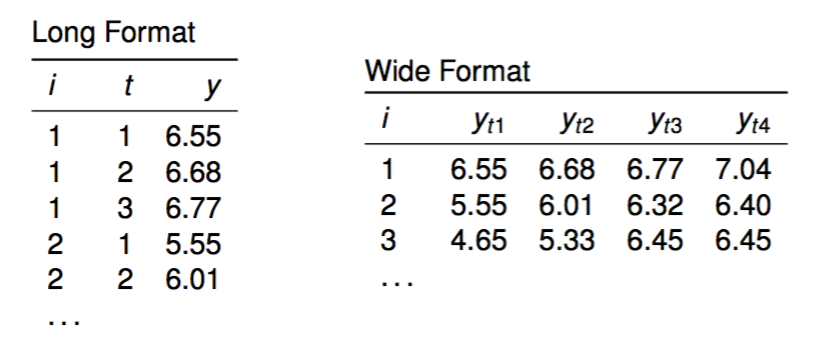
\includegraphics{figs/longwide.png}
\caption{\(i\) indiziert Einheiten, \(t\) indiziert Messzeitpunkte, \(y\) ist eine Variable}
\end{figure}

\begin{itemize}
\item
  Die Modelle in diesem Workshop nutzen das \emph{long format}
\item
  Datensätze können von einem ins andere Format transformiert werden, z.B. im \texttt{tidyverse}:

  \begin{itemize}
  \tightlist
  \item
    \texttt{tidyr::gather()} und \texttt{tidyr::spread()} (verwende ich in \texttt{R/data.R}) oder
  \item
    \texttt{tidyr::pivot\_longer()} und \texttt{tidyr::pivot\_wider()}
  \end{itemize}
\end{itemize}

\hypertarget{beispiel-daten}{%
\section{Beispiel-Daten}\label{beispiel-daten}}

\begin{itemize}
\item
  Titel: Soziale Normen im alltäglichen Umgang mit den Konsequenzen der Corona-Krise
\item
  sponsored by Jule Scheper und Sophie Bruns
\item
  Thema der Erhebung: Die Corona-Pandemie hat Regierungen auf der ganzen Welt dazu veranlasst, Reglungen zur Reduzierung der raschen Ausbreitung des Virus einzuführen. Die deutsche Bundesregierung hat am 22. März 2020 mehrere Maßnahmen zur Einschränkung sozialer Kontakte beschlossen. Diese Einschränkungen im sozialen Leben sind vollkommen neu und jede*r Einzelne muss sich auf diese Regelungen und die neue Lebenssituation einstellen. Diese Studie beschäftigt sich mit der Frage, wie Menschen sich im Alltag mit der Corona-Pandemie beschäftigen und wie sie mit den Regelungen zur Beschränkung sozialer Kontakte umgehen. Im Mittelpunkt der Untersuchung steht die Entstehung und Veränderung von sozialen Normen und persönlichen Einstellungen zur Beschränkung sozialer Kontakte über die Zeit.
\item
  Im Rahmen des Workshops steht der Einfluss der sozialen Normen und der eigenen Einstellung zum Verhalten auf das tatsächliche Social Distancing-Verhalten im Mittelpunkt.
\item
  Zeitraum der Erhebung: 1.4.-28.4.2020
\item
  Datum der Messzeitpunkte: Die Befragung besteht aus vier Wellen. Jede Welle war für eine Woche im Feld und bezog sich immer auf die vorherige Kalenderwoche.

  \begin{itemize}
  \tightlist
  \item
    Welle 1: Erhebungszeitraum vom 1.4.-7.4., Bezugszeitraum vom 23.3. bis 29.4.
  \item
    Welle 2: Erhebungszeitraum vom 8.4.-14.4., Bezugszeitraum vom 30.3. bis 5.4.
  \item
    Welle 3: Erhebungszeitraum vom 15.4.-21.4., Bezugszeitraum vom 6.4. bis 12.4.
  \item
    Welle 4: Erhebungszeitraum vom 22.4.-28.4., Bezugszeitraum vom 13.4. bis 19.4.
  \end{itemize}
\item
  Nachvollziehen der Aufbereitung in \texttt{R/data.R}
\item
  Direkt laden (z.B. für Übungen) aus \texttt{R/data/data.rds}
\item
  Der Datensatz ist bereits im \emph{long format}. \texttt{IDsosci} ist der Indikator für die Person, \texttt{wave} ist der Indikator für die Erhebungswelle.
\end{itemize}

\hypertarget{inhaltliche-variablen-im-datensatz}{%
\subsection*{Inhaltliche Variablen im Datensatz}\label{inhaltliche-variablen-im-datensatz}}
\addcontentsline{toc}{subsection}{Inhaltliche Variablen im Datensatz}

\begin{itemize}
\tightlist
\item
  Alter, Geschlecht (Dummy für weiblich), Bildung und Kollektivismus sind konstante Personenmerkmale.
\item
  Alle übrigen Variablen wurden in den vier Wellen wiederholt gemessen (mit Ausnahme von \texttt{desnorm4}, \texttt{injnorm4}, \texttt{verh4-6}, \texttt{verhint4-6}, die erst ab Welle 2 erfasst wurden).
\end{itemize}

\begin{tabular}{l|l}
\hline
Variablenname & Label\\
\hline
alter & Alter\\
\hline
besorg1 & Ich bin besorgt, wenn ich an Corona denke.\\
\hline
bildung & Bildungsabschluss\\
\hline
desnormp1 & …sind in der letzten Woche rausgegangen, auch wenn es sich nicht um einen Arztbesuch, Arbeitsweg, Spaziergang/Sport, Einkauf oder Hilfestellungen handelte.\\
\hline
desnormp2 & …haben sich in der letzten Woche in ihrer Freizeit mit mehr als einer anderen Person getroffen, die nicht im gleichen Haushalt lebt.\\
\hline
desnormp3 & …haben in der letzten Woche weniger als 1,5 Meter Abstand zu Personen gehalten, die nicht im gleichen Haushalt leben.\\
\hline
desnormp4 & ...haben sich in der letzten Woche strikt an die Maßnahmen zur Beschränkung sozialer Kontakte gehalten.\\
\hline
ein1 & Ich finde es in Ordnung, wenn man rausgeht, auch wenn es sich nicht um einen Arztbesuch, Arbeitsweg, Spaziergang/Sport, Einkauf oder Hilfe handelt.\\
\hline
ein2 & Ich finde es in Ordnung, wenn man sich in seiner Freizeit mit mehr als einer anderen Person trifft, die nicht im gleichen Haushalt lebt.\\
\hline
ein3 & Ich finde es in Ordnung, wenn man weniger als 1,5 Meter Abstand zu Personen hält, die nicht im gleichen Haushalt leben.\\
\hline
ein4 & Ich finde es wichtig, dass die Empfehlung zur Beschränkung sozialer Kontakte strikt eingehalten werden.\\
\hline
ein5 & Ich finde es richtig, dass generell Abstand gehalten werden soll.\\
\hline
injnormp1 & …finden es in Ordnung, wenn man rausgeht, auch wenn es sich nicht um einen Arztbesuch, Arbeitsweg, Spaziergang/Sport, Einkauf oder Hilfestellungen handelt.\\
\hline
injnormp2 & … finden es in Ordnung, wenn man sich in seiner Freizeit mit mehr als einer anderen Person trifft, die nicht im gleichen Haushalt lebt.\\
\hline
injnormp3 & …finden es in Ordnung, wenn man weniger als 1,5 Meter Abstand zu Personen hält, die nicht im gleichen Haushalt leben.\\
\hline
injnormp4 & ...finden es in Ordnung, wenn man sich strikt an die Maßnahmen zur Beschränkung sozialer Kontakte hält.\\
\hline
kollek & Ich würde tun, was für die Gemeinschaft am besten ist.\\
\hline
kompeer\_s1 & Freunde\\
\hline
kompeer\_s2 & Familie und Partner oder Partnerin\\
\hline
kompeer\_s3 & Bekannte (z.B. Arbeitskollegen und -kolleginnen, Vereinsmitglieder)\\
\hline
kompeer\_s4 & Prominente und/oder Influencer\\
\hline
med1 & Zeitungen \& Zeitschriften (z.B. Die ZEIT, Bild, Focus, der Spiegel)\\
\hline
med2 & Öffentlich-rechtliche Fernsehsender (z.B. ARD, ZDF, h1)\\
\hline
med3 & Private Fernsehsender (z.B. RTL, ProSieben)\\
\hline
med4 & Öffentlich-Rechtliche Radiosender (z.B. DLF, n-joy, NDR)\\
\hline
med5 & Private Radiosender (z.B. 89.0 RTL, ffn)\\
\hline
sex & Geschlecht W4 dummy\\
\hline
stress & Ich fühle mich durch die Corona-Pandemie gestresst.\\
\hline
verh1 & Ich bin rausgegangen, auch wenn es sich nicht um einen Arztbesuch, Arbeitsweg, Einkauf, Spaziergang/Sport oder Hilfestellung gehandelt hat.\\
\hline
verh2 & Ich habe mich mit mehr als einer Person getroffen, die nicht in meinem Haushalt lebt.\\
\hline
verh3 & Ich habe weniger 1,5 Meter Abstand zu Personen gehalten, die nicht in meinem Haushalt leben.\\
\hline
verh4 & Ich habe mich strikt an die Maßnahmen zur Beschränkung sozialer Kontakte gehalten.\\
\hline
verh5 & Ich habe mich im Privaten mit Freunden oder Familienmitgliedern getroffen, die nicht in meinem Haushalt leben.\\
\hline
verh6 & Ich war länger draußen als für einen üblichen Spaziergang (z.B. saß auf der Wiese oder am See).\\
\hline
verhint1 & Rausgehen, auch wenn es sich nicht um einen Arztbesuch, Arbeitsweg, Einkauf, Spaziergang/Sport oder Hilfestellung handelt.\\
\hline
verhint2 & Mich mit mehr als einer Person treffen, die nicht in meinem Haushalt lebt.\\
\hline
verhint3 & Weniger als 1,5 Meter Abstand zu Personen halten, die nicht in meinem Haushalt leben.\\
\hline
verhint4 & Mich strikt an die Maßnahmen zur Beschränkung sozialer Kontakte halten.\\
\hline
verhint5 & Mich im Privaten mit Freunden oder Familienmitgliedern treffen, die nicht in meinem Haushalt leben.\\
\hline
verhint6 & Mich länger draußen aufhalten als für einen üblichen Spaziergang (z.B. auf der Wiese oder am See sitzen).\\
\hline
veruns & Ich bin verunsichert durch die Corona-Krise.\\
\hline
\end{tabular}

\hypertarget{pooled-ols-wrong}{%
\section{Pooled OLS (WRONG!)}\label{pooled-ols-wrong}}

\begin{itemize}
\tightlist
\item
  Als erstes Beispiel wollen wir uns einer klassischen Frage aus der Theory of Planned Behavior zuwenden. Wir interessieren uns für den Effekt der Verhaltensintention auf das (berichtete) Verhalten (schließlich würden wir zum Start des Workshops ja gerne etwas finden ;)). Konkret betrachten wir den Effekt des Vorhabens, entgegen der Empfehlungen ohne relevanten Grund die Wohnung zu verlassen, auf den Selbstbericht, dies auch zu tun. Die beiden relevanten Variablen sind \texttt{verh1} und \texttt{verhint1}. Höhere Werte bedeuten eine häufigere Ausübung des Verhaltens bzw. eine höhere Wahrscheinlichkeit, das Verhalten auszuüben (gemessen auf Skala von 1 bis 5).
\item
  Die Abbildung zeigt die Entwicklung der beiden Variablen über die vier Wellen für 10 zufällig ausgewählte Personen.
\end{itemize}

\begin{Shaded}
\begin{Highlighting}[]
\NormalTok{id_smple =}\StringTok{ }\KeywordTok{sample}\NormalTok{(}\KeywordTok{unique}\NormalTok{(d}\OperatorTok{$}\NormalTok{IDsosci), }\DecValTok{10}\NormalTok{)}

\NormalTok{d }\OperatorTok\StringTok{ }\KeywordTok{filter}\NormalTok{(IDsosci }\OperatorTok\StringTok{ }\NormalTok{id_smple) }\OperatorTok\StringTok{ }\KeywordTok{select}\NormalTok{(IDsosci, wave, verh1, verhint1) }\OperatorTok\StringTok{ }
\StringTok{    }\KeywordTok{gather}\NormalTok{(variable, value, }\OperatorTok{-}\NormalTok{IDsosci, }\OperatorTok{-}\NormalTok{wave) }\OperatorTok\StringTok{ }\KeywordTok{ggplot}\NormalTok{(}\KeywordTok{aes}\NormalTok{(wave, value, }\DataTypeTok{group =}\NormalTok{ IDsosci, }
    \DataTypeTok{color =}\NormalTok{ IDsosci)) }\OperatorTok{+}\StringTok{ }\KeywordTok{geom_line}\NormalTok{(}\DataTypeTok{position =} \KeywordTok{position_jitter}\NormalTok{(}\DataTypeTok{height =} \FloatTok{0.1}\NormalTok{, }\DataTypeTok{width =} \DecValTok{0}\NormalTok{), }
    \DataTypeTok{show.legend =} \OtherTok{FALSE}\NormalTok{) }\OperatorTok{+}\StringTok{ }\KeywordTok{facet_wrap}\NormalTok{(}\StringTok{"variable"}\NormalTok{)}
\end{Highlighting}
\end{Shaded}

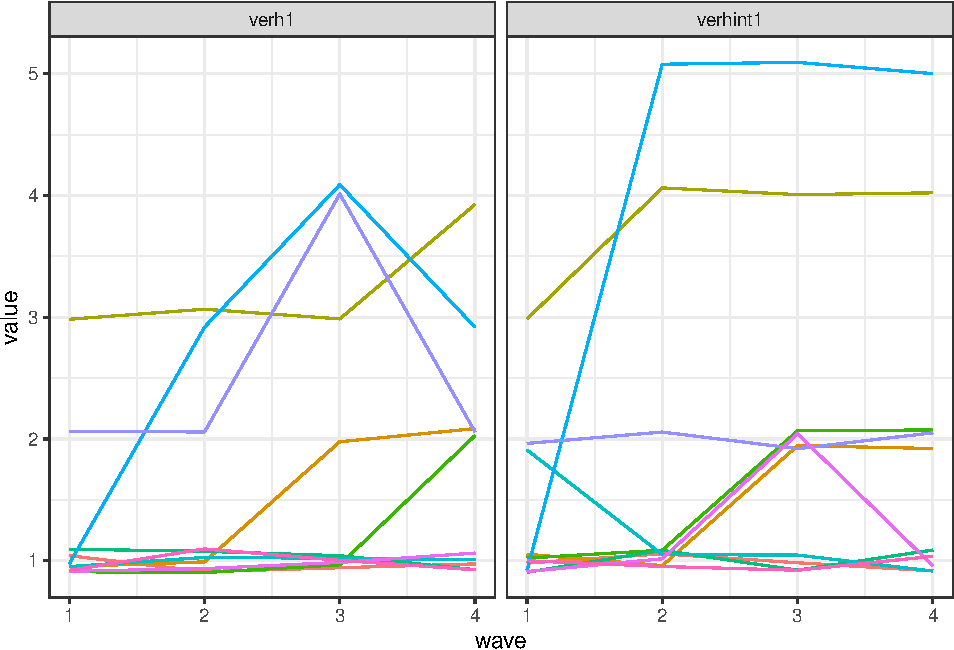
\includegraphics{workshop_panel_files/figure-latex/vis-ex1-1.pdf}

\begin{itemize}
\tightlist
\item
  Das einfachste Modell, diesen Effekt zu schätzen, ist eine einfache OLS Regression der Verhaltensintention auf das Verhalten.
\end{itemize}

\begin{Shaded}
\begin{Highlighting}[]
\KeywordTok{lm}\NormalTok{(verh1 }\OperatorTok{~}\StringTok{ }\NormalTok{verhint1, }\DataTypeTok{data =}\NormalTok{ d) }\OperatorTok\StringTok{ }\KeywordTok{tidy}\NormalTok{() }\OperatorTok\StringTok{ }\KeywordTok{mutate_if}\NormalTok{(is.numeric, round, }\DecValTok{2}\NormalTok{)}
\end{Highlighting}
\end{Shaded}

\begin{verbatim}
## # A tibble: 2 x 5
##   term        estimate std.error statistic p.value
##   <chr>          <dbl>     <dbl>     <dbl>   <dbl>
## 1 (Intercept)     0.46      0.02      19.2       0
## 2 verhint1        0.59      0.01      53.8       0
\end{verbatim}

\begin{itemize}
\tightlist
\item
  Das Modell besagt, dass die Häufigkeit, ohne triftigen Grund raus zu gehen, mit jedem Punkt auf der Intentionsskala um ca. \(b_{verhint1} = 0.6\) Punkte steigt.
\end{itemize}

\hypertarget{warum-ist-pooled-ols-immer-falsch-statistische-theorie}{%
\subsection*{Warum ist Pooled OLS immer falsch? Statistische Theorie}\label{warum-ist-pooled-ols-immer-falsch-statistische-theorie}}
\addcontentsline{toc}{subsection}{Warum ist Pooled OLS immer falsch? Statistische Theorie}

\begin{itemize}
\tightlist
\item
  Wir nennen dieses Modell \emph{pooled} OLS, da alle Beobachtungen einfach zusammengeworfen werden, ohne zu beachten, dass einige von ihnen zusammen gehören, da sie von denselben Personen stammen.
\end{itemize}

\begin{enumerate}
\def\labelenumi{\arabic{enumi})}
\tightlist
\item
  Exogenitätsannahme ist verletzt, \(E(u_i|x_i) \neq 0\)

  \begin{itemize}
  \tightlist
  \item
    Korrelationen zwischen den Variablen \(x\) gehen auf nicht gemessene Eigenschaften der Einheiten zurück, z.B. Eigenschaften der Person \(z_i\), die sowohl \(x_i\) als auch \(y_i\) beeinflussen.
  \item
    Auch bekannt als \emph{omitted variable bias}
  \item
    Könnte behoben werden, wenn alle \(z_i\) im Modell wären; diese Idee wird später wichtig
  \end{itemize}
\item
  Annahmen Homoskedastizität und unkorrelierte Residuen sind (wahrscheinlich) verletzt

  \begin{itemize}
  \tightlist
  \item
    Systematische Variation der Residuen zwischen Einheiten
  \item
    Wahrscheinlich serielle Korrelationen durch die zeitliche Abhängigkeit der Messungen
  \end{itemize}
\item
  Annahme der Unabhängigkeit der Beobachtungen verletzt

  \begin{itemize}
  \tightlist
  \item
    Überschätzung der Information von abhängigen Fällen (dieselbe Information ist mehrmals im Datensatz)

    \begin{itemize}
    \tightlist
    \item
      Zu kleine Standardfehler, zu große Zahl der Freiheitsgrade in Signifikanz-Tests
    \end{itemize}
  \item
    Die wahre Fallzahl (effective sample size) ist kleiner als Zahl der Zeilen im Datensatz (\emph{long format})
  \end{itemize}
\end{enumerate}

\hypertarget{warum-ist-pooled-ols-immer-falsch-inhaltliche-uxfcberlegungen}{%
\subsection*{Warum ist pooled OLS immer falsch? Inhaltliche Überlegungen}\label{warum-ist-pooled-ols-immer-falsch-inhaltliche-uxfcberlegungen}}
\addcontentsline{toc}{subsection}{Warum ist pooled OLS immer falsch? Inhaltliche Überlegungen}

\begin{itemize}
\tightlist
\item
  Unser Ziel ist es, den wahren kausalen Effekt von \(X\) auf \(Y\) zu schätzen.
\item
  Pooled OLS vermischt aber zwei Quellen von Unterschieden in den Daten: Den (kausalen) Effekt innerhalb der Personen (within) und die Unterschiede zwischen Personen (between).
\item
  Within und between Effekte können sich in Größe und sogar in der Richtung unterscheiden!
\item
  Die Schätzung aus einem pooled OLS Modell vermischt den kausalen Effekt und die interindividuellen Unterschiede.
\item
  In der Sprache von Interventionsstudien ist das ein Selbstselektions-Problem: Was passiert, wenn Personen, die vor dem Treatment \(x\) schon höhere Werte in \(y\) haben, das Treatment häufiger auswählen als Personen, die niedrig in \(x\) sind?
\item
  Außerdem fällt auf, dass im einfachen OLS Modell nichts darauf hindeutet, dass es sich um Paneldaten handelt. Selbst wenn wir die genannten Probleme nicht hätten, hätten wir auch nichts durch die Paneldaten gewonnen.
\end{itemize}

\hypertarget{pooled-ols-within-und-between---eine-illustration}{%
\subsection*{Pooled OLS, within und between - eine Illustration}\label{pooled-ols-within-und-between---eine-illustration}}
\addcontentsline{toc}{subsection}{Pooled OLS, within und between - eine Illustration}

\begin{itemize}
\item
  Zum Abschluss noch ein imaginäres Beispiel, um den Unterschied von intraindividuellen (within) Effekten und interindividuellen Unterschieden zu verdeutlichen. Wir führen eine Panel-Studie mit acht Personen und sechs Messzeitpunkten zum Zusammenhang von Bier-Konsum und Hangover durch. Wir interessieren uns für die kausale Frage, ob mehr Bier zu einem schlimmeren Kater führt.
\item
  In der pooled OLS Analyse wird einfach die Regressionsgerade durch alle Beobachtung gelegt. Es zeigt sich ein negativer Zusammenhang. Je mehr Bier konsumiert wurde, desto schwächer fällt der Hangover aus.
\end{itemize}

\begin{verbatim}
## `geom_smooth()` using formula 'y ~ x'
\end{verbatim}

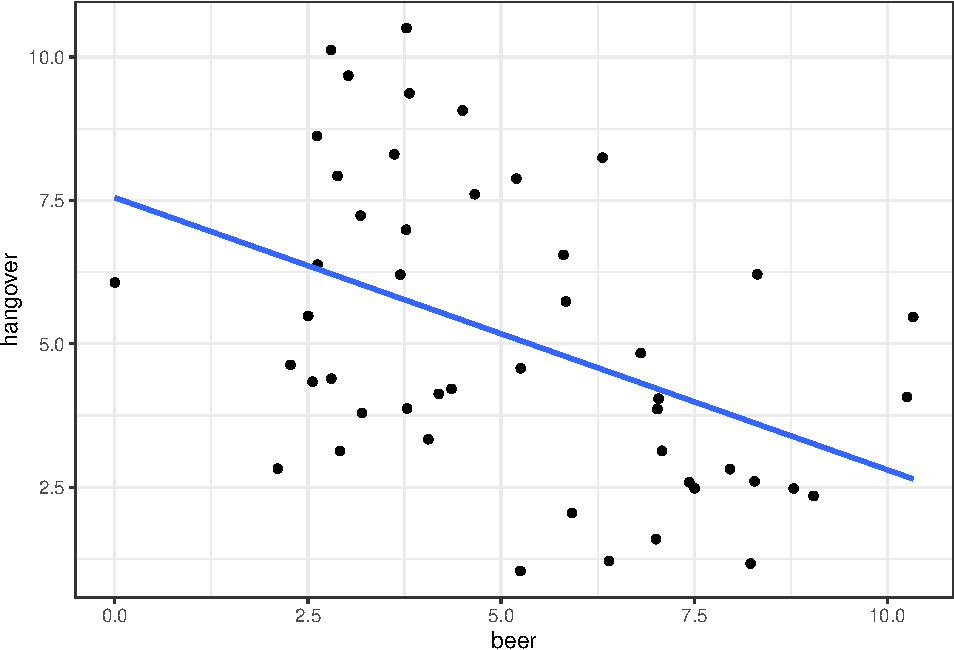
\includegraphics{workshop_panel_files/figure-latex/unnamed-chunk-8-1.pdf}

\begin{itemize}
\tightlist
\item
  Wenn wir aber für alle acht Personen separat den Zusammenhang zwischen Bierkonsum und Kater berechnen (so genanntes no pooling Modell), ergibt sich ein anderes Bild. Für alle Personen gilt mehr oder weniger deutlich: Je mehr Bier konsumiert wurde, desto stärker fällt der Hangover aus (within).
\end{itemize}

\begin{verbatim}
## `geom_smooth()` using formula 'y ~ x'
\end{verbatim}

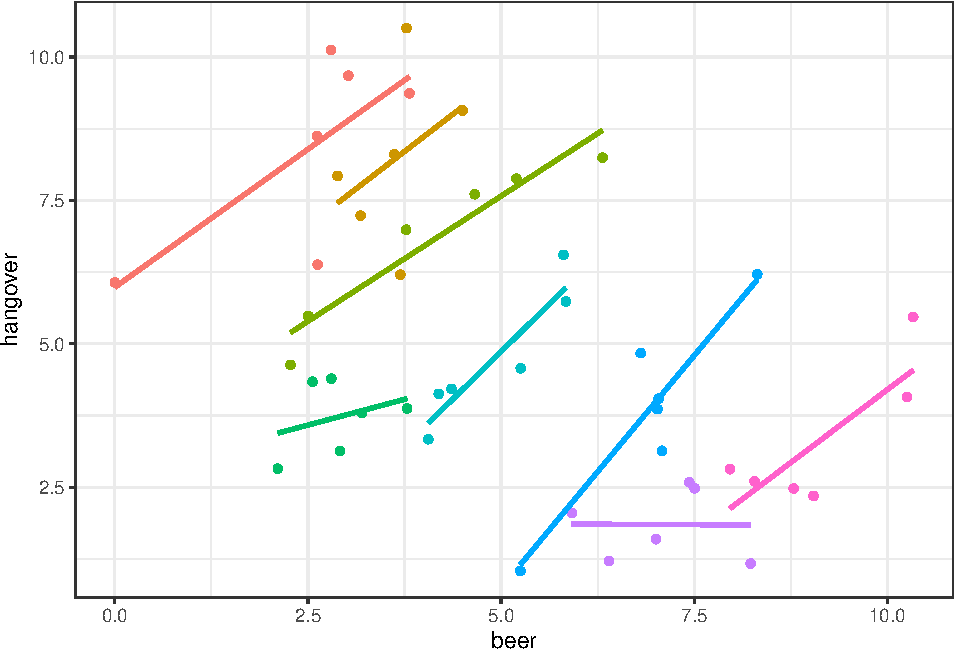
\includegraphics{workshop_panel_files/figure-latex/unnamed-chunk-9-1.pdf}

\begin{itemize}
\item
  Dazu kommt ein systematischer Unterschied zwischen den Personen (between): Personen, die im Durchschnitt mehr Bier trinken, haben im Durchschnitt einen schwächeren Hangover. Dies könnte auf eine nicht beobachte Drittvariable auf Ebene der Personen zurück gehen:

  \begin{itemize}
  \tightlist
  \item
    Vielleicht trinken Personen, die wissen, dass sie nicht so anfällig für einen Hangover sind, mehr, während Personen, die immer einen starken Kater haben, schon aus Angst vor dem nächsten Tag weniger trinken.
  \item
    Oder es ist ein Gewöhnungseffekt: Personen, die häufig viel trinken, gewöhnen sich an den Kater und nehmen ihn als weniger schlimm wahr. Oder mit Lemmy: ``A kid once said to me ``Do you get hangovers?'' I said, ``To get hangovers you have to stop drinking.''"
  \end{itemize}
\item
  Mit den vorliegenden Daten können wir die Frage nach dem Prozess nicht beantworten, da wir die Drittvariable nicht gemessen haben. Wir können aber \emph{alle} Variablen kontrollieren, die auf Personenebene liegen, z.B., indem wir wie in der Abbildung für jede Person ein separates Modell schätzen. Dann können Unterschiede zwischen den Einheiten per Modelldefinition keinen Einfluss auf die Schätzung haben. Etwas ähnliches passiert im \emph{fixed effects} Modell, das wir im nächsten Abschnitt besprechen.
\item
  An diesem Beispiel lässt sich übrigens auch schön sehen, warum uns Querschnittsdaten nicht bei der Identifikation kausaler Effekte helfen, wenn wir nicht für \(Z\) kontrollieren können. Wenn wir jede Panel-Welle für sich analysieren (die Daten also als unabhängige Querschnittserhebungen behandeln), finden wir jeweils einen negativen Zusammenhang zwischen Bierkonsum und Hangover.
\end{itemize}

\begin{verbatim}
## `geom_smooth()` using formula 'y ~ x'
\end{verbatim}

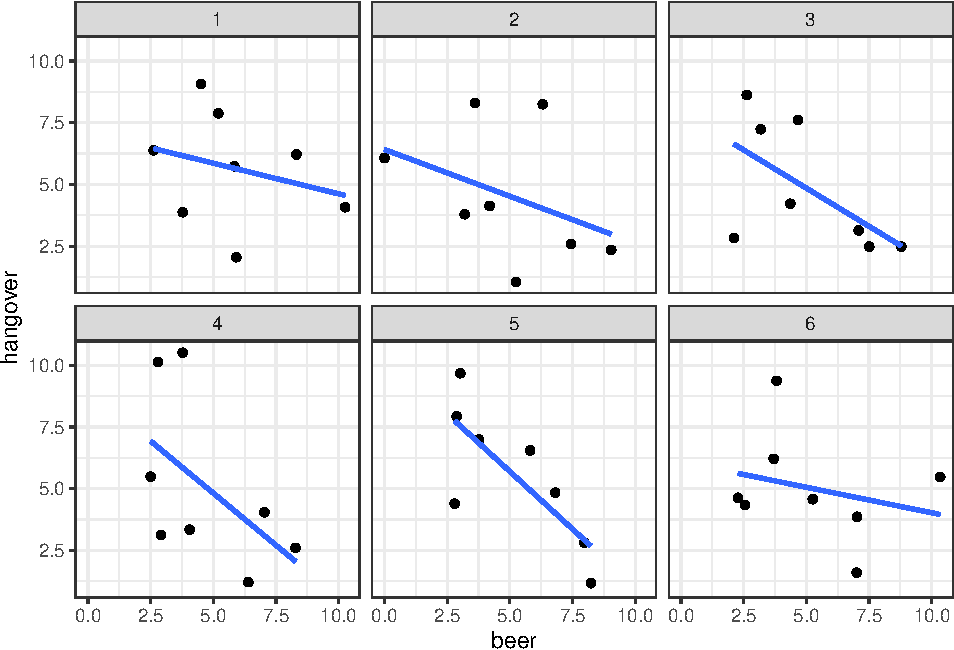
\includegraphics{workshop_panel_files/figure-latex/unnamed-chunk-10-1.pdf}

\hypertarget{fixed-effects-modelle}{%
\chapter{Fixed effects Modelle}\label{fixed-effects-modelle}}

\hypertarget{konzeptionelle-einfuxfchrung}{%
\section{Konzeptionelle Einführung}\label{konzeptionelle-einfuxfchrung}}

\begin{itemize}
\tightlist
\item
  Im ersten Teil des Abschnitts zu \emph{fixed effects} Modellen beschäftigen wir uns mit den Grundlagen der Modellierung. Dazu nutzen wir \texttt{stats::lm()} (übliche OLS-Schätzung linearer Modelle in \texttt{R}).
\end{itemize}

\hypertarget{wie-kuxf6nnen-wir-den-kausalen-within-person-effekt-mit-paneldaten-schuxe4tzen}{%
\subsection*{Wie können wir den kausalen (within-person) Effekt mit Paneldaten schätzen?}\label{wie-kuxf6nnen-wir-den-kausalen-within-person-effekt-mit-paneldaten-schuxe4tzen}}
\addcontentsline{toc}{subsection}{Wie können wir den kausalen (within-person) Effekt mit Paneldaten schätzen?}

\begin{enumerate}
\def\labelenumi{\arabic{enumi})}
\tightlist
\item
  Separate OLS Modelle für jede Person schätzen und Koeffizienten mitteln (no pooling).
\item
  Alle \(X\) und \(Y\) Variablen um die Mittelwerte der Person zentrieren (within transformation).
\item
  Dummy-Variablen für jede Person in das Regressionsmodell aufnehmen (least squares dummy variables {[}LSDV{]} estimation).
\end{enumerate}

\begin{itemize}
\tightlist
\item
  Alle drei Varianten entfernen die (beobachteten und nicht beobachten,) über die Zeit konstanten Unterschiede zwischen den Personen.
\item
  Varianten 2 und 3 entsprechen dem klassischen \emph{fixed effects} Modell. Die Unterschiede zwischen den Personen werden kontrolliert, indem die personenspezifischen Mittelwerte vor der Schätzung entfernt werden (2) oder für jede Person im Modell geschätzt werden (3).

  \begin{itemize}
  \tightlist
  \item
    \(y_{it}-\bar{y_{i}} = (x_{it} - \bar{x_{i}})'\beta + (u_{it} - \bar{u_{i}})\) oder \(y_{it} = \beta' x_{it}' + \alpha_i + u_{it}\)
  \end{itemize}
\item
  In Variante 1 dürfen die kausalen within-person Effekte zwischen den Personen variieren. Unter der Annahme homogener Treatment-Effekte (entspricht der typischen Annahme im randomisierten Between-Subject-Experiment) entspricht das Ergebnis asymptotisch den Varianten 2 und 3.

  \begin{itemize}
  \tightlist
  \item
    Der Schätzer ist aber weniger effizient, da zufällige Unterschiede in den Effekten zwischen den Personen aufgegriffen werden.
  \item
    Im letzten Teil des Abschnitts zum within-between-Modell kommen wir auf diesen Punkt zurück, wenn wir die Annahme homogener Treatment-Effekte lockern.
  \end{itemize}
\end{itemize}

\hypertarget{no-pooling}{%
\subsection*{No pooling}\label{no-pooling}}
\addcontentsline{toc}{subsection}{No pooling}

\begin{Shaded}
\begin{Highlighting}[]
\NormalTok{d }\OperatorTok\StringTok{ }\KeywordTok{group_by}\NormalTok{(IDsosci) }\OperatorTok\StringTok{ }\KeywordTok{nest}\NormalTok{() }\OperatorTok\StringTok{ }\KeywordTok{mutate}\NormalTok{(}\DataTypeTok{mdls =} \KeywordTok{map}\NormalTok{(data, }\OperatorTok{~}\KeywordTok{tidy}\NormalTok{(}\KeywordTok{lm}\NormalTok{(verh1 }\OperatorTok{~}\StringTok{ }\NormalTok{verhint1, }
    \DataTypeTok{data =}\NormalTok{ .x)))) }\OperatorTok\StringTok{ }\KeywordTok{unnest}\NormalTok{(mdls) }\OperatorTok\StringTok{ }\KeywordTok{ungroup}\NormalTok{() }\OperatorTok\StringTok{ }\KeywordTok{select}\NormalTok{(}\OperatorTok{-}\NormalTok{data) }\OperatorTok\StringTok{ }\KeywordTok{na.omit}\NormalTok{() }\OperatorTok\StringTok{ }
\StringTok{    }\KeywordTok{filter}\NormalTok{(statistic }\OperatorTok{!=}\StringTok{ }\OtherTok{Inf}\NormalTok{) }\OperatorTok\StringTok{ }\KeywordTok{filter}\NormalTok{(term }\OperatorTok{==}\StringTok{ "verhint1"}\NormalTok{) }\OperatorTok\StringTok{ }\KeywordTok{mutate_if}\NormalTok{(is.numeric, }
\NormalTok{    round, }\DecValTok{2}\NormalTok{) }\OperatorTok\StringTok{ }\NormalTok{print }\OperatorTok\StringTok{ }\KeywordTok{summarise}\NormalTok{(}\DataTypeTok{estimate =} \KeywordTok{mean}\NormalTok{(estimate), }\DataTypeTok{std.error =} \KeywordTok{sqrt}\NormalTok{(}\KeywordTok{mean}\NormalTok{(std.error}\OperatorTok{^}\DecValTok{2}\NormalTok{)))  }\CommentTok{# simple approximation}
\end{Highlighting}
\end{Shaded}

\begin{verbatim}
## # A tibble: 232 x 6
##    IDsosci term     estimate std.error statistic p.value
##    <chr>   <chr>       <dbl>     <dbl>     <dbl>   <dbl>
##  1 050IPY  verhint1     1.25      0.56  2.24e+ 0    0.15
##  2 05J4R8  verhint1     0.45      0.18  2.50e+ 0    0.13
##  3 08BDZJ  verhint1     0.33      0.53  6.30e- 1    0.59
##  4 0EO9L2  verhint1     1.67      0.67  2.50e+ 0    0.13
##  5 0F5L9Z  verhint1     0         0.71  0.          1   
##  6 0KYYAJ  verhint1     0.45      0.18  2.50e+ 0    0.13
##  7 0ONV4O  verhint1     1         0     9.01e+15    0   
##  8 0ZCKB5  verhint1    -0.35      0.5  -6.90e- 1    0.56
##  9 114OWA  verhint1     0.33      0.33  1.00e+ 0    0.42
## 10 16YGN0  verhint1     0.5       0.25  2.00e+ 0    0.18
## # ... with 222 more rows
\end{verbatim}

\begin{verbatim}
## # A tibble: 1 x 2
##   estimate std.error
##      <dbl>     <dbl>
## 1    0.502     0.521
\end{verbatim}

\begin{itemize}
\tightlist
\item
  Wir erhalten für jede Person einen Schätzer mit Standardfehler. Wir können diese mitteln, um einen Schätzer des durchschnittlichen kausalen Effekts zu erhalten.
\item
  Wir müssen die Schätzer entfernen, bei denen es wegen eines perfekten Zusammenhangs oder wegen fehlender intraindividueller Varianz keine OLS Lösung gibt.
\end{itemize}

\hypertarget{within-transformation}{%
\subsection*{Within Transformation}\label{within-transformation}}
\addcontentsline{toc}{subsection}{Within Transformation}

\begin{itemize}
\tightlist
\item
  Wir ziehen von jedem Messwert den Personenmittelwert ab. In das Modell gehen dann die um den Personenmittelwert bereinigten Variablen ein.
\end{itemize}

\begin{Shaded}
\begin{Highlighting}[]
\NormalTok{d_wi =}\StringTok{ }\NormalTok{d }\OperatorTok\StringTok{ }\KeywordTok{select}\NormalTok{(IDsosci, verh1, verhint1) }\OperatorTok\StringTok{ }\KeywordTok{group_by}\NormalTok{(IDsosci) }\OperatorTok\StringTok{ }\KeywordTok{mutate}\NormalTok{(}\DataTypeTok{verh1_wi =}\NormalTok{ verh1 }\OperatorTok{-}\StringTok{ }
\StringTok{    }\KeywordTok{mean}\NormalTok{(verh1), }\DataTypeTok{verhint1_wi =}\NormalTok{ verhint1 }\OperatorTok{-}\StringTok{ }\KeywordTok{mean}\NormalTok{(verhint1)) }\OperatorTok\StringTok{ }\KeywordTok{ungroup}\NormalTok{()}

\NormalTok{d_wi }\OperatorTok\StringTok{ }\KeywordTok{select}\NormalTok{(}\OperatorTok{-}\NormalTok{IDsosci) }\OperatorTok\StringTok{ }\NormalTok{summary}
\end{Highlighting}
\end{Shaded}

\begin{verbatim}
##      verh1        verhint1      verh1_wi      verhint1_wi   
##  Min.   :1.0   Min.   :1.0   Min.   :-3.00   Min.   :-3.00  
##  1st Qu.:1.0   1st Qu.:1.0   1st Qu.:-0.25   1st Qu.:-0.25  
##  Median :1.0   Median :1.0   Median : 0.00   Median : 0.00  
##  Mean   :1.5   Mean   :1.8   Mean   : 0.00   Mean   : 0.00  
##  3rd Qu.:2.0   3rd Qu.:2.0   3rd Qu.: 0.00   3rd Qu.: 0.00  
##  Max.   :5.0   Max.   :5.0   Max.   : 3.00   Max.   : 3.00
\end{verbatim}

\begin{Shaded}
\begin{Highlighting}[]
\NormalTok{d_wi }\OperatorTok\StringTok{ }\KeywordTok{lm}\NormalTok{(verh1_wi }\OperatorTok{~}\StringTok{ }\NormalTok{verhint1_wi, }\DataTypeTok{data =}\NormalTok{ .) }\OperatorTok\StringTok{ }\KeywordTok{tidy}\NormalTok{() }\OperatorTok\StringTok{ }\KeywordTok{mutate_if}\NormalTok{(is.numeric, }
\NormalTok{    round, }\DecValTok{2}\NormalTok{)}
\end{Highlighting}
\end{Shaded}

\begin{verbatim}
## # A tibble: 2 x 5
##   term        estimate std.error statistic p.value
##   <chr>          <dbl>     <dbl>     <dbl>   <dbl>
## 1 (Intercept)     0         0.01       0         1
## 2 verhint1_wi     0.35      0.01      24.9       0
\end{verbatim}

\begin{itemize}
\tightlist
\item
  Intuitive Interpretation: Eine Abweichung vom Personen-Durchschnitt in \(X\) um einen Punkt führt zu einer Abweichung vom Personen-Durchschnitt in \(Y\) um \(b_{X}\) Punkte.
\item
  Hier: Wenn eine Person um einen Punkt wahrscheinlicher raus gehen möchte als üblich, dann wird sie 0.34 Punkte häufiger raus gehen (beides auf 5er Skalen).
\item
  Das ist durchaus ein bedeutsamer Effekt. Aber zur Erinnerung: Der naiven pooled OLS Schätzung zufolge war der Effekt fast doppelt so groß. Es scheint also auch einen Unterschied zwischen Personen zugeben. Personen, die im Durchschnitt wahrscheinlicher raus gehen wollen, gehen im Durchschnitt auf häufiger raus.
\end{itemize}

\hypertarget{least-squares-mit-dummy-variablen-lsdv}{%
\subsection*{Least Squares mit Dummy Variablen (LSDV)}\label{least-squares-mit-dummy-variablen-lsdv}}
\addcontentsline{toc}{subsection}{Least Squares mit Dummy Variablen (LSDV)}

\begin{itemize}
\tightlist
\item
  Es wird ein Dummy-Indikator für jede \(n-1\)te Person in das Modell aufgenommen.
\end{itemize}

\begin{Shaded}
\begin{Highlighting}[]
\NormalTok{d }\OperatorTok\StringTok{ }\KeywordTok{lm}\NormalTok{(verh1 }\OperatorTok{~}\StringTok{ }\NormalTok{verhint1 }\OperatorTok{+}\StringTok{ }\KeywordTok{factor}\NormalTok{(IDsosci), }\DataTypeTok{data =}\NormalTok{ .) }\OperatorTok\StringTok{ }\KeywordTok{tidy}\NormalTok{() }\OperatorTok\StringTok{ }\KeywordTok{mutate_if}\NormalTok{(is.numeric, }
\NormalTok{    round, }\DecValTok{2}\NormalTok{) }\OperatorTok\StringTok{ }\KeywordTok{print}\NormalTok{(}\DataTypeTok{n =} \DecValTok{17}\NormalTok{)}
\end{Highlighting}
\end{Shaded}

\begin{verbatim}
## # A tibble: 577 x 5
##    term                  estimate std.error statistic p.value
##    <chr>                    <dbl>     <dbl>     <dbl>   <dbl>
##  1 (Intercept)              0.65       0.28      2.31    0.02
##  2 verhint1                 0.35       0.02     21.5     0   
##  3 factor(IDsosci)02E6C8   -0.35       0.4      -0.86    0.39
##  4 factor(IDsosci)050IPY    1.21       0.4       3.01    0   
##  5 factor(IDsosci)05J4R8    0.32       0.4       0.79    0.43
##  6 factor(IDsosci)08BDZJ    0.96       0.4       2.39    0.02
##  7 factor(IDsosci)0BHGLF    0.570      0.4       1.42    0.16
##  8 factor(IDsosci)0EB6C1    0          0.4       0       1   
##  9 factor(IDsosci)0EO9L2    1.95       0.4       4.82    0   
## 10 factor(IDsosci)0F5L9Z    1.64       0.4       4.06    0   
## 11 factor(IDsosci)0KAKHF    2.2        0.4       5.44    0   
## 12 factor(IDsosci)0KYYAJ   -0.01       0.4      -0.02    0.98
## 13 factor(IDsosci)0ONV4O    0.33       0.4       0.82    0.41
## 14 factor(IDsosci)0PKFWT   -0.09       0.4      -0.22    0.83
## 15 factor(IDsosci)0ZCKB5    0.32       0.4       0.79    0.43
## 16 factor(IDsosci)114OWA    0.33       0.4       0.82    0.41
## 17 factor(IDsosci)11KVRK   -0.17       0.4      -0.43    0.67
## # ... with 560 more rows
\end{verbatim}

\begin{itemize}
\tightlist
\item
  Der Punktschätzer \(b_{X}\) entspricht genau dem Punktschätzer nach der within-person Transformation.
\item
  Zusätzlich gibt die Regressionskonstante den Mittelwert für Person 1 an und die \(n - 1\) Koeffizienten der Dummy-Variablen die Abweichung der übrigen Personen von diesem Mittelwert. Es gelten die üblichen Regeln für die Interpretation solcher Koeffizienten.
\end{itemize}

\hypertarget{welche-modellspezifikation-soll-ich-nutzen}{%
\subsection*{Welche Modellspezifikation soll ich nutzen?}\label{welche-modellspezifikation-soll-ich-nutzen}}
\addcontentsline{toc}{subsection}{Welche Modellspezifikation soll ich nutzen?}

\begin{enumerate}
\def\labelenumi{\arabic{enumi})}
\item
  Der Schätzer des durchschnittlichen kausalen Effekts in der no pooling Spezifikation ist im Vergleich zu den beiden anderen Varianten weniger effizient. Außerdem ist er praktisch schwieriger zu ermitteln, da er erst aus den Schätzern der Einzel-Modelle berechnet werden muss. Wenn wir die Annahme eines homogenen kausalen Effekts treffen (und das tun wir üblicherweise), dann gibt es keinen Grund, das no pooling Modell in der Praxis zu verwenden.
\item
  Die Spezifikationen mit within-person Transformation und LSDV ergeben dieselben Punktschätzer für den kausalen Effekt und sind insofern austauschbar.
\item
  Die Standardfehler des Modells mit einer naiven within-person Transformation (wie oben dargestellt) sind zu klein, da wir die Stichprobenmittelwerte und nicht die (mit Unsicherheit behafteten) Schätzer der Populationsmittelwerte zur Zentrierung verwenden. Die Standardfehler müssen daher angepasst werden (passiert in spezialisierten Software-Paketen automatisch).
\item
  Die LSDV Spezifikation ist in fast jedem Softwarepaket einfach umzusetzen. Mit großen Datensätzen wird aber die Schätzung langsam und der Output unübersichtlich.
\end{enumerate}

\begin{itemize}
\item
  Unabhängig von der Spezifikation gelten weiterhin alle Annahmen der (OLS) Regression. Besonders gern vergessen wird der \emph{omitted variable bias} durch nicht gemessene, über die Zeit variierende \(Z\). \emph{Fixed effects} Modelle kontrollieren nur die \(Z\), die auf konstante Merkmale der als \emph{fixed effects} spezifizierten Einheiten zurückgehen.
\item
  Insgesamt sind viele quantitative Sozialforscher*innen (v.a. die mit einer Ökonometrie-Ausbildung) der Ansicht, dass \emph{fixed effects} Modelle die beste Methode sind, um kausale Effekte aus nicht-experimentellen Daten zu schätzen.
\end{itemize}

\hypertarget{mehre-fixed-effects-in-einem-modell-perioden-effekte}{%
\subsection*{Mehre fixed effects in einem Modell -- Perioden-Effekte}\label{mehre-fixed-effects-in-einem-modell-perioden-effekte}}
\addcontentsline{toc}{subsection}{Mehre fixed effects in einem Modell -- Perioden-Effekte}

\begin{itemize}
\tightlist
\item
  Grundsätzlich können in einem Modell beliebig viele \emph{fixed effects} spezifiziert werden.
\item
  In Paneldaten ist der Erhebungszeitpunkt bzw. die Erhebungsperiode (Panelwelle) eine typische Variable, über die verschiedene, für alle Personen konstante Effekte kontrolliert werden können.
\item
  Einige Lehrbücher empfehlen, dies \emph{immer} zu tun, da kausale Effekte von Ereignissen, die für alle Einheiten konstant sind, statistisch nicht identifiziert sind.
\item
  Eine typische Spezifikation ist die Aufnahme eines \emph{fixed effects} für den Indikator der Panelwelle.
\item
  In der LSDV-Spezifikation kann einfach ein weiterer Dummy-Faktor hinzugefügt werden. Die within-person Transformation ist mathematisch komplizierter, wird aber in spezialisierten Software-Pakten im Hintergrund erledigt. Es können auch beide Spezifikationen kombiniert werden, wenn z.B. die Periodeneffekte von inhaltlichem Interesse sind und im Output angezeigt werden sollen (siehe nächsten Teilabschnitt).
\end{itemize}

\hypertarget{ein-beispiel-mit-fixed-effects-fuxfcr-personen-und-perioden}{%
\subsection*{\texorpdfstring{Ein Beispiel mit \emph{fixed effects} für Personen und Perioden}{Ein Beispiel mit fixed effects für Personen und Perioden}}\label{ein-beispiel-mit-fixed-effects-fuxfcr-personen-und-perioden}}
\addcontentsline{toc}{subsection}{Ein Beispiel mit \emph{fixed effects} für Personen und Perioden}

\begin{Shaded}
\begin{Highlighting}[]
\NormalTok{d }\OperatorTok\StringTok{ }\KeywordTok{lm}\NormalTok{(verh1 }\OperatorTok{~}\StringTok{ }\NormalTok{verhint1 }\OperatorTok{+}\StringTok{ }\KeywordTok{factor}\NormalTok{(wave) }\OperatorTok{+}\StringTok{ }\KeywordTok{factor}\NormalTok{(IDsosci), }\DataTypeTok{data =}\NormalTok{ .) }\OperatorTok\StringTok{ }\KeywordTok{tidy}\NormalTok{() }\OperatorTok\StringTok{ }
\StringTok{    }\KeywordTok{mutate_if}\NormalTok{(is.numeric, round, }\DecValTok{2}\NormalTok{) }\OperatorTok\StringTok{ }\KeywordTok{print}\NormalTok{(}\DataTypeTok{n =} \DecValTok{17}\NormalTok{)}
\end{Highlighting}
\end{Shaded}

\begin{verbatim}
## # A tibble: 580 x 5
##    term                  estimate std.error statistic p.value
##    <chr>                    <dbl>     <dbl>     <dbl>   <dbl>
##  1 (Intercept)               0.6       0.28      2.13    0.03
##  2 verhint1                  0.33      0.02     19.8     0   
##  3 factor(wave)2             0.02      0.03      0.6     0.55
##  4 factor(wave)3             0.14      0.03      4.15    0   
##  5 factor(wave)4             0.12      0.03      3.41    0   
##  6 factor(IDsosci)02E6C8    -0.33      0.4      -0.83    0.41
##  7 factor(IDsosci)050IPY     1.26      0.4       3.15    0   
##  8 factor(IDsosci)05J4R8     0.34      0.4       0.85    0.39
##  9 factor(IDsosci)08BDZJ     1.01      0.4       2.53    0.01
## 10 factor(IDsosci)0BHGLF     0.59      0.4       1.48    0.14
## 11 factor(IDsosci)0EB6C1     0         0.4       0       1   
## 12 factor(IDsosci)0EO9L2     2.02      0.4       5.01    0   
## 13 factor(IDsosci)0F5L9Z     1.68      0.4       4.2     0   
## 14 factor(IDsosci)0KAKHF     2.27      0.4       5.63    0   
## 15 factor(IDsosci)0KYYAJ     0         0.4       0.01    0.99
## 16 factor(IDsosci)0ONV4O     0.34      0.4       0.84    0.4 
## 17 factor(IDsosci)0PKFWT    -0.08      0.4      -0.21    0.84
## # ... with 563 more rows
\end{verbatim}

\begin{itemize}
\tightlist
\item
  \(b_{verhint1}\) quantifiziert weiterhin den kausalen Effekt von Interesse. Er ist robust gegen die Kontrolle des Periodeneffekts.
\item
  Die \(b_{wave_t}\) zeigen den Kontrast zur ersten Welle. In diesem Fall sind liegen in der dritten und vierten Welle die Häufigkeiten des Rausgehens höher als noch in den ersten beiden Wellen.
\item
  Die \(b_{id_i}\) zeigen weiterhin den Kontrast zu Person 1 (substantiell nicht sonderlich interessant).
\end{itemize}

\hypertarget{uxfcbungsaufgaben-1}{%
\section{Übungsaufgaben 1}\label{uxfcbungsaufgaben-1}}

\begin{enumerate}
\def\labelenumi{\arabic{enumi})}
\tightlist
\item
  Schätze den kausalen Effekt der Einstellung zum Verhalten, weniger als 1.5m Abstand zu Personen zu halten, die nicht im gleichen Haushalt leben \texttt{ein3}, auf die diesbezügliche Verhaltensintention (\texttt{verhint3}).

  \begin{itemize}
  \tightlist
  \item
    Schätze zuerst das \emph{falsche} pooled OLS Modell.
  \item
    Schätze dann das einfache \emph{fixed effects} Modell mit einer Spezifikation deiner Wahl.
  \item
    Vergleiche schließlich die Modelle mit und ohne Periodeneffekt.
  \end{itemize}
\item
  Spezifiziere, schätze und interpretiere ein eigenes bivariates \emph{fixed effects} Modell mit Daten aus dem Beispieldatensatz.
\end{enumerate}

\hypertarget{fixed-effects-modelle-in-der-praktischen-anwendung}{%
\section{\texorpdfstring{\emph{Fixed effects} Modelle in der praktischen Anwendung}{Fixed effects Modelle in der praktischen Anwendung}}\label{fixed-effects-modelle-in-der-praktischen-anwendung}}

\begin{itemize}
\tightlist
\item
  Auch wenn wir das \emph{fixed effects} Modell nur mit \texttt{stats::lm()} und der LSDV-Spezifikation schätzen können, ist die weitere Arbeit mit diesen Modellen nicht ideal - besonders, wenn wir tiefer in Detail-Anpassungen einsteigen.
\item
  Zudem wird das Schätzen mit \texttt{stats::lm()} und LSDV bei großen Datensätzen und mit vielen \emph{fixed effects} langsam.
\item
  \texttt{plm} \citep{R-plm} ist das etablierte Paket für das Schätzen von ökonometrischen Panel-Modellen in \texttt{R}. Es bietet ein einfaches Interface zu allen Standardmodellen (und zu den übrigen Klassikern der Ökonometrie, instrumental variables, differences in differences).
\item
  Das Schätzen der Modelle basiert auf OLS mit Datentransformationen im Hintergrund. Dadurch ist das Schätzen wesentlich schneller als mit einer LSDV-Spezifikation. Die notwendigen Anpassungen der Standardfehler werden ebenfalls vorgenommen.
\end{itemize}

\hypertarget{spezifikation-eines-einfachen-fixed-effects-modells-mit-plm}{%
\subsection*{\texorpdfstring{Spezifikation eines einfachen \emph{fixed effects} Modells mit \texttt{plm}}{Spezifikation eines einfachen fixed effects Modells mit plm}}\label{spezifikation-eines-einfachen-fixed-effects-modells-mit-plm}}
\addcontentsline{toc}{subsection}{Spezifikation eines einfachen \emph{fixed effects} Modells mit \texttt{plm}}

\begin{itemize}
\tightlist
\item
  Das \emph{fixed effects} Modell wird über \texttt{model\ =\ "within"} angefordert. Mit \texttt{index\ =\ "IDsosci"} wird der Indikator für die Einheiten angegeben.
\end{itemize}

\begin{Shaded}
\begin{Highlighting}[]
\NormalTok{d }\OperatorTok\StringTok{ }\KeywordTok{plm}\NormalTok{(verh1 }\OperatorTok{~}\StringTok{ }\NormalTok{verhint1, }\DataTypeTok{data =}\NormalTok{ ., }\DataTypeTok{index =} \StringTok{"IDsosci"}\NormalTok{, }\DataTypeTok{model =} \StringTok{"within"}\NormalTok{) }\OperatorTok\StringTok{ }\KeywordTok{summary}\NormalTok{()}
\end{Highlighting}
\end{Shaded}

\begin{verbatim}
## Oneway (individual) effect Within Model
## 
## Call:
## plm(formula = verh1 ~ verhint1, data = ., model = "within", index = "IDsosci")
## 
## Balanced Panel: n = 576, T = 4, N = 2304
## 
## Residuals:
##    Min. 1st Qu.  Median 3rd Qu.    Max. 
## -3.0000 -0.1635  0.0000  0.0959  3.0000 
## 
## Coefficients:
##          Estimate Std. Error t-value Pr(>|t|)    
## verhint1   0.3459     0.0161    21.5   <2e-16 ***
## ---
## Signif. codes:  0 '***' 0.001 '**' 0.01 '*' 0.05 '.' 0.1 ' ' 1
## 
## Total Sum of Squares:    702
## Residual Sum of Squares: 554
## R-Squared:      0.212
## Adj. R-Squared: -0.0512
## F-statistic: 463.924 on 1 and 1727 DF, p-value: <2e-16
\end{verbatim}

\begin{itemize}
\tightlist
\item
  Der Output von \texttt{summary()} liefert eine korrekte Beschreibung der Fallzahlen im Datensatz.
\item
  Beachte: Das angepasste \(R^2\) ist hier (wie in vielen \emph{fixed effects} Modellen) negativ. Das ist kein Grund zur Beunruhigung. Die Logik dahinter kann gut nachvollzogen werden, wenn wir uns die LSDV-Spezifikation in Erinnerung rufen. Zusätzlich zu den inhaltlich relevanten Prädiktoren enthält das Modell \(n - 1\) Prädiktoren für die Einheiten.
\end{itemize}

\hypertarget{mehre-fixed-effects-in-einem-modell-perioden-effekte-mit-plm}{%
\subsection*{\texorpdfstring{Mehre \emph{fixed effects} in einem Modell -- Perioden-Effekte mit \texttt{plm}}{Mehre fixed effects in einem Modell -- Perioden-Effekte mit plm}}\label{mehre-fixed-effects-in-einem-modell-perioden-effekte-mit-plm}}
\addcontentsline{toc}{subsection}{Mehre \emph{fixed effects} in einem Modell -- Perioden-Effekte mit \texttt{plm}}

\begin{itemize}
\tightlist
\item
  \texttt{plm} bietet zwei Möglichkeiten, die Perioden-Effekte zu spezifizieren (identische Ergebnisse, anderer Output):
\end{itemize}

\begin{enumerate}
\def\labelenumi{\arabic{enumi})}
\tightlist
\item
  Zwei Indices \texttt{index=c("IDsosci",\ "wave")} und \texttt{effect\ =\ "twoways"} für die within-Transformation.

  \begin{itemize}
  \tightlist
  \item
    Es wird ``still'' für Personen und Perioden kontrolliert, beide werden nicht im Output angezeigt.
  \item
    Das \(R^2\) bezieht sich nur auf die Varianzaufklärung durch die Prädiktoren.
  \end{itemize}
\item
  Perioden-Effekt als Dummies hinzufügen.

  \begin{itemize}
  \tightlist
  \item
    Praktisch, wenn es nur wenige Perioden gibt und wir die Ergebnisse dazu direkt im Output sehen wollen.
  \item
    Das \(R^2\) bezieht sich auf die Varianzaufklärung durch die Prädiktoren und den Perioden-Effekt.
  \end{itemize}
\end{enumerate}

\begin{Shaded}
\begin{Highlighting}[]
\NormalTok{d }\OperatorTok\StringTok{ }\KeywordTok{plm}\NormalTok{(verh1 }\OperatorTok{~}\StringTok{ }\NormalTok{verhint1, }\DataTypeTok{data =}\NormalTok{ ., }\DataTypeTok{index =} \KeywordTok{c}\NormalTok{(}\StringTok{"IDsosci"}\NormalTok{, }\StringTok{"wave"}\NormalTok{), }\DataTypeTok{model =} \StringTok{"within"}\NormalTok{, }
    \DataTypeTok{effect =} \StringTok{"twoways"}\NormalTok{) }\OperatorTok\StringTok{ }\KeywordTok{summary}\NormalTok{()}
\end{Highlighting}
\end{Shaded}

\begin{verbatim}
## Twoways effects Within Model
## 
## Call:
## plm(formula = verh1 ~ verhint1, data = ., effect = "twoways", 
##     model = "within", index = c("IDsosci", "wave"))
## 
## Balanced Panel: n = 576, T = 4, N = 2304
## 
## Residuals:
##    Min. 1st Qu.  Median 3rd Qu.    Max. 
## -3.0705 -0.1806  0.0117  0.1316  3.0494 
## 
## Coefficients:
##          Estimate Std. Error t-value Pr(>|t|)    
## verhint1   0.3288     0.0166    19.8   <2e-16 ***
## ---
## Signif. codes:  0 '***' 0.001 '**' 0.01 '*' 0.05 '.' 0.1 ' ' 1
## 
## Total Sum of Squares:    670
## Residual Sum of Squares: 546
## R-Squared:      0.185
## Adj. R-Squared: -0.0886
## F-statistic: 391.609 on 1 and 1724 DF, p-value: <2e-16
\end{verbatim}

\begin{Shaded}
\begin{Highlighting}[]
\NormalTok{mdl_pfe_pdv =}\StringTok{ }\NormalTok{d }\OperatorTok\StringTok{ }\KeywordTok{plm}\NormalTok{(verh1 }\OperatorTok{~}\StringTok{ }\NormalTok{verhint1 }\OperatorTok{+}\StringTok{ }\KeywordTok{factor}\NormalTok{(wave), }\DataTypeTok{data =}\NormalTok{ ., }\DataTypeTok{index =} \StringTok{"IDsosci"}\NormalTok{, }
    \DataTypeTok{model =} \StringTok{"within"}\NormalTok{)}
\NormalTok{mdl_pfe_pdv }\OperatorTok\StringTok{ }\KeywordTok{summary}\NormalTok{()}
\end{Highlighting}
\end{Shaded}

\begin{verbatim}
## Oneway (individual) effect Within Model
## 
## Call:
## plm(formula = verh1 ~ verhint1 + factor(wave), data = ., model = "within", 
##     index = "IDsosci")
## 
## Balanced Panel: n = 576, T = 4, N = 2304
## 
## Residuals:
##    Min. 1st Qu.  Median 3rd Qu.    Max. 
## -3.0705 -0.1806  0.0117  0.1316  3.0494 
## 
## Coefficients:
##               Estimate Std. Error t-value Pr(>|t|)    
## verhint1        0.3288     0.0166   19.79  < 2e-16 ***
## factor(wave)2   0.0200     0.0336    0.60  0.55169    
## factor(wave)3   0.1400     0.0337    4.15 0.000034 ***
## factor(wave)4   0.1178     0.0345    3.41  0.00065 ***
## ---
## Signif. codes:  0 '***' 0.001 '**' 0.01 '*' 0.05 '.' 0.1 ' ' 1
## 
## Total Sum of Squares:    702
## Residual Sum of Squares: 546
## R-Squared:      0.223
## Adj. R-Squared: -0.0377
## F-statistic: 123.824 on 4 and 1724 DF, p-value: <2e-16
\end{verbatim}

\hypertarget{robuste-standardfehler}{%
\subsection*{Robuste Standardfehler}\label{robuste-standardfehler}}
\addcontentsline{toc}{subsection}{Robuste Standardfehler}

\begin{itemize}
\item
  In der ökonometrischen Diskussion ist die Wahl der korrekten (robusten) Standardfehler sehr prominent. Diese sind robust gegen Verletzung verschiedener Annahmen, z.B. durch serielle Korrelationen der Residuen oder Heteroskedastizität.
\item
  Das \texttt{lmtest} Paket \citep{R-lmtest} ist kompatibel mit Modellen aus \texttt{plm}. Es implementiert zahlreiche robuste Schätzer bzw. Korrekturen.
\item
  Hier die ``normalen'' Standardfehler und bei Heteroskedastizität robuste Standardfehler sowie die darauf basierenden Konfidenzintervalle im Vergleich.
\item
  Weiter wollen wir dieses Thema hier nicht vertiefen. Ich empfehle für die Details der Umsetzung in \texttt{plm} \citet{plm2017} und zu einer kritischen Auseinandersetzung \citet{kingHowRobustStandard2015}.
\end{itemize}

\begin{Shaded}
\begin{Highlighting}[]
\CommentTok{# Normale SE und CI}
\NormalTok{mdl_pfe_pdv }\OperatorTok\StringTok{ }\KeywordTok{coeftest}\NormalTok{() }\OperatorTok\StringTok{ }\KeywordTok{round}\NormalTok{(}\DecValTok{3}\NormalTok{)}
\end{Highlighting}
\end{Shaded}

\begin{verbatim}
## 
## t test of coefficients:
## 
##               Estimate Std. Error t value Pr(>|t|)    
## verhint1         0.329      0.017   19.79   <2e-16 ***
## factor(wave)2    0.020      0.034    0.60    0.552    
## factor(wave)3    0.140      0.034    4.15   <2e-16 ***
## factor(wave)4    0.118      0.034    3.42    0.001 ***
## ---
## Signif. codes:  0 '***' 0.001 '**' 0.01 '*' 0.05 '.' 0.1 ' ' 1
\end{verbatim}

\begin{Shaded}
\begin{Highlighting}[]
\NormalTok{mdl_pfe_pdv }\OperatorTok\StringTok{ }\KeywordTok{coefci}\NormalTok{() }\OperatorTok\StringTok{ }\KeywordTok{round}\NormalTok{(}\DecValTok{3}\NormalTok{)}
\end{Highlighting}
\end{Shaded}

\begin{verbatim}
##                2.5 % 97.5 %
## verhint1       0.296  0.361
## factor(wave)2 -0.046  0.086
## factor(wave)3  0.074  0.206
## factor(wave)4  0.050  0.185
\end{verbatim}

\begin{Shaded}
\begin{Highlighting}[]
\CommentTok{# Heteroskedasticity-robust SE and CI}
\NormalTok{mdl_pfe_pdv }\OperatorTok\StringTok{ }\KeywordTok{coeftest}\NormalTok{(}\DataTypeTok{vcov. =}\NormalTok{ vcovHC) }\OperatorTok\StringTok{ }\KeywordTok{round}\NormalTok{(}\DecValTok{3}\NormalTok{)}
\end{Highlighting}
\end{Shaded}

\begin{verbatim}
## 
## t test of coefficients:
## 
##               Estimate Std. Error t value Pr(>|t|)    
## verhint1         0.329      0.028   11.87   <2e-16 ***
## factor(wave)2    0.020      0.029    0.69     0.49    
## factor(wave)3    0.140      0.036    3.85   <2e-16 ***
## factor(wave)4    0.118      0.032    3.70   <2e-16 ***
## ---
## Signif. codes:  0 '***' 0.001 '**' 0.01 '*' 0.05 '.' 0.1 ' ' 1
\end{verbatim}

\begin{Shaded}
\begin{Highlighting}[]
\NormalTok{mdl_pfe_pdv }\OperatorTok\StringTok{ }\KeywordTok{coefci}\NormalTok{(}\DataTypeTok{vcov. =}\NormalTok{ vcovHC) }\OperatorTok\StringTok{ }\KeywordTok{round}\NormalTok{(}\DecValTok{3}\NormalTok{)}
\end{Highlighting}
\end{Shaded}

\begin{verbatim}
##                2.5 % 97.5 %
## verhint1       0.274  0.383
## factor(wave)2 -0.037  0.077
## factor(wave)3  0.069  0.211
## factor(wave)4  0.055  0.180
\end{verbatim}

\hypertarget{aufnahme-weiterer-uxfcber-die-zeit-variierender-pruxe4diktoren}{%
\subsection*{Aufnahme weiterer über die Zeit variierender Prädiktoren}\label{aufnahme-weiterer-uxfcber-die-zeit-variierender-pruxe4diktoren}}
\addcontentsline{toc}{subsection}{Aufnahme weiterer über die Zeit variierender Prädiktoren}

\begin{itemize}
\item
  Die Aufnahme weiterer Prädiktoren, die über die Zeit variieren, erfolgt prinzipiell wie im bekannten OLS Modell.
\item
  Wichtig ist, dass es bei \emph{fixed effects} Modellen explizit um das Schätzen von kausalen Effekten geht. Entsprechend bedacht sollte die Auswahl von weiteren Prädiktoren sein. Ein ``kitchen sink'' Ansatz, den man vor allem in OLS mit Querschnittsdaten sieht, ist hier nicht angebracht. Es muss (wie eigentlich immer) darauf geachtet werden, welche Koeffizienten eines Regressionsmodells kausal interpretiert werden dürfen \citep{keeleCausalInterpretationEstimated2019}. Im \emph{fixed effects} Modell müssen wir uns das ganz explizit vergegenwärtigen und in der Ergebnisdarstellung berücksichtigen, da die Modellklasse kausale Effekte impliziert.
\item
  Nach der TPB dürfen wir dieses Modell annehmen, da die drei Prädiktoren auf derselben kausalen Stufe stehen: Verhaltensintention \textasciitilde{} Einstellung + Deskriptive Norm + Injunktive Norm. Hier schätzen wir das Modell für die Verhaltensintention \emph{Rausgehen ohne triftigen Grund}.
\end{itemize}

\begin{Shaded}
\begin{Highlighting}[]
\NormalTok{d }\OperatorTok\StringTok{ }\KeywordTok{plm}\NormalTok{(verhint1 }\OperatorTok{~}\StringTok{ }\NormalTok{ein1 }\OperatorTok{+}\StringTok{ }\NormalTok{desnormp1 }\OperatorTok{+}\StringTok{ }\NormalTok{injnormp1 }\OperatorTok{+}\StringTok{ }\KeywordTok{factor}\NormalTok{(wave), }\DataTypeTok{data =}\NormalTok{ ., }\DataTypeTok{index =} \StringTok{"IDsosci"}\NormalTok{, }
    \DataTypeTok{model =} \StringTok{"within"}\NormalTok{) }\OperatorTok\StringTok{ }\KeywordTok{tidy}\NormalTok{() }\OperatorTok\StringTok{ }\KeywordTok{mutate_if}\NormalTok{(is.numeric, round, }\DecValTok{2}\NormalTok{)}
\end{Highlighting}
\end{Shaded}

\begin{verbatim}
## # A tibble: 6 x 5
##   term          estimate std.error statistic p.value
##   <chr>            <dbl>     <dbl>     <dbl>   <dbl>
## 1 ein1              0.31      0.02     12.4     0   
## 2 desnormp1         0.05      0.03      1.56    0.12
## 3 injnormp1         0.1       0.03      3.31    0   
## 4 factor(wave)2     0.21      0.05      4.69    0   
## 5 factor(wave)3     0.24      0.05      5.3     0   
## 6 factor(wave)4     0.39      0.05      8.32    0
\end{verbatim}

\begin{itemize}
\tightlist
\item
  Vor allem die Einstellung zum Verhalten und die wahrgenommenen normativen Erwartungen haben stärkere kausale Effekte auf die Verhaltensintention.
\end{itemize}

\hypertarget{aufnahme-eines-personenmerkmals-funktioniert-nicht-ohne-warnung}{%
\subsection*{Aufnahme eines Personenmerkmals (funktioniert nicht, ohne Warnung!)}\label{aufnahme-eines-personenmerkmals-funktioniert-nicht-ohne-warnung}}
\addcontentsline{toc}{subsection}{Aufnahme eines Personenmerkmals (funktioniert nicht, ohne Warnung!)}

\begin{itemize}
\tightlist
\item
  In einer typischen Regresssionanalyse würden wir uns z.B. auch dafür interessieren, ob sich das Verhalten nach dem Geschlecht unterscheidet. Wir nehmen also \texttt{C\_sex} in die Formel auf, mit der wir das Modell in \texttt{plm} spezifizieren.
\end{itemize}

\begin{Shaded}
\begin{Highlighting}[]
\NormalTok{d }\OperatorTok\StringTok{ }\KeywordTok{plm}\NormalTok{(verh1 }\OperatorTok{~}\StringTok{ }\NormalTok{verhint1 }\OperatorTok{+}\StringTok{ }\NormalTok{C_sex }\OperatorTok{+}\StringTok{ }\KeywordTok{factor}\NormalTok{(wave), }\DataTypeTok{data =}\NormalTok{ ., }\DataTypeTok{index =} \StringTok{"IDsosci"}\NormalTok{, }\DataTypeTok{model =} \StringTok{"within"}\NormalTok{) }\OperatorTok\StringTok{ }
\StringTok{    }\NormalTok{summary}
\end{Highlighting}
\end{Shaded}

\begin{verbatim}
## Oneway (individual) effect Within Model
## 
## Call:
## plm(formula = verh1 ~ verhint1 + C_sex + factor(wave), data = ., 
##     model = "within", index = "IDsosci")
## 
## Balanced Panel: n = 576, T = 4, N = 2304
## 
## Residuals:
##    Min. 1st Qu.  Median 3rd Qu.    Max. 
## -3.0705 -0.1806  0.0117  0.1316  3.0494 
## 
## Coefficients:
##               Estimate Std. Error t-value Pr(>|t|)    
## verhint1        0.3288     0.0166   19.79  < 2e-16 ***
## factor(wave)2   0.0200     0.0336    0.60  0.55169    
## factor(wave)3   0.1400     0.0337    4.15 0.000034 ***
## factor(wave)4   0.1178     0.0345    3.41  0.00065 ***
## ---
## Signif. codes:  0 '***' 0.001 '**' 0.01 '*' 0.05 '.' 0.1 ' ' 1
## 
## Total Sum of Squares:    702
## Residual Sum of Squares: 546
## R-Squared:      0.223
## Adj. R-Squared: -0.0377
## F-statistic: 123.824 on 4 and 1724 DF, p-value: <2e-16
\end{verbatim}

\begin{itemize}
\tightlist
\item
  Geschlecht wird nicht in das Modell aufgenommen. Vorsicht: Es taucht einfach nicht im Ergebnis auf, obwohl es in der Formel steht (siehe \texttt{Call} in der Summary)
\end{itemize}

\hypertarget{warum-wird-das-personenmerkmal-nicht-ins-modell-aufgenomen}{%
\subsection*{Warum wird das Personenmerkmal nicht ins Modell aufgenomen?}\label{warum-wird-das-personenmerkmal-nicht-ins-modell-aufgenomen}}
\addcontentsline{toc}{subsection}{Warum wird das Personenmerkmal nicht ins Modell aufgenomen?}

\begin{itemize}
\tightlist
\item
  Within-person Transformation entfernt die gesamte between-person Varianz aus den Daten: \(\bar{y_{i}} = 0\).
\item
  Daher können innerhalb der Personen invariante Merkmale keine Unterschiede erklären.
\end{itemize}

\begin{Shaded}
\begin{Highlighting}[]
\NormalTok{id_smple =}\StringTok{ }\KeywordTok{sample}\NormalTok{(}\KeywordTok{unique}\NormalTok{(d}\OperatorTok{$}\NormalTok{IDsosci), }\DecValTok{100}\NormalTok{)}
\NormalTok{d }\OperatorTok\StringTok{ }\KeywordTok{filter}\NormalTok{(IDsosci }\OperatorTok\StringTok{ }\NormalTok{id_smple) }\OperatorTok\StringTok{ }\KeywordTok{select}\NormalTok{(IDsosci, wave, verh1) }\OperatorTok\StringTok{ }\KeywordTok{group_by}\NormalTok{(IDsosci) }\OperatorTok\StringTok{ }
\StringTok{    }\KeywordTok{mutate}\NormalTok{(}\DataTypeTok{verh1_within =}\NormalTok{ verh1 }\OperatorTok{-}\StringTok{ }\KeywordTok{mean}\NormalTok{(verh1)) }\OperatorTok\StringTok{ }\KeywordTok{ungroup}\NormalTok{() }\OperatorTok\StringTok{ }\KeywordTok{gather}\NormalTok{(transformation, }
\NormalTok{    value, }\OperatorTok{-}\NormalTok{IDsosci, }\OperatorTok{-}\NormalTok{wave) }\OperatorTok\StringTok{ }\KeywordTok{ggplot}\NormalTok{(}\KeywordTok{aes}\NormalTok{(wave, value, }\DataTypeTok{group =}\NormalTok{ IDsosci)) }\OperatorTok{+}\StringTok{ }\KeywordTok{geom_line}\NormalTok{(}\DataTypeTok{position =} \KeywordTok{position_jitter}\NormalTok{(}\DataTypeTok{width =} \DecValTok{0}\NormalTok{, }
    \DataTypeTok{height =} \FloatTok{0.3}\NormalTok{), }\DataTypeTok{show.legend =} \OtherTok{FALSE}\NormalTok{, }\DataTypeTok{alpha =} \FloatTok{0.5}\NormalTok{) }\OperatorTok{+}\StringTok{ }\KeywordTok{facet_wrap}\NormalTok{(}\StringTok{"transformation"}\NormalTok{)}
\end{Highlighting}
\end{Shaded}

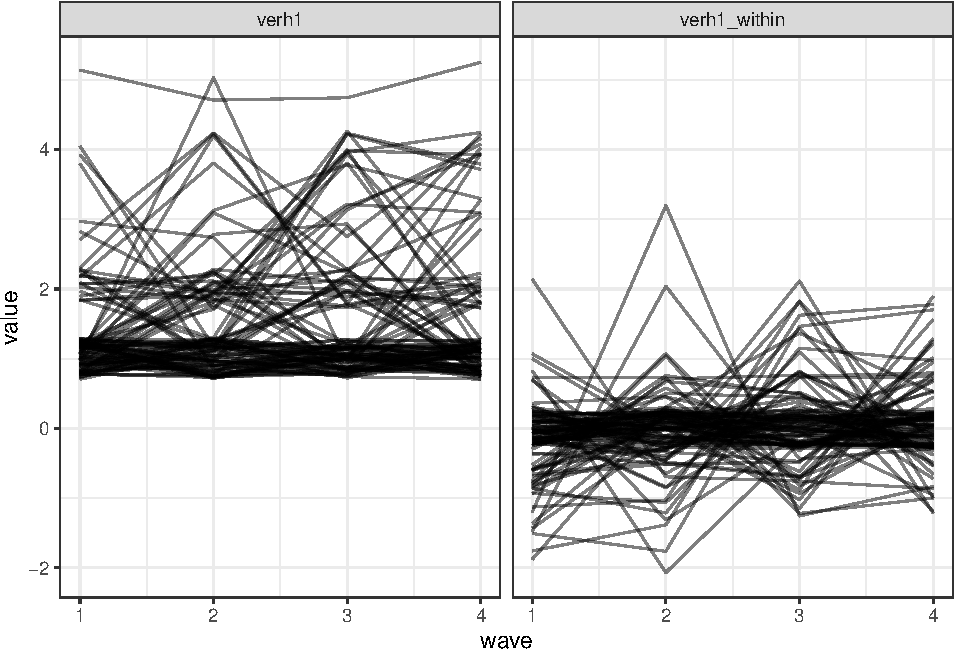
\includegraphics{workshop_panel_files/figure-latex/vis-ex2-1.pdf}

\begin{itemize}
\item
  Die Abbildung verdeutlicht dies anhand von 100 zufällig ausgewählten Personen aus dem Datensatz. Vor der Transformation gibt es (etwas) Varianz im Level des berichteten Verhaltens zwischen den Personen. Durch die Transformation verschwinden diese Unterschiede, es bleibt nur die Variation innerhalb der Personen über die Zeit.
\item
  Das gleiche gilt für Prädiktoren, die als Merkmale anderer Einheiten, die wir als \emph{fixed effects} spezifiziert haben, konstant sind. In diesem Beispiel wären dies Eigenschaften der Perioden, also z.B. neue Schutzmaßnahmen bzw. deren Lockerung, soweit sie alle Personen gleichermaßen im gleichen Zeitraum betreffen.
\end{itemize}

\hypertarget{interaktionen-mit-personenmerkmalen}{%
\subsection*{Interaktionen mit Personenmerkmalen}\label{interaktionen-mit-personenmerkmalen}}
\addcontentsline{toc}{subsection}{Interaktionen mit Personenmerkmalen}

\begin{itemize}
\tightlist
\item
  Wir können jedoch Interaktionen zwischen über die Zeit variierenden Prädiktoren und Personenmerkmalen (oder Merkmalen anderer \emph{fixed effects} Einheiten) ins Modell aufnehmen.
\item
  Bei kategoriellen Moderator-Variablen erhalten wir Schätzer der Unterschiede zwischen gruppenspezifischen Effekten, z.B. den Unterschied zwischen den Effekten der Verhaltensintention auf das Verhalten für Frauen und Männer.
\item
  Bei kontinuierlichen Moderator-Variablen gelten die üblichen Fallstricke: Der Koeffizient des Prädiktors ist nun der einfache Effekt für den Fall, dass der Moderator gleich 0 ist. Der Koeffizient des Interaktionsterms quantifiziert den Unterschied des Effekts zwischen zwei Personen, die sich auf dem Moderator um eine Einheit unterscheiden.
\end{itemize}

\begin{Shaded}
\begin{Highlighting}[]
\NormalTok{d }\OperatorTok\StringTok{ }\KeywordTok{plm}\NormalTok{(verh1 }\OperatorTok{~}\StringTok{ }\NormalTok{verhint1 }\OperatorTok{*}\StringTok{ }\NormalTok{C_sex }\OperatorTok{+}\StringTok{ }\KeywordTok{factor}\NormalTok{(wave), }\DataTypeTok{data =}\NormalTok{ ., }\DataTypeTok{index =} \StringTok{"IDsosci"}\NormalTok{, }\DataTypeTok{model =} \StringTok{"within"}\NormalTok{) }\OperatorTok\StringTok{ }
\StringTok{    }\KeywordTok{tidy}\NormalTok{() }\OperatorTok\StringTok{ }\KeywordTok{mutate_if}\NormalTok{(is.numeric, round, }\DecValTok{2}\NormalTok{)}
\end{Highlighting}
\end{Shaded}

\begin{verbatim}
## # A tibble: 5 x 5
##   term           estimate std.error statistic p.value
##   <chr>             <dbl>     <dbl>     <dbl>   <dbl>
## 1 verhint1           0.34      0.03     13.2     0   
## 2 factor(wave)2      0.02      0.03      0.59    0.55
## 3 factor(wave)3      0.14      0.03      4.14    0   
## 4 factor(wave)4      0.12      0.03      3.42    0   
## 5 verhint1:C_sex    -0.01      0.03     -0.39    0.7
\end{verbatim}

\begin{itemize}
\tightlist
\item
  Der Effekt ist in der Stichprobe für Frauen minimal schwächer als für Männer. Der Unterschied ist jedoch weder substantiell noch statistisch bedeutsam.
\end{itemize}

\hypertarget{zusammenfassung-vor--und-nachteile-des-fixed-effects-modells}{%
\section{\texorpdfstring{Zusammenfassung: Vor- und Nachteile des \emph{fixed effects} Modells}{Zusammenfassung: Vor- und Nachteile des fixed effects Modells}}\label{zusammenfassung-vor--und-nachteile-des-fixed-effects-modells}}

\begin{quote}
In many applications the whole point of using panel data is to allow for \(a_i\) to be arbitrarily correlated with the \(x_{it}\). A fixed effects analysis achieves this purpose explicitly. --- \citet{wooldridge10}, S. 300
\end{quote}

\begin{quote}
By controlling out context, FE models effectively cut out much of what is going on --- goings-on that are usually of interest to the researcher, the reader and the policy maker. We contend that models that control out, rather than explicitly model, context and heterogeneity offer overly simplistic and impoverished results that can lead to misleading interpretations. --- \citet{bellExplainingFixedEffects2015}, S. 134
\end{quote}

\begin{itemize}
\item
  Das \emph{fixed effects} Modell ist nützlich, wenn wir einen kausalen Effekt, der sich innerhalb von Einheiten (Personen) abspielt, schätzen wollen.
\item
  Das \emph{fixed effects} Modell kann keine Merkmale der Einheiten (Personen) als Prädiktoren berücksichtigen, da die gesamten einheiten(personen)spezifischen Unterschiede bereits durch die \emph{fixed effects} erklärt werden.
\item
  Wir interessieren uns aber häufig (auch) für die Unterschiede zwischen Einheiten (Personen). Das \emph{fixed effects} Modell macht Antworten auf solche Fragen unmöglich.
\item
  Ein weiterer, damit unverbundener Nachteil des \emph{fixed effects} Modells ist die starke Anfälligkeit für Messfehler. Die Transformation verringert die wahre Varianz deutlich, während große Teile der Messfehlervarianz erhalten bleiben (sie sind nicht personenspezifisch).
\end{itemize}

\hypertarget{uxfcbungsaufgaben-2}{%
\section{Übungsaufgaben 2}\label{uxfcbungsaufgaben-2}}

\begin{enumerate}
\def\labelenumi{\arabic{enumi})}
\tightlist
\item
  Schätze den kausalen Effekt der Einstellung zum Verhalten, weniger als 1.5m Abstand zu Personen zu halten, die nicht im gleichen Haushalt leben \texttt{ein3}, auf die diesbezügliche Verhaltensintention (\texttt{verhint3}). Berücksichtige dabei die Periodeneffekte der Panelwellen. Siehe dazu auch Übung 1.

  \begin{itemize}
  \tightlist
  \item
    Verwende jetzt \texttt{plm} für die Schätzung.
  \item
    Nimm zusätzlich die wahrgenommene deskriptive Norm \texttt{desnormp3} in das Modell auf.
  \item
    Prüfe, ob sich die Effekte nach Geschlecht (\texttt{C\_sex}) unterscheiden.
  \end{itemize}
\item
  Spezifiziere, schätze und interpretiere ein eigenes \emph{fixed effects} Modell mit Daten aus dem Beispieldatensatz. Nutze dabei alle Techniken (unterschiedliche Spezifikation, Standardfehler, Moderation, mehrere Prädiktoren), die du ausprobieren und zu denen du ggf. Fragen stellen willst.
\end{enumerate}

\hypertarget{random-effects-modelle}{%
\chapter{\texorpdfstring{\emph{Random effects} Modelle}{Random effects Modelle}}\label{random-effects-modelle}}

\begin{itemize}
\tightlist
\item
  In diesem Abschnitt beschäftigen wir uns mit \emph{random effects} Modellen. Zuerst führen wir die Modellklasse ein. Dann betrachten wir kurz, wie die Modelle in der Tradition der Ökonometrie mit \texttt{plm} spezifiziert werden können, bevor wir zur allgemeineren Umsetzung mit dem Paket für Mehrebenen- bzw. \emph{mixed effects} Modelle \texttt{lme4} kommen.
\end{itemize}

\hypertarget{einfuxfchrung-random-effects-modelle-fuxfcr-paneldaten}{%
\section{Einführung: Random effects Modelle für Paneldaten}\label{einfuxfchrung-random-effects-modelle-fuxfcr-paneldaten}}

\hypertarget{modellspezifikation}{%
\subsection*{Modellspezifikation}\label{modellspezifikation}}
\addcontentsline{toc}{subsection}{Modellspezifikation}

\begin{itemize}
\item
  Anstatt wie im \emph{fixed effects} Modell für jede Einheit (Person) eine separate Konstante \(\alpha_i\) zu schätzen, können wir einen ``soft constraint'' \citep[S. 257]{gelmanDataAnalysisUsing2006} setzen, dass die personenspezifischen Konstanten bzw. Residuen einer Verteilung folgen:

  \begin{itemize}
  \tightlist
  \item
    \(\alpha_{i} ∼ \mathcal{N}(\mu_{\alpha},\sigma^2_\alpha)\) mit \(i = 1,...,n\)
  \end{itemize}
\item
  Das \emph{random effects} Panel-Modell wird geschätzt als

  \begin{itemize}
  \tightlist
  \item
    \(y_{it}=x_{it}'\beta + z_i'\gamma + v_{it}\)
  \item
    \(v_{it} = \alpha_{i} + u_{it}\)
  \item
    mit \(y_{it}\) über Personen (\(i\)) und Zeit (\(t\)) variierendes Kriterium, \(x_{it}'\) über Personen und Zeit variierende Prädiktoren, \(\beta\) Koeffizienten der über Personen und Zeit variierenden Prädiktoren, \(z_i'\) über Personen variierende Prädiktoren, \(\gamma\) Koeffizienten der über Personen variierenden Prädiktoren, \(v_{it}\) gesamter Fehlerterm, \(\alpha_{i}\) personenspezifische Konstanten, \(u_{it}\) Residuen.
  \end{itemize}
\item
  Damit die Schätzer für \(\beta'\) unverzerrt sind, müssen zwei Annahmen erfüllt sein:

  \begin{enumerate}
  \def\labelenumi{\arabic{enumi}.}
  \tightlist
  \item
    Keine über die Zeit konstante Heterogenität, deren Ursache nicht im Modell ist
  \end{enumerate}

  \begin{itemize}
  \tightlist
  \item
    \({\displaystyle \operatorname {E} (\alpha _{i}|x_{it})=\operatorname {E} (\alpha _{i})=0}\)
  \end{itemize}

  \begin{enumerate}
  \def\labelenumi{\arabic{enumi}.}
  \setcounter{enumi}{1}
  \tightlist
  \item
    Keine über die Zeit variierende Heterogenität, deren Ursache nicht im Modell ist
  \end{enumerate}

  \begin{itemize}
  \tightlist
  \item
    \({\displaystyle \operatorname {E} (u_{it}|x_{it},\alpha _{i})=0,\quad t=1,...,T.}\)
  \end{itemize}
\end{itemize}

\hypertarget{vorteile-der-random-effects-modelle-fuxfcr-panel-daten}{%
\subsection*{\texorpdfstring{Vorteile der \emph{random effects} Modelle für Panel-Daten}{Vorteile der random effects Modelle für Panel-Daten}}\label{vorteile-der-random-effects-modelle-fuxfcr-panel-daten}}
\addcontentsline{toc}{subsection}{Vorteile der \emph{random effects} Modelle für Panel-Daten}

\begin{itemize}
\tightlist
\item
  Schätzer für über die Zeit konstante Prädiktoren und gleichzeitig Konstante für jede Person.
\item
  Schätzer von über die Zeit variierenden und über die Zeit konstanten Prädiktoren können verglichen werden.
\item
  Vorhersagen für neue Personen außerhalb der Stichprobe können unter Einbeziehung aller Informationen und unter Berücksichtigung der gesamten Unsicherheit gemacht werden.
\item
  Die Annahme homogener Treatment-Effekte kann gelockert werden.
\end{itemize}

\hypertarget{sind-die-annahmen-des-random-effects-modell-fuxfcr-paneldaten-jemals-erfuxfcllt}{%
\subsection*{\texorpdfstring{Sind die Annahmen des \emph{random effects} Modell für Paneldaten jemals erfüllt?}{Sind die Annahmen des random effects Modell für Paneldaten jemals erfüllt?}}\label{sind-die-annahmen-des-random-effects-modell-fuxfcr-paneldaten-jemals-erfuxfcllt}}
\addcontentsline{toc}{subsection}{Sind die Annahmen des \emph{random effects} Modell für Paneldaten jemals erfüllt?}

\begin{quote}
The only difference between RE and FE lies in the assumption they make about the relationship between υ and the observed predictors: RE models assume that the observed predictors in the model are not correlated with \(v\) while FE models allow them to be correlated.
\end{quote}

\begin{quote}
A moment's reflection on what \(v\) represents----all unmeasured time-constant factors about the respondent----should lead anyone to realize that the RE assumption is heroic in social research, to say the least.
\end{quote}

\begin{quote}
The idea that the characteristics we don't (or can't) measure (like personality or genetic influences) are uncorrelated with the things we usually do measure (like income or church attendance) is implausible. --- \citet{vaiseyWhatYouCan2017}, S. 47
\end{quote}

\hypertarget{hausman-test}{%
\subsection*{Hausman-Test}\label{hausman-test}}
\addcontentsline{toc}{subsection}{Hausman-Test}

\begin{itemize}
\tightlist
\item
  Der Hausman-Test prüft, ob das \emph{random effects} Modell konsistent ist.
\item
  Nach der traditionellen Sichtweise der Ökonometrie spricht das Verwerfen der \(H_0\) im Hausman-Test gegen das Schätzen eines \emph{random effects} Modells.
\item
  Da das \emph{random effects} Modell in der Lage ist, Forschungsfragen zu beantworten, an denen das \emph{fixed effects} Modell per Definition scheitert, lässt sich die Wahl des \emph{random effects} Modells auch inhaltlich begründen --- ohne einen Hausman-Test durchzuführen.
\item
  Der Hausman-Test kann mit der Funktion \texttt{plm::phtest()} durchgeführt werden.
\end{itemize}

\begin{Shaded}
\begin{Highlighting}[]
\KeywordTok{phtest}\NormalTok{(verh1 }\OperatorTok{~}\StringTok{ }\NormalTok{verhint1, }\DataTypeTok{data =}\NormalTok{ d, }\DataTypeTok{index =} \StringTok{"IDsosci"}\NormalTok{)}
\end{Highlighting}
\end{Shaded}

\begin{verbatim}
## 
##  Hausman Test
## 
## data:  verh1 ~ verhint1
## chisq = 301, df = 1, p-value <2e-16
## alternative hypothesis: one model is inconsistent
\end{verbatim}

\begin{itemize}
\tightlist
\item
  In diesem Beispiel spricht der Hausman-Test dagegen, ein \emph{random effects} Modell zu schätzen.
\end{itemize}

\hypertarget{random-effects-modelle-mit-plm}{%
\section{\texorpdfstring{Random effects Modelle mit \texttt{plm}}{Random effects Modelle mit plm}}\label{random-effects-modelle-mit-plm}}

\begin{itemize}
\tightlist
\item
  \emph{Random effects} Modelle für Paneldaten in der ökonometrischen Tradition lassen sich mit \texttt{plm} schätzen. Die Schätzung erfolgt auf Basis von Transformationen im Least-squares-Framework (ich habe keine Ahnung, wie das funktioniert). Ich selbst nutze diese Funktionalität in der Praxis nicht. Die Modellspezifikationen sind im Folgenden der Vollständigkeit halber kurz aufgeführt.
\end{itemize}

\begin{Shaded}
\begin{Highlighting}[]
\CommentTok{# Einfaches RE Modell}
\NormalTok{d }\OperatorTok\StringTok{ }\KeywordTok{plm}\NormalTok{(verh1 }\OperatorTok{~}\StringTok{ }\NormalTok{verhint1, }\DataTypeTok{data =}\NormalTok{ ., }\DataTypeTok{index =} \StringTok{"IDsosci"}\NormalTok{, }\DataTypeTok{model =} \StringTok{"random"}\NormalTok{) }\OperatorTok\StringTok{ }\KeywordTok{summary}\NormalTok{()}
\end{Highlighting}
\end{Shaded}

\begin{verbatim}
## Oneway (individual) effect Random Effect Model 
##    (Swamy-Arora's transformation)
## 
## Call:
## plm(formula = verh1 ~ verhint1, data = ., model = "random", index = "IDsosci")
## 
## Balanced Panel: n = 576, T = 4, N = 2304
## 
## Effects:
##                  var std.dev share
## idiosyncratic 0.3206  0.5663  0.81
## individual    0.0744  0.2728  0.19
## theta: 0.28
## 
## Residuals:
##    Min. 1st Qu.  Median 3rd Qu.    Max. 
## -2.4448 -0.1055 -0.0727  0.0389  3.6473 
## 
## Coefficients:
##             Estimate Std. Error z-value Pr(>|z|)    
## (Intercept)   0.5690     0.0276    20.6   <2e-16 ***
## verhint1      0.5320     0.0120    44.5   <2e-16 ***
## ---
## Signif. codes:  0 '***' 0.001 '**' 0.01 '*' 0.05 '.' 0.1 ' ' 1
## 
## Total Sum of Squares:    1530
## Residual Sum of Squares: 823
## R-Squared:      0.463
## Adj. R-Squared: 0.462
## Chisq: 1981.77 on 1 DF, p-value: <2e-16
\end{verbatim}

\begin{Shaded}
\begin{Highlighting}[]
\CommentTok{# Mit zusätzlichem Faktor Welle}
\NormalTok{d }\OperatorTok\StringTok{ }\KeywordTok{plm}\NormalTok{(verh1 }\OperatorTok{~}\StringTok{ }\NormalTok{verhint1, }\DataTypeTok{data =}\NormalTok{ ., }\DataTypeTok{index =} \KeywordTok{c}\NormalTok{(}\StringTok{"IDsosci"}\NormalTok{, }\StringTok{"wave"}\NormalTok{), }\DataTypeTok{model =} \StringTok{"random"}\NormalTok{, }
    \DataTypeTok{effect =} \StringTok{"twoways"}\NormalTok{) }\OperatorTok\StringTok{ }\KeywordTok{summary}\NormalTok{()}
\end{Highlighting}
\end{Shaded}

\begin{verbatim}
## Twoways effects Random Effect Model 
##    (Swamy-Arora's transformation)
## 
## Call:
## plm(formula = verh1 ~ verhint1, data = ., effect = "twoways", 
##     model = "random", index = c("IDsosci", "wave"))
## 
## Balanced Panel: n = 576, T = 4, N = 2304
## 
## Effects:
##                   var std.dev share
## idiosyncratic 0.31654 0.56262  0.80
## individual    0.07546 0.27470  0.19
## time          0.00263 0.05133  0.01
## theta: 0.285 (id) 0.585 (time) 0.254 (total)
## 
## Residuals:
##    Min. 1st Qu.  Median 3rd Qu.    Max. 
## -2.4799 -0.1144 -0.0697  0.0418  3.6722 
## 
## Coefficients:
##             Estimate Std. Error z-value Pr(>|z|)    
## (Intercept)   0.5724     0.0390    14.7   <2e-16 ***
## verhint1      0.5301     0.0121    43.7   <2e-16 ***
## ---
## Signif. codes:  0 '***' 0.001 '**' 0.01 '*' 0.05 '.' 0.1 ' ' 1
## 
## Total Sum of Squares:    1490
## Residual Sum of Squares: 817
## R-Squared:      0.453
## Adj. R-Squared: 0.453
## Chisq: 1906.68 on 1 DF, p-value: <2e-16
\end{verbatim}

\begin{Shaded}
\begin{Highlighting}[]
\CommentTok{# Mit FE für Welle}
\NormalTok{d }\OperatorTok\StringTok{ }\KeywordTok{plm}\NormalTok{(verh1 }\OperatorTok{~}\StringTok{ }\NormalTok{verhint1 }\OperatorTok{+}\StringTok{ }\KeywordTok{factor}\NormalTok{(wave), }\DataTypeTok{data =}\NormalTok{ ., }\DataTypeTok{index =} \StringTok{"IDsosci"}\NormalTok{, }\DataTypeTok{model =} \StringTok{"random"}\NormalTok{) }\OperatorTok\StringTok{ }
\StringTok{    }\KeywordTok{summary}\NormalTok{()}
\end{Highlighting}
\end{Shaded}

\begin{verbatim}
## Oneway (individual) effect Random Effect Model 
##    (Swamy-Arora's transformation)
## 
## Call:
## plm(formula = verh1 ~ verhint1 + factor(wave), data = ., model = "random", 
##     index = "IDsosci")
## 
## Balanced Panel: n = 576, T = 4, N = 2304
## 
## Effects:
##                  var std.dev share
## idiosyncratic 0.3165  0.5626  0.81
## individual    0.0755  0.2747  0.19
## theta: 0.285
## 
## Residuals:
##    Min. 1st Qu.  Median 3rd Qu.    Max. 
## -2.5049 -0.1345 -0.0672  0.0510  3.6936 
## 
## Coefficients:
##               Estimate Std. Error z-value Pr(>|z|)    
## (Intercept)    0.56642    0.03306   17.13   <2e-16 ***
## verhint1       0.53001    0.01219   43.49   <2e-16 ***
## factor(wave)2 -0.04533    0.03534   -1.28    0.200    
## factor(wave)3  0.06729    0.03539    1.90    0.057 .  
## factor(wave)4  0.00283    0.03580    0.08    0.937    
## ---
## Signif. codes:  0 '***' 0.001 '**' 0.01 '*' 0.05 '.' 0.1 ' ' 1
## 
## Total Sum of Squares:    1520
## Residual Sum of Squares: 817
## R-Squared:      0.463
## Adj. R-Squared: 0.462
## Chisq: 1983.94 on 4 DF, p-value: <2e-16
\end{verbatim}

\begin{Shaded}
\begin{Highlighting}[]
\CommentTok{# Mit Prädiktor auf Personenebene (funktioniert nicht in FE, siehe oben)}
\NormalTok{d }\OperatorTok\StringTok{ }\KeywordTok{plm}\NormalTok{(verh1 }\OperatorTok{~}\StringTok{ }\NormalTok{verhint1 }\OperatorTok{+}\StringTok{ }\NormalTok{C_sex, }\DataTypeTok{data =}\NormalTok{ ., }\DataTypeTok{index =} \KeywordTok{c}\NormalTok{(}\StringTok{"IDsosci"}\NormalTok{, }\StringTok{"wave"}\NormalTok{), }\DataTypeTok{model =} \StringTok{"random"}\NormalTok{, }
    \DataTypeTok{effect =} \StringTok{"twoways"}\NormalTok{) }\OperatorTok\StringTok{ }\KeywordTok{summary}\NormalTok{()}
\end{Highlighting}
\end{Shaded}

\begin{verbatim}
## Twoways effects Random Effect Model 
##    (Swamy-Arora's transformation)
## 
## Call:
## plm(formula = verh1 ~ verhint1 + C_sex, data = ., effect = "twoways", 
##     model = "random", index = c("IDsosci", "wave"))
## 
## Balanced Panel: n = 576, T = 4, N = 2304
## 
## Effects:
##                   var std.dev share
## idiosyncratic 0.31654 0.56262  0.80
## individual    0.07478 0.27347  0.19
## time          0.00263 0.05133  0.01
## theta: 0.283 (id) 0.585 (time) 0.253 (total)
## 
## Residuals:
##    Min. 1st Qu.  Median 3rd Qu.    Max. 
## -2.4432 -0.1535 -0.0481  0.0479  3.7019 
## 
## Coefficients:
##             Estimate Std. Error z-value Pr(>|z|)    
## (Intercept)   0.6420     0.0455    14.1   <2e-16 ***
## verhint1      0.5276     0.0122    43.4   <2e-16 ***
## C_sex        -0.1066     0.0356    -3.0   0.0027 ** 
## ---
## Signif. codes:  0 '***' 0.001 '**' 0.01 '*' 0.05 '.' 0.1 ' ' 1
## 
## Total Sum of Squares:    1500
## Residual Sum of Squares: 815
## R-Squared:      0.456
## Adj. R-Squared: 0.455
## Chisq: 1927.32 on 2 DF, p-value: <2e-16
\end{verbatim}

\hypertarget{kurze-einfuxfchrung-zu-mixed-effects-modellen}{%
\section{Kurze Einführung zu mixed effects Modellen}\label{kurze-einfuxfchrung-zu-mixed-effects-modellen}}

\begin{itemize}
\item
  Auch bekannt als \emph{random effects}, \emph{multilevel}/\emph{Mehrebenen-} oder \emph{hierarchical}/\emph{hierarchische} Modelle; das Begriffswirrwarr ist ein großes Problem \citep{gelmanDataAnalysisUsing2006}, das Denglisch macht es nicht besser.

  \begin{itemize}
  \tightlist
  \item
    siehe auch: \url{https://twitter.com/chelseaparlett/status/1262390299785072647}
  \end{itemize}
\item
  Wer mit diesen Modellen bereits vertraut ist, kann diesen Absatz überspringen.
\item
  Ganz allgemein gesprochen sind \emph{mixed effects} Modelle Regressionsmodelle für Beobachtungen von Einheiten, die in irgendeiner Art miteinander zu tun haben, also nicht unabhängig voneinander sind.
\item
  Typische Beispiele sind Schüler*innen in Klassen in Schulen, Patient*innen in Krankenhäusern, Wähler*innen in Wahlkreisen, \ldots{} .
\item
  Paneldaten haben immer eine hierarchische Struktur: Beobachtungen (Level 1) sind innerhalb der Personen (Level 2) gruppiert.
\item
  Die Bezeichnung \emph{mixed effects} geht darauf zurück, dass in den Modellen sowohl \emph{random effects} (Koeffizienten, die zwischen den Fällen innerhalb einer Gruppierung auf einer höheren Ebene variieren) als auch \emph{fixed effects} (Koeffizienten, die für alle Fälle gleich sind) spezifiziert werden.
\end{itemize}

\hypertarget{warum-wir-in-den-sozialwissenschaften-nicht-nur-die-traditionellen-uxf6konometrischen-modelle-verwenden}{%
\subsection*{Warum wir in den Sozialwissenschaften nicht nur die traditionellen ökonometrischen Modelle verwenden}\label{warum-wir-in-den-sozialwissenschaften-nicht-nur-die-traditionellen-uxf6konometrischen-modelle-verwenden}}
\addcontentsline{toc}{subsection}{Warum wir in den Sozialwissenschaften nicht nur die traditionellen ökonometrischen Modelle verwenden}

\begin{quote}
Econometrics deal mostly with non-experimental data. Great emphasis is put on specification procedures and misspecification testing. Model specifications tend therefore to be very simple, while great attention is put on the issues of endogeneity of the regressors, dependence structures in the errors and robustness of the estimators under deviations from normality. --- \citet{plm2008}
\end{quote}

\begin{itemize}
\item
  Historische Gründe und disziplinäre Entwicklungen: z.B. Ökonometriker bevorzugen fast immer Least Squares, andere Disziplinen Maximum Likelihood oder Bayesianische Methoden.
\item
  Viele Sozialwissenschaften haben kompliziertere Datenstrukturen als das typische ökonometrische Panel, z.B. mehr als zwei Ebenen, nicht-hierarchische Datenstrukturen, heterogene Treatment-Effekte, \ldots{} . Die flexible Modellierung solcher Strukturen gilt oft als wichtiger als die enger gefassten Schätz- und Identifikationsfragen, die Ökonometriker umtreiben.
\item
  Die Ökonometrie betrachtet Abhängigkeitsstrukturen als eine Störgröße, deren Einfluss in den Modellen beschränkt werden soll. Andere sozialwissenschaftliche Disziplinen interessieren sich (auch, gerade) für diese Strukturen und ihre Konsequenzen.
\end{itemize}

\hypertarget{vorteile-der-mixed-effects-modelle}{%
\subsection{\texorpdfstring{Vorteile der \emph{mixed effects} Modelle}{Vorteile der mixed effects Modelle}}\label{vorteile-der-mixed-effects-modelle}}

\begin{itemize}
\item
  \emph{Mixed effects} Modelle bieten einen einheitlichen Rahmen für die Modellierung von Datensätzen mit jeder Art von Abhängigkeitsstrukturen, seien sie hierarchisch, längsschnittlich oder eine Kombination aus beidem.
\item
  Die Schätzung basiert auf (Restricted) Maximum Likelihood, der Umstieg auf bayesianische Schätzmethoden ist relativ einfach. Im Vergleich dazu erfordern die Optionen, Tests und transformationsbasierten Least-Squares-Schätzer in der ökonometrischen Tradition erheblich mehr Einarbeitung, wenn man nicht auf eine entsprechende Ausbildung aufbauen kann.
\item
  Wer die Logik von \emph{mixed effects} Modellen einmal verstanden hat, kann die Modelle für verschiedenste Forschungsfragen und -desings einsetzen, u.a. Ländervergleiche in der komparativen Forschung, experimentelle within-subject Desings, verschiedene Längsschnittsdesigns wie experience sampling, Tagebücher, digitale Kommunikations- und Verhaltensspuren (z.B. Kommentare zu Posts auf Social Media Plattformen), \ldots{} Mehrebenenstrukturen sind überall.
\item
  Das Denken in Varianzkomponenten (siehe nächster Absatz) hilft uns, konzeptionell über die Bedeutung von Prädiktoren auf verschiedenen Ebenen nachzudenken.
\item
  Einfache praktische Umsetzung: Das Paket \texttt{lme4} ist einfach zu verwenden, wenn man bereits etwas Erfahrung mit \texttt{stats::lm()} hat, und auch ein guter Einstieg in ähnlich aufgebaute Pakte zur bayesianischen Schätzung solcher Modelle (z.B. \texttt{rstanarm}, \texttt{brms}).
\end{itemize}

\hypertarget{varianzdekomposition-und-intraklassen-korrelation}{%
\subsection*{Varianzdekomposition und Intraklassen-Korrelation}\label{varianzdekomposition-und-intraklassen-korrelation}}
\addcontentsline{toc}{subsection}{Varianzdekomposition und Intraklassen-Korrelation}

\begin{itemize}
\item
  Wir interessieren uns dafür, welcher Anteil in der Varianz in \(Y\) auf stabile Unterschiede zwischen den Personen zurück geht und welcher auf Veränderungen innerhalb von Personen (potentielle kausale Effekte).
\item
  In \emph{mixed effects} Modellen können wir die Varianz-Anteile in einem so genannten Null-Modell, das nur die Struktur der Daten abbildet, aber keine Prädiktoren enthält, bestimmen:

  \begin{itemize}
  \tightlist
  \item
    \(y_{it}= \alpha + v_{it}\) und \(v_{it} = \alpha_{i}+ u_{it}\)
  \end{itemize}
\item
  Ohne die Konstante \(\alpha\) erhalten wir

  \begin{itemize}
  \tightlist
  \item
    \(y_{it} = \alpha_{i}+ u_{it}\)
  \end{itemize}
\item
  Da die Varianzen von \(\alpha_i\) und \(u_{it}\) im Modell geschätzt werden, können wir den Anteil der personenspezifischen (Level 2) Varianz und den Anteil der idiosynkratischen Varianz in \(Y\) berechnen. Der Anteil der Level 2 Varianz an der gesamten Varianz wird auch als Intraklassen-Korrelation (intra-class correlation, ICC, \(\rho\)) bezeichnet.
\item
  In unserem Beispiel möchten wir wissen, welcher Anteil der Varianz im Verlassen der Wohnung ohne triftigen Grund auf konstante Unterschiede zwischen den Personen zurückgeht (manche Personen wollen oder müssen, aus welchen Gründen auch immer, die Wohnung häufiger verlassen als andere).
\item
  Dazu spezifizieren wir das Null-Modell mit \texttt{lme4::lmer()}. Das genaue Vorgehen beim Spezifizieren der Modelle folgt im nächsten Abschnitt. Wichtig ist an dieser Stelle, dass mit \texttt{(1\ \textbar{}\ IDsosci)} jede Person eine eigene Konstante erhält (\(\alpha_i\) in der Gleichung oben), die als Abweichung vom Gesamtmittel (\(\alpha\)) geschätzt wird.
\end{itemize}

\begin{Shaded}
\begin{Highlighting}[]
\CommentTok{# Null-Modell}
\NormalTok{m0 =}\StringTok{ }\KeywordTok{lmer}\NormalTok{(verh1 }\OperatorTok{~}\StringTok{ }\DecValTok{1} \OperatorTok{+}\StringTok{ }\NormalTok{(}\DecValTok{1} \OperatorTok{|}\StringTok{ }\NormalTok{IDsosci), }\DataTypeTok{data =}\NormalTok{ d)}

\NormalTok{m0 }\OperatorTok\StringTok{ }\KeywordTok{summary}\NormalTok{()}
\end{Highlighting}
\end{Shaded}

\begin{verbatim}
## Linear mixed model fit by REML. t-tests use Satterthwaite's method [
## lmerModLmerTest]
## Formula: verh1 ~ 1 + (1 | IDsosci)
##    Data: d
## 
## REML criterion at convergence: 5576
## 
## Scaled residuals: 
##    Min     1Q Median     3Q    Max 
## -4.139 -0.227 -0.121 -0.121  4.813 
## 
## Random effects:
##  Groups   Name        Variance Std.Dev.
##  IDsosci  (Intercept) 0.594    0.771   
##  Residual             0.407    0.638   
## Number of obs: 2304, groups:  IDsosci, 576
## 
## Fixed effects:
##             Estimate Std. Error       df t value Pr(>|t|)    
## (Intercept)   1.5286     0.0347 575.0000      44   <2e-16 ***
## ---
## Signif. codes:  0 '***' 0.001 '**' 0.01 '*' 0.05 '.' 0.1 ' ' 1
\end{verbatim}

\begin{Shaded}
\begin{Highlighting}[]
\CommentTok{# ICC 'von Hand'}
\FloatTok{0.5938}\OperatorTok{/}\NormalTok{(}\FloatTok{0.5938} \OperatorTok{+}\StringTok{ }\FloatTok{0.4065}\NormalTok{)}
\end{Highlighting}
\end{Shaded}

\begin{verbatim}
## [1] 0.59
\end{verbatim}

\begin{Shaded}
\begin{Highlighting}[]
\CommentTok{# Mit performance::icc()}
\KeywordTok{icc}\NormalTok{(m0)}
\end{Highlighting}
\end{Shaded}

\begin{verbatim}
## # Intraclass Correlation Coefficient
## 
##      Adjusted ICC: 0.594
##   Conditional ICC: 0.594
\end{verbatim}

\begin{itemize}
\item
  Die Informationen zu den Varianzkomponenten findet sich im Output von \texttt{summary()} unter \texttt{Random\ effects}. Aus diesen Angaben können wir die ICC berechnen. Oder wir nutzen die Funktion \texttt{performance::icc()}.
\item
  Fast 60\% der Varianz im Verlassen der Wohnung geht auf Unterschiede zwischen Personen zurück.
\item
  Im \emph{fixed effects} Modell wird diese Varianz einfach aus den Daten entfernt. Über mehr als die Hälfte der Unterschiede können wir mit \emph{fixed effects} Modellen also per Spezifikationslogik nichts aussagen.
\item
  Kausale Effekte innerhalb der Personen können damit \emph{maximal} für 40\% der Varianz verantwortlich sein.
\item
  Allerdings müssen wir dabei beachten, dass auch der gesamte Messfehler (zumindest die zufällige Messfehlervarianz nach der CTT) ebenfalls in diesem Varianzanteil steckt.
\item
  Wir können die Schätzer der \emph{random intercepts} für die Personen im Null-Modell auch dazu nutzen, uns einen Überblick zu verschaffen über die Verteilung der personenspezifischen Tendenz, die Wohnung ohne triftigen Grund zu verlassen. Die Schätzer können wir mit \texttt{ranef()} extrahieren, mit \texttt{broom.mixed::augment()} erhalten wir zusätzlich Standardfehler und Konfidenzintervalle in einem tidy data.frame.
\end{itemize}

\begin{Shaded}
\begin{Highlighting}[]
\CommentTok{# tibble der RE und ihre Verteilung als Histogramm}
\NormalTok{m0 }\OperatorTok\StringTok{ }\KeywordTok{ranef}\NormalTok{() }\OperatorTok\StringTok{ }\KeywordTok{augment}\NormalTok{(}\DataTypeTok{ci.level =} \FloatTok{0.95}\NormalTok{) }\OperatorTok\StringTok{ }\KeywordTok{as_tibble}\NormalTok{() }\OperatorTok\StringTok{ }\KeywordTok{print}\NormalTok{(}\DataTypeTok{n =} \DecValTok{12}\NormalTok{) }\OperatorTok\StringTok{ }
\StringTok{    }\KeywordTok{ggplot}\NormalTok{(}\KeywordTok{aes}\NormalTok{(estimate)) }\OperatorTok{+}\StringTok{ }\KeywordTok{geom_histogram}\NormalTok{()}
\end{Highlighting}
\end{Shaded}

\begin{verbatim}
## # A tibble: 576 x 8
##    grp     variable    level  estimate       qq std.error     lb    ub
##    <fct>   <fct>       <fct>     <dbl>    <dbl>     <dbl>  <dbl> <dbl>
##  1 IDsosci (Intercept) 01PQGO  -0.451  -3.13        0.295 -1.03  0.126
##  2 IDsosci (Intercept) 02E6C8  -0.451  -2.79        0.295 -1.03  0.126
##  3 IDsosci (Intercept) 050IPY   1.47    1.53        0.295  0.892 2.05 
##  4 IDsosci (Intercept) 05J4R8   0.189   0.571       0.295 -0.388 0.766
##  5 IDsosci (Intercept) 08BDZJ   1.26    1.41        0.295  0.679 1.83 
##  6 IDsosci (Intercept) 0BHGLF   0.402   0.779       0.295 -0.175 0.980
##  7 IDsosci (Intercept) 0EB6C1  -0.451  -2.62        0.295 -1.03  0.126
##  8 IDsosci (Intercept) 0EO9L2   2.32    2.02        0.295  1.75  2.90 
##  9 IDsosci (Intercept) 0F5L9Z   1.68    1.63        0.295  1.11  2.26 
## 10 IDsosci (Intercept) 0KAKHF   2.54    2.05        0.295  1.96  3.11 
## 11 IDsosci (Intercept) 0KYYAJ  -0.238  -0.00653     0.295 -0.815 0.339
## 12 IDsosci (Intercept) 0ONV4O  -0.0245  0.321       0.295 -0.602 0.553
## # ... with 564 more rows
\end{verbatim}

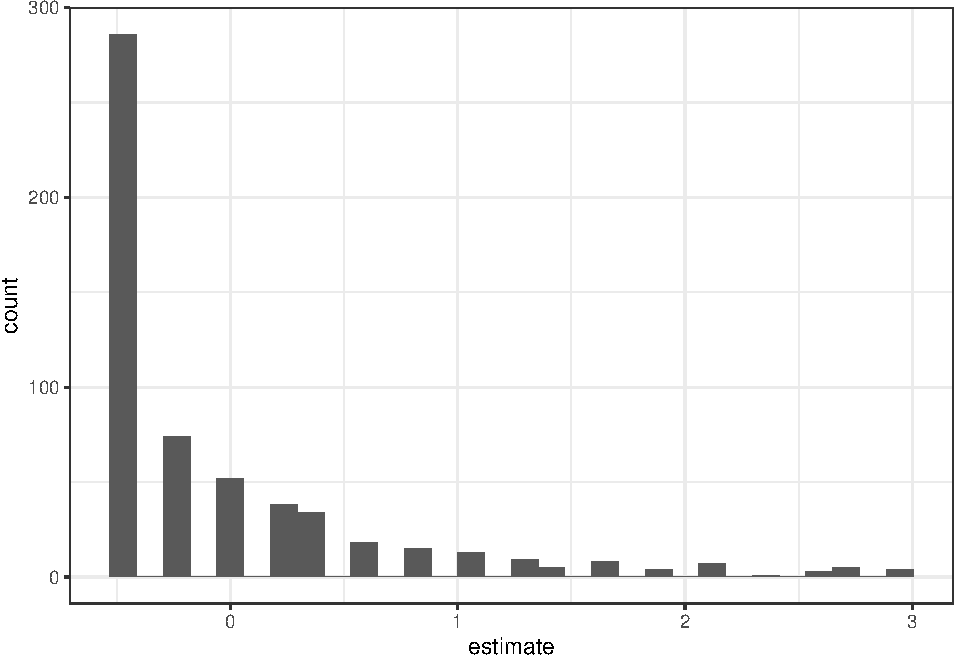
\includegraphics{workshop_panel_files/figure-latex/ranef-1.pdf}

\begin{Shaded}
\begin{Highlighting}[]
\CommentTok{# RE mit 95%-CIs (aus Darstellungsgründen nur jede fünfte Person)}
\NormalTok{m0 }\OperatorTok\StringTok{ }\KeywordTok{ranef}\NormalTok{() }\OperatorTok\StringTok{ }\KeywordTok{augment}\NormalTok{(}\DataTypeTok{ci.level =} \FloatTok{0.95}\NormalTok{) }\OperatorTok\StringTok{ }\KeywordTok{slice}\NormalTok{(}\KeywordTok{seq}\NormalTok{(}\DecValTok{1}\NormalTok{, }\KeywordTok{nrow}\NormalTok{(.), }\DataTypeTok{by =} \DecValTok{5}\NormalTok{)) }\OperatorTok\StringTok{ }
\StringTok{    }\KeywordTok{ggplot}\NormalTok{(}\KeywordTok{aes}\NormalTok{(estimate, level, }\DataTypeTok{xmin =}\NormalTok{ lb, }\DataTypeTok{xmax =}\NormalTok{ ub)) }\OperatorTok{+}\StringTok{ }\KeywordTok{geom_pointrangeh}\NormalTok{() }\OperatorTok{+}\StringTok{ }\KeywordTok{labs}\NormalTok{(}\DataTypeTok{y =} \StringTok{"IDsosci"}\NormalTok{)}
\end{Highlighting}
\end{Shaded}

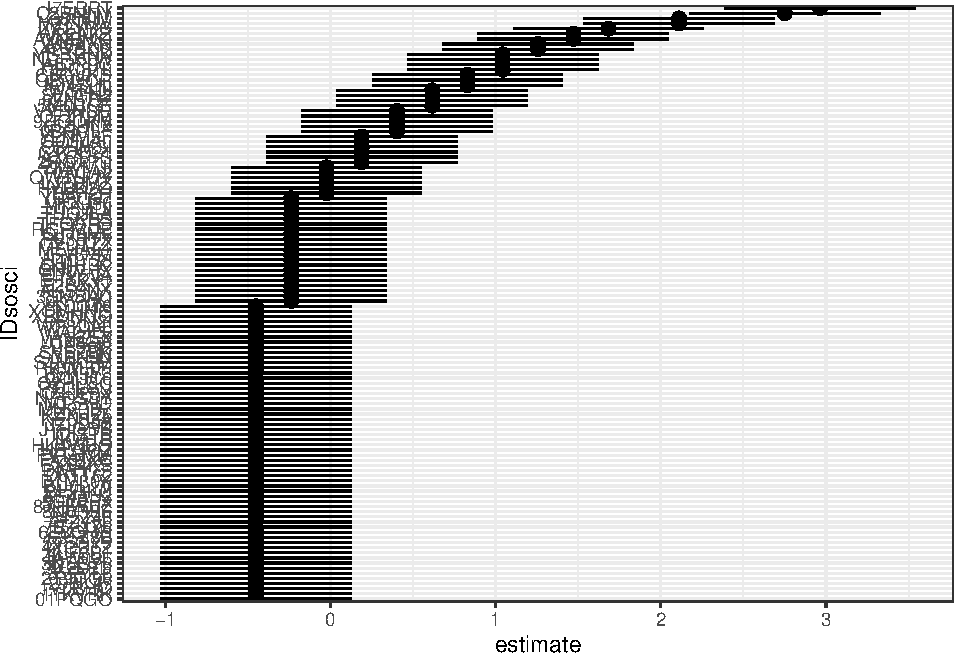
\includegraphics{workshop_panel_files/figure-latex/ranef-2.pdf}

\begin{itemize}
\tightlist
\item
  Die \emph{random intercepts} Schätzer quantifizieren die Abweichung vom Schätzer der Konstanten in der Gesamtpopulation, hier die Abweichung von 1.5. Die diskreten Werte kommen zustande, da es (wie bei einer Index-Bildung) mit 5 Ausprägungen und 4 Wellen nur eine begrenzte Anzahl an möglichen Personen-Mittelwerten gibt.
\item
  Die Mehrheit der Personen tendiert dazu, eher selten ihre Wohnung ohne triftigen Grund zu verlassen.
\end{itemize}

\hypertarget{mehr-als-ein-gruppierungsfaktor}{%
\subsection*{Mehr als ein Gruppierungsfaktor}\label{mehr-als-ein-gruppierungsfaktor}}
\addcontentsline{toc}{subsection}{Mehr als ein Gruppierungsfaktor}

\begin{itemize}
\tightlist
\item
  Mit \texttt{lme4} können prinzipiell beliebig viele und arbiträr angeordnete (sie müssen nicht hierarchisch sein) \emph{random effects} in ein Modell aufgenommen werden.
\item
  Zu viele Faktoren oder Faktoren mit zu wenigen Ausprägungen können aber zu Problemen bei der (restricted) maximum likelihood Schätzung führen (Bayesianische Schätzverfahren können hier helfen).
\item
  Wir könnten z.B. die geographische Region, in der die Personen leben, als einen weiteren, hierarchisch oberhalb der Person angesiedelten Faktor aufnehmen. Hätten wir eine sehr große Stichprobe mit ausreichend geographischer Variation, wäre dies spannend, da wir uns durchaus regionale Unterschiede vorstellen könnten.
\item
  In Panel-Modellen liegt die Idee nahe, \emph{random effects} für die Panel-Wellen aufzunehmen. Dieser Faktor ist nicht hierarchisch zu den Personen. Stattdessen gehört jede Messung zu genau einer Person und genau einer Welle. Diese Spezifikation wird auch \emph{kreuzklassifiziert} / \emph{cross-classified} / \emph{crossed} genannt.

  \begin{itemize}
  \tightlist
  \item
    Wir nehmen den Faktor Welle auf, indem wir \texttt{+\ (1\ \textbar{}\ wave)} in der Modell-Formel ergänzen.
  \item
    Da wir nur Daten aus vier Wellen haben und die Varianz zwischen den Wellen sehr klein ist, kommt die \emph{restricted maximum likelihood} Schätzung hier an ihre Grenzen. Eine Warnung wird ausgegeben. Wir könnten das Problem durch Herumfrickeln an den Einstellungen des Optimizer beheben, würden aber inhaltlich zu keiner anderen Schlussfolgerungen kommen. Um den Einstieg in die technischen Details zu vermeiden, verwenden wir hier aber das Modell mit der Warnmeldung.
  \item
    Im Weiteren lösen wir das Problem, indem wir \emph{fixed effects} für die Wellen aufnehmen.
  \end{itemize}
\end{itemize}

\begin{Shaded}
\begin{Highlighting}[]
\CommentTok{# Null-Modell mit zwei Gruppierungsfaktoren}
\KeywordTok{lmer}\NormalTok{(verh1 }\OperatorTok{~}\StringTok{ }\DecValTok{1} \OperatorTok{+}\StringTok{ }\NormalTok{(}\DecValTok{1} \OperatorTok{|}\StringTok{ }\NormalTok{IDsosci) }\OperatorTok{+}\StringTok{ }\NormalTok{(}\DecValTok{1} \OperatorTok{|}\StringTok{ }\NormalTok{wave), }\DataTypeTok{data =}\NormalTok{ d) }\OperatorTok\StringTok{ }\KeywordTok{icc}\NormalTok{(}\DataTypeTok{by_group =} \OtherTok{TRUE}\NormalTok{)}
\end{Highlighting}
\end{Shaded}

\begin{verbatim}
## Warning in checkConv(attr(opt, "derivs"), opt$par, ctrl = control$checkConv, :
## Model failed to converge with max|grad| = 0.00262857 (tol = 0.002, component 1)
\end{verbatim}

\begin{verbatim}
## # ICC by Group
## 
## Group   |   ICC
## ---------------
## IDsosci | 0.595
## wave    | 0.018
\end{verbatim}

\begin{itemize}
\tightlist
\item
  Nur ein sehr geringer Teil der gesamten Varianz geht auf über alle Personen homogene Veränderungen zwischen den Wellen zurück.
\end{itemize}

\hypertarget{uxfcbungsaufgaben-3}{%
\section{Übungsaufgaben 3}\label{uxfcbungsaufgaben-3}}

\begin{enumerate}
\def\labelenumi{\arabic{enumi})}
\tightlist
\item
  Analysiere die Varianzkomponenten in der Intention, weniger als 1.5m Abstand zu einer Person zu halten, die nicht im eigenen Haushalt lebt (\texttt{verhint3}).

  \begin{itemize}
  \tightlist
  \item
    Spezifiziere zuerst ein Modell mit \emph{random effects} für die Personen.
  \item
    Nimm dann die Welle als zweiten Gruppierungsfaktor auf.
  \end{itemize}
\item
  Analysiere die Varianzkomponenten in weiteren Variablen, die dich interessieren.
\end{enumerate}

\hypertarget{random-effects-panel-modelle-mit-lme4}{%
\section{\texorpdfstring{Random effects panel Modelle mit \texttt{lme4}}{Random effects panel Modelle mit lme4}}\label{random-effects-panel-modelle-mit-lme4}}

\hypertarget{wiederholung-der-wichtigsten-begriffe}{%
\subsection*{Wiederholung der wichtigsten Begriffe}\label{wiederholung-der-wichtigsten-begriffe}}
\addcontentsline{toc}{subsection}{Wiederholung der wichtigsten Begriffe}

\begin{itemize}
\tightlist
\item
  Ganz allgemein gesprochen ist ein \emph{mixed effects} Modell ein Modell, das \emph{fixed} und \emph{random} Koeffizienten enthält.
\item
  \citet{gelmanDataAnalysisUsing2006} verwenden die (imo) besser verständlichen Begriffe \emph{varying intercepts} (für zwischen Einheiten auf höherer Ebene variierende Regressionskonstanten) und \emph{varying slopes} (für zwischen Einheiten auf höherer Ebene variierende Regressionskoeffizienten).
\item
  Im \emph{random effects} Panelmodell sind die Einheiten auf höherer Ebene die Personen. Die Konstanten bzw. Koeffizienten variieren zwischen Personen.
\item
  In der Sprache von \emph{mixed effects} Modellen wird das einfachste Modell als \emph{fixed slope, random} (oder \emph{varying}) \emph{intercept} Modell bezeichnet.

  \begin{itemize}
  \tightlist
  \item
    Die Regressionskonstante variiert zwischen den Personen (jede Person erhält eine eigene Konstante, die aus einer Normalverteilung mit der Populationskonstante als Mittelwert und der personenspezifischen Varianz als Streuung stammt).
    Die übrigen Regressionskoeffizienten sind für alle Personen gleich (\emph{fixed}).
  \end{itemize}
\end{itemize}

\hypertarget{einfaches-random-effects-panel-modell}{%
\subsection*{Einfaches random effects panel Modell}\label{einfaches-random-effects-panel-modell}}
\addcontentsline{toc}{subsection}{Einfaches random effects panel Modell}

\begin{itemize}
\item
  Wir modellieren wieder die Häufigkeit, ohne triftigen Grund die Wohnung zu verlassen, in Abhängigkeit der Intention, dies zu tun.
\item
  Die Spezifikation in \texttt{lme4::lmer()} folgt der in \texttt{R} üblichen Logik. Das Modell enthält \texttt{verhint1} als Prädiktor mit einem für alle Personen gleichen Koeffizienten (homogener Treatment-Effekt) und \texttt{(1\ \textbar{}~IDsosci)} als \emph{varying intercept} für jede Person.
\item
  Hinweis: \texttt{lme4} selbst weist keine Freiheitsgrade und entsprechend auch keine \emph{p}-Werte für die Koeffizienten aus. Wenn -- wie hier -- zusätzlich das Paket \texttt{lmerTest} geladen wurde, werden diese automatisch ergänzt.
\end{itemize}

\begin{Shaded}
\begin{Highlighting}[]
\NormalTok{m1 =}\StringTok{ }\KeywordTok{lmer}\NormalTok{(verh1 }\OperatorTok{~}\StringTok{ }\NormalTok{verhint1 }\OperatorTok{+}\StringTok{ }\NormalTok{(}\DecValTok{1} \OperatorTok{|}\StringTok{ }\NormalTok{IDsosci), }\DataTypeTok{data =}\NormalTok{ d)}

\NormalTok{m1 }\OperatorTok\StringTok{ }\KeywordTok{summary}\NormalTok{(}\DataTypeTok{correlation =} \OtherTok{FALSE}\NormalTok{)}
\end{Highlighting}
\end{Shaded}

\begin{verbatim}
## Linear mixed model fit by REML. t-tests use Satterthwaite's method [
## lmerModLmerTest]
## Formula: verh1 ~ verhint1 + (1 | IDsosci)
##    Data: d
## 
## REML criterion at convergence: 4554
## 
## Scaled residuals: 
##    Min     1Q Median     3Q    Max 
## -4.524 -0.202 -0.085  0.165  5.793 
## 
## Random effects:
##  Groups   Name        Variance Std.Dev.
##  IDsosci  (Intercept) 0.111    0.334   
##  Residual             0.341    0.584   
## Number of obs: 2304, groups:  IDsosci, 576
## 
## Fixed effects:
##              Estimate Std. Error        df t value Pr(>|t|)    
## (Intercept)    0.5987     0.0287  975.4311    20.9   <2e-16 ***
## verhint1       0.5155     0.0122 1747.0982    42.3   <2e-16 ***
## ---
## Signif. codes:  0 '***' 0.001 '**' 0.01 '*' 0.05 '.' 0.1 ' ' 1
\end{verbatim}

\begin{itemize}
\item
  Mit jedem Punkt auf der Skala zur Verhaltensintention steigt die Häufigkeit des Rausgehens ohne triftigen Grund um 0.5 Punkte.
\item
  Wir können das Modell mit dem Prädiktor \texttt{verhint1} mit dem Null-Modell vergleichen.

  \begin{itemize}
  \tightlist
  \item
    Mit \texttt{anova()} erhalten wir verschiedene Informationskriterien und einen Likelihood Ratio (Wald) Test. Die Test-Statistik folgt einer \(\chi^2\)-Verteilung.
  \item
    Durch einen Vergleich der Varianzkomponenten der Modelle erhalten wir ein Maß, das konzeptionell ähnlich \(\Delta R^2\) interpretiert werden kann. Die Funktion \texttt{performance::r2(by\_group\ =\ TRUE)} implementiert diesen Vergleich für ein Modell und das Null-Modell. Die manuelle Berechnung ist auch schrittweise für mehre Modelle möglich, die zunehmend mehr Prädiktoren enthalten. Wichtig: Die \(\Delta R^2\)-Logik funktioniert nur in Modellen mit identischen \emph{random effects}.
  \end{itemize}
\end{itemize}

\begin{Shaded}
\begin{Highlighting}[]
\CommentTok{# Wald Test und Informationskriterien}
\KeywordTok{anova}\NormalTok{(m0, m1)}
\end{Highlighting}
\end{Shaded}

\begin{verbatim}
## Data: d
## Models:
## m0: verh1 ~ 1 + (1 | IDsosci)
## m1: verh1 ~ verhint1 + (1 | IDsosci)
##    Df  AIC  BIC logLik deviance Chisq Chi Df Pr(>Chisq)    
## m0  3 5577 5595  -2786     5571                            
## m1  4 4549 4572  -2270     4541  1031      1     <2e-16 ***
## ---
## Signif. codes:  0 '***' 0.001 '**' 0.01 '*' 0.05 '.' 0.1 ' ' 1
\end{verbatim}

\begin{Shaded}
\begin{Highlighting}[]
\CommentTok{# Reduktion der Varianz (Delta R^2) - manuell}
\DecValTok{1} \OperatorTok{-}\StringTok{ }\NormalTok{(}\KeywordTok{sigma}\NormalTok{(m1)}\OperatorTok{^}\DecValTok{2}\OperatorTok{/}\KeywordTok{sigma}\NormalTok{(m0)}\OperatorTok{^}\DecValTok{2}\NormalTok{)  }\CommentTok{# L1}
\end{Highlighting}
\end{Shaded}

\begin{verbatim}
## [1] 0.16
\end{verbatim}

\begin{Shaded}
\begin{Highlighting}[]
\DecValTok{1} \OperatorTok{-}\StringTok{ }\NormalTok{(}\KeywordTok{as.numeric}\NormalTok{(}\KeywordTok{VarCorr}\NormalTok{(m1)}\OperatorTok{$}\NormalTok{IDsosci)}\OperatorTok{/}\KeywordTok{as.numeric}\NormalTok{(}\KeywordTok{VarCorr}\NormalTok{(m0)}\OperatorTok{$}\NormalTok{IDsosci))  }\CommentTok{# L2}
\end{Highlighting}
\end{Shaded}

\begin{verbatim}
## [1] 0.81
\end{verbatim}

\begin{Shaded}
\begin{Highlighting}[]
\CommentTok{# Reduktion der Varianz (Delta R^2) - mit performance::r2() (Vergleicht immer mit}
\CommentTok{# Null-Modell)}
\KeywordTok{r2}\NormalTok{(m1, }\DataTypeTok{by_group =} \OtherTok{TRUE}\NormalTok{)}
\end{Highlighting}
\end{Shaded}

\begin{verbatim}
## # Explained Variance by Level
## 
## Level   |    R2
## ---------------
## Level 1 | 0.161
## IDsosci | 0.812
\end{verbatim}

\begin{itemize}
\tightlist
\item
  Die Berücksichtigung der Verhaltensintention verbessert das Modell.

  \begin{itemize}
  \tightlist
  \item
    Die Werte der Informationskriterien \emph{AIC} und \emph{BIC} liegen deutlich unter dem Null-Modell (niedriger ist besser).
  \item
    Nach dem \emph{Wald-Test} wird die \(H_0\), dass beide Modelle gleich gut zu den Daten passen, verworfen.
  \item
    Die Aufnahme der Verhaltensintention erklärt über 80\% der Varianz zwischen den Personen und 16\% der Varianz innerhalb der Personen --- TPB ftw! ;)
  \end{itemize}
\item
  Es zeigt sich, dass die über die Zeit variierenden Prädiktoren sowohl Varianz innerhalb als auch Varianz zwischen den Personen erklären. Das macht die Interpretation des Koeffizienten schwieriger als die des entsprechenden Koeffizienten im \emph{fixed effects} Modell, der sich klar nur auf die kausalen Effekte innerhalb von Personen bezieht. Auf diesen Punkt kommen wir in der Überleitung zum \emph{within-between}-Modell im letzten Abschnitt zurück.
\end{itemize}

\hypertarget{einfache-erweiterungen-des-random-effects-panel-modells}{%
\subsection*{Einfache Erweiterungen des random effects panel Modells}\label{einfache-erweiterungen-des-random-effects-panel-modells}}
\addcontentsline{toc}{subsection}{Einfache Erweiterungen des random effects panel Modells}

\begin{itemize}
\tightlist
\item
  In den folgenden Absätzen erweitern wir das einfache Modell. Wir berücksichtigen \emph{fixed effects} für die Panelwellen und ergänzen dann weitere über die Zeit konstante und variierende Prädiktoren.
\item
  Die Texte dazu halte ich an den meisten Stellen knapp, da die grundsätzliche Spezifikation und Interpretation nun klar sein dürfte.
\end{itemize}

\hypertarget{fixed-effects-fuxfcr-die-panelwellen}{%
\subsection*{Fixed effects für die Panelwellen}\label{fixed-effects-fuxfcr-die-panelwellen}}
\addcontentsline{toc}{subsection}{Fixed effects für die Panelwellen}

\begin{Shaded}
\begin{Highlighting}[]
\CommentTok{# Modellspezifikation}
\NormalTok{m2 =}\StringTok{ }\KeywordTok{lmer}\NormalTok{(verh1 }\OperatorTok{~}\StringTok{ }\NormalTok{verhint1 }\OperatorTok{+}\StringTok{ }\KeywordTok{factor}\NormalTok{(wave) }\OperatorTok{+}\StringTok{ }\NormalTok{(}\DecValTok{1} \OperatorTok{|}\StringTok{ }\NormalTok{IDsosci), }\DataTypeTok{data =}\NormalTok{ d)}

\NormalTok{m2 }\OperatorTok\StringTok{ }\KeywordTok{summary}\NormalTok{(}\DataTypeTok{correlation =} \OtherTok{FALSE}\NormalTok{)}
\end{Highlighting}
\end{Shaded}

\begin{verbatim}
## Linear mixed model fit by REML. t-tests use Satterthwaite's method [
## lmerModLmerTest]
## Formula: verh1 ~ verhint1 + factor(wave) + (1 | IDsosci)
##    Data: d
## 
## REML criterion at convergence: 4558
## 
## Scaled residuals: 
##    Min     1Q Median     3Q    Max 
## -4.647 -0.220 -0.066  0.186  5.891 
## 
## Random effects:
##  Groups   Name        Variance Std.Dev.
##  IDsosci  (Intercept) 0.113    0.336   
##  Residual             0.339    0.582   
## Number of obs: 2304, groups:  IDsosci, 576
## 
## Fixed effects:
##                Estimate Std. Error        df t value Pr(>|t|)    
## (Intercept)      0.5921     0.0336 1776.7887   17.62   <2e-16 ***
## verhint1         0.5128     0.0124 1668.8271   41.20   <2e-16 ***
## factor(wave)2   -0.0397     0.0345 1599.1054   -1.15    0.250    
## factor(wave)3    0.0735     0.0346 1605.1846    2.12    0.034 *  
## factor(wave)4    0.0127     0.0350 1651.7107    0.36    0.718    
## ---
## Signif. codes:  0 '***' 0.001 '**' 0.01 '*' 0.05 '.' 0.1 ' ' 1
\end{verbatim}

\begin{Shaded}
\begin{Highlighting}[]
\CommentTok{# Modellvergleich Wald und Info-Kriterien}
\KeywordTok{anova}\NormalTok{(m0, m1, m2)}
\end{Highlighting}
\end{Shaded}

\begin{verbatim}
## Data: d
## Models:
## m0: verh1 ~ 1 + (1 | IDsosci)
## m1: verh1 ~ verhint1 + (1 | IDsosci)
## m2: verh1 ~ verhint1 + factor(wave) + (1 | IDsosci)
##    Df  AIC  BIC logLik deviance  Chisq Chi Df Pr(>Chisq)    
## m0  3 5577 5595  -2786     5571                             
## m1  4 4549 4572  -2270     4541 1030.9      1     <2e-16 ***
## m2  7 4543 4584  -2265     4529   11.2      3      0.011 *  
## ---
## Signif. codes:  0 '***' 0.001 '**' 0.01 '*' 0.05 '.' 0.1 ' ' 1
\end{verbatim}

\begin{Shaded}
\begin{Highlighting}[]
\CommentTok{# Reduktion der Varianz (Delta R^2) gegenüber M0}
\KeywordTok{r2}\NormalTok{(m2, }\DataTypeTok{by_group =} \OtherTok{TRUE}\NormalTok{)}
\end{Highlighting}
\end{Shaded}

\begin{verbatim}
## # Explained Variance by Level
## 
## Level   |    R2
## ---------------
## Level 1 | 0.166
## IDsosci | 0.809
\end{verbatim}

\begin{Shaded}
\begin{Highlighting}[]
\CommentTok{# Reduktion der Varianz (Delta R^2) gegenüber M1}
\DecValTok{1} \OperatorTok{-}\StringTok{ }\NormalTok{(}\KeywordTok{sigma}\NormalTok{(m2)}\OperatorTok{^}\DecValTok{2}\OperatorTok{/}\KeywordTok{sigma}\NormalTok{(m1)}\OperatorTok{^}\DecValTok{2}\NormalTok{)  }\CommentTok{# L1}
\end{Highlighting}
\end{Shaded}

\begin{verbatim}
## [1] 0.0067
\end{verbatim}

\begin{Shaded}
\begin{Highlighting}[]
\DecValTok{1} \OperatorTok{-}\StringTok{ }\NormalTok{(}\KeywordTok{as.numeric}\NormalTok{(}\KeywordTok{VarCorr}\NormalTok{(m2)}\OperatorTok{$}\NormalTok{IDsosci)}\OperatorTok{/}\KeywordTok{as.numeric}\NormalTok{(}\KeywordTok{VarCorr}\NormalTok{(m1)}\OperatorTok{$}\NormalTok{IDsosci))  }\CommentTok{# L2}
\end{Highlighting}
\end{Shaded}

\begin{verbatim}
## [1] -0.016
\end{verbatim}

\begin{itemize}
\tightlist
\item
  Der Effekt der Verhaltensintention bleibt auch bei Berücksichtigung von Periodeneffekten praktisch unverändert.
\item
  Die Periodeneffekte sind substantiell relativ unbedeutend.
\item
  Die statistischen Indikatoren für oder gegen die Aufnahme der Periodeneffekte sind gemischt. Der \emph{Wald-Test} (signifikant) und das \emph{AIC} (etwas niedriger im Vergleich zu M1) sprechen dafür. Das \emph{BIC}, das Modellkomplexität stärker bestraft, spricht dagegen (etwas höher im Vergleich zu M1).
\item
  Die Varianzaufklärung gegenüber M0 entspricht substantiell der von M1.
\item
  Im Vergleich zu M1 wird minimal mehr Varianz innerhalb der Personen erklärt. Die Varianzaufklärung auf Ebene der Personen sinkt sogar leicht. Dieses auf den ersten Blick wenig intuitive Ergebnis erklärt sich dadurch, dass die Periodeneffekte im Design mit den Personen kreuzklassifiziert sind. Ein geringer Varianzanteil, der in M1 fälschlicherweise den Personen zugerechnet wurde (hier konkret: die zwischen den Personen konstanten, parallelen Veränderungen von Intention und Handlung), wird nun auf die ``korrekte'' Ebene verschoben.
\item
  Mein Fazit: Ich würde die Periodeneffekte immer berücksichtigen, da sie einen wichtigen Bestandteil des datengenerierenden Prozesses im Modell abbildet. Diese Entscheidung hängt nicht von den Ergebnissen der statistischen Tests ab. Substantiell lernen wir an dieser Stelle lediglich, dass homogene Veränderungen über die Zeit relativ unbedeutend waren (siehe auch ICC des Modells mit \emph{random effects} für die Perioden.
\end{itemize}

\hypertarget{aufnahme-eines-personenmerkmals}{%
\subsection*{Aufnahme eines Personenmerkmals}\label{aufnahme-eines-personenmerkmals}}
\addcontentsline{toc}{subsection}{Aufnahme eines Personenmerkmals}

\begin{Shaded}
\begin{Highlighting}[]
\CommentTok{# Modellspezifikation}
\NormalTok{m3 =}\StringTok{ }\KeywordTok{lmer}\NormalTok{(verh1 }\OperatorTok{~}\StringTok{ }\NormalTok{verhint1 }\OperatorTok{+}\StringTok{ }\NormalTok{C_sex }\OperatorTok{+}\StringTok{ }\KeywordTok{factor}\NormalTok{(wave) }\OperatorTok{+}\StringTok{ }\NormalTok{(}\DecValTok{1} \OperatorTok{|}\StringTok{ }\NormalTok{IDsosci), }\DataTypeTok{data =}\NormalTok{ d)}

\NormalTok{m3 }\OperatorTok\StringTok{ }\KeywordTok{summary}\NormalTok{(}\DataTypeTok{correlation =} \OtherTok{FALSE}\NormalTok{)}
\end{Highlighting}
\end{Shaded}

\begin{verbatim}
## Linear mixed model fit by REML. t-tests use Satterthwaite's method [
## lmerModLmerTest]
## Formula: verh1 ~ verhint1 + C_sex + factor(wave) + (1 | IDsosci)
##    Data: d
## 
## REML criterion at convergence: 4554
## 
## Scaled residuals: 
##    Min     1Q Median     3Q    Max 
## -4.609 -0.244 -0.058  0.215  5.930 
## 
## Random effects:
##  Groups   Name        Variance Std.Dev.
##  IDsosci  (Intercept) 0.112    0.334   
##  Residual             0.338    0.582   
## Number of obs: 2304, groups:  IDsosci, 576
## 
## Fixed effects:
##                Estimate Std. Error        df t value Pr(>|t|)    
## (Intercept)      0.6629     0.0416 1145.4314   15.94   <2e-16 ***
## verhint1         0.5106     0.0125 1675.1966   41.01   <2e-16 ***
## C_sex           -0.1106     0.0380  450.4352   -2.91   0.0038 ** 
## factor(wave)2   -0.0390     0.0345 1602.5800   -1.13   0.2582    
## factor(wave)3    0.0743     0.0346 1608.6417    2.15   0.0318 *  
## factor(wave)4    0.0139     0.0350 1655.0226    0.40   0.6916    
## ---
## Signif. codes:  0 '***' 0.001 '**' 0.01 '*' 0.05 '.' 0.1 ' ' 1
\end{verbatim}

\begin{Shaded}
\begin{Highlighting}[]
\CommentTok{# Modellvergleich Wald und Info-Kriterien}
\KeywordTok{anova}\NormalTok{(m0, m1, m2, m3)}
\end{Highlighting}
\end{Shaded}

\begin{verbatim}
## Data: d
## Models:
## m0: verh1 ~ 1 + (1 | IDsosci)
## m1: verh1 ~ verhint1 + (1 | IDsosci)
## m2: verh1 ~ verhint1 + factor(wave) + (1 | IDsosci)
## m3: verh1 ~ verhint1 + C_sex + factor(wave) + (1 | IDsosci)
##    Df  AIC  BIC logLik deviance   Chisq Chi Df Pr(>Chisq)    
## m0  3 5577 5595  -2786     5571                              
## m1  4 4549 4572  -2270     4541 1030.94      1     <2e-16 ***
## m2  7 4543 4584  -2265     4529   11.16      3     0.0109 *  
## m3  8 4537 4583  -2260     4521    8.49      1     0.0036 ** 
## ---
## Signif. codes:  0 '***' 0.001 '**' 0.01 '*' 0.05 '.' 0.1 ' ' 1
\end{verbatim}

\begin{Shaded}
\begin{Highlighting}[]
\CommentTok{# Reduktion der Varianz (Delta R^2) gegenüber M0}
\KeywordTok{r2}\NormalTok{(m3, }\DataTypeTok{by_group =} \OtherTok{TRUE}\NormalTok{)}
\end{Highlighting}
\end{Shaded}

\begin{verbatim}
## # Explained Variance by Level
## 
## Level   |    R2
## ---------------
## Level 1 | 0.167
## IDsosci | 0.812
\end{verbatim}

\begin{Shaded}
\begin{Highlighting}[]
\CommentTok{# Reduktion der Varianz (Delta R^2) gegenüber M2}
\DecValTok{1} \OperatorTok{-}\StringTok{ }\NormalTok{(}\KeywordTok{sigma}\NormalTok{(m3)}\OperatorTok{^}\DecValTok{2}\OperatorTok{/}\KeywordTok{sigma}\NormalTok{(m2)}\OperatorTok{^}\DecValTok{2}\NormalTok{)  }\CommentTok{# L1}
\end{Highlighting}
\end{Shaded}

\begin{verbatim}
## [1] 0.0015
\end{verbatim}

\begin{Shaded}
\begin{Highlighting}[]
\DecValTok{1} \OperatorTok{-}\StringTok{ }\NormalTok{(}\KeywordTok{as.numeric}\NormalTok{(}\KeywordTok{VarCorr}\NormalTok{(m3)}\OperatorTok{$}\NormalTok{IDsosci)}\OperatorTok{/}\KeywordTok{as.numeric}\NormalTok{(}\KeywordTok{VarCorr}\NormalTok{(m2)}\OperatorTok{$}\NormalTok{IDsosci))  }\CommentTok{# L2}
\end{Highlighting}
\end{Shaded}

\begin{verbatim}
## [1] 0.013
\end{verbatim}

\begin{itemize}
\tightlist
\item
  Im Gegensatz zum \emph{fixed effects} Modell können wir nun auch Personenmerkmale als Prädiktoren berücksichtigen. Frauen gehen im Durchschnitt etwas seltener ohne triftigen Grund aus dem Haus als Männer. Hier wird ein wichtiger Vorteil des \emph{random effects} Modells gegenüber dem \emph{fixed effects} Modell deutlich. Es könnte aus verschiedensten Gründen relevant sein, zu wissen, dass eher Männer als Frauen zu diesem riskanten Verhalten neigen. Beispielsweise könnte eine Fokussierung einer Kampagne auf Männer sinnvoll sein.
\item
  Wald-Test und Informationskriterien sprechen für die Berücksichtigung des Geschlechts.
\item
  Die Varianzaufklärung auf Ebene der Personen macht ca. 1\% aus. Die Aufklärung innerhalb der Personen kann ignoriert werden.
\end{itemize}

\hypertarget{aufnahme-eines-weiteren-uxfcber-die-zeit-variierender-pruxe4diktors}{%
\subsection*{Aufnahme eines weiteren, über die Zeit variierender Prädiktors}\label{aufnahme-eines-weiteren-uxfcber-die-zeit-variierender-pruxe4diktors}}
\addcontentsline{toc}{subsection}{Aufnahme eines weiteren, über die Zeit variierender Prädiktors}

\begin{itemize}
\tightlist
\item
  Wie im Beispiel zu \emph{fixed effects} wechseln wir hier das Modell, damit wir die kausale Interpretierbarkeit aller Koeffizienten von über die Zeit variablen Prädiktoren beibehalten.

  \begin{itemize}
  \tightlist
  \item
    \emph{Zur Wiederholung}: Nach der TPB dürfen wir dieses Modell annehmen, da die drei Prädiktoren auf derselben kausalen Stufe stehen: Verhaltensintention \textasciitilde{} Einstellung + Deskriptive Norm + Injunktive Norm. Hier schätzen wir das Modell für die Verhaltensintention \emph{Rausgehen ohne triftigen Grund}.
  \item
    Der folgende Code wiederholt damit auch nochmals den schrittweisen Aufbau des Modells und das modellvergleichende Vorgehen. Es bietet auch eine Gelegenheit, eine leicht angepasste Spezifikationslogik zu erklären.
  \end{itemize}
\end{itemize}

\begin{Shaded}
\begin{Highlighting}[]
\CommentTok{# Null-Modell}
\NormalTok{m0_int1 =}\StringTok{ }\KeywordTok{lmer}\NormalTok{(verhint1 }\OperatorTok{~}\StringTok{ }\DecValTok{1} \OperatorTok{+}\StringTok{ }\KeywordTok{factor}\NormalTok{(wave) }\OperatorTok{+}\StringTok{ }\NormalTok{(}\DecValTok{1} \OperatorTok{|}\StringTok{ }\NormalTok{IDsosci), }\DataTypeTok{data =}\NormalTok{ d)}
\KeywordTok{icc}\NormalTok{(m0_int1)  }\CommentTok{# conditional ICC takes the fixed effects variances into account}
\end{Highlighting}
\end{Shaded}

\begin{verbatim}
## # Intraclass Correlation Coefficient
## 
##      Adjusted ICC: 0.573
##   Conditional ICC: 0.558
\end{verbatim}

\begin{Shaded}
\begin{Highlighting}[]
\CommentTok{# Modelle mit Prädiktoren}
\NormalTok{m1_int1 =}\StringTok{ }\KeywordTok{lmer}\NormalTok{(verhint1 }\OperatorTok{~}\StringTok{ }\NormalTok{ein1 }\OperatorTok{+}\StringTok{ }\NormalTok{desnormp1 }\OperatorTok{+}\StringTok{ }\NormalTok{injnormp1 }\OperatorTok{+}\StringTok{ }\KeywordTok{factor}\NormalTok{(wave) }\OperatorTok{+}\StringTok{ }\NormalTok{(}\DecValTok{1} \OperatorTok{|}\StringTok{ }\NormalTok{IDsosci), }
    \DataTypeTok{data =}\NormalTok{ d)}
\NormalTok{m1_int1 }\OperatorTok\StringTok{ }\KeywordTok{tidy}\NormalTok{(}\DataTypeTok{effects =} \StringTok{"fixed"}\NormalTok{) }\OperatorTok\StringTok{ }\KeywordTok{mutate_if}\NormalTok{(is.numeric, round, }\DecValTok{2}\NormalTok{)}
\end{Highlighting}
\end{Shaded}

\begin{verbatim}
## # A tibble: 7 x 7
##   effect term          estimate std.error statistic    df p.value
##   <chr>  <chr>            <dbl>     <dbl>     <dbl> <dbl>   <dbl>
## 1 fixed  (Intercept)      0.21       0.05      3.92 1623.       0
## 2 fixed  ein1             0.48       0.02     25.6  1950        0
## 3 fixed  desnormp1        0.1        0.03      3.94 2297.       0
## 4 fixed  injnormp1        0.12       0.03      4.55 2292.       0
## 5 fixed  factor(wave)2    0.15       0.05      3.35 1686.       0
## 6 fixed  factor(wave)3    0.18       0.05      3.85 1703.       0
## 7 fixed  factor(wave)4    0.290      0.05      6.22 1740.       0
\end{verbatim}

\begin{Shaded}
\begin{Highlighting}[]
\NormalTok{m2_int1 =}\StringTok{ }\KeywordTok{lmer}\NormalTok{(verhint1 }\OperatorTok{~}\StringTok{ }\NormalTok{ein1 }\OperatorTok{+}\StringTok{ }\NormalTok{desnormp1 }\OperatorTok{+}\StringTok{ }\NormalTok{injnormp1 }\OperatorTok{+}\StringTok{ }\NormalTok{C_sex }\OperatorTok{+}\StringTok{ }\KeywordTok{factor}\NormalTok{(wave) }\OperatorTok{+}\StringTok{ }\NormalTok{(}\DecValTok{1} \OperatorTok{|}\StringTok{ }
\StringTok{    }\NormalTok{IDsosci), }\DataTypeTok{data =}\NormalTok{ d)}
\NormalTok{m2_int1 }\OperatorTok\StringTok{ }\KeywordTok{tidy}\NormalTok{(}\DataTypeTok{effects =} \StringTok{"fixed"}\NormalTok{) }\OperatorTok\StringTok{ }\KeywordTok{mutate_if}\NormalTok{(is.numeric, round, }\DecValTok{2}\NormalTok{)}
\end{Highlighting}
\end{Shaded}

\begin{verbatim}
## # A tibble: 8 x 7
##   effect term          estimate std.error statistic    df p.value
##   <chr>  <chr>            <dbl>     <dbl>     <dbl> <dbl>   <dbl>
## 1 fixed  (Intercept)      0.31       0.06      5.01 1211.       0
## 2 fixed  ein1             0.48       0.02     25.6  1938.       0
## 3 fixed  desnormp1        0.1        0.03      3.94 2296.       0
## 4 fixed  injnormp1        0.12       0.03      4.52 2292.       0
## 5 fixed  C_sex           -0.16       0.05     -3.24  518.       0
## 6 fixed  factor(wave)2    0.16       0.05      3.36 1687.       0
## 7 fixed  factor(wave)3    0.18       0.05      3.86 1704.       0
## 8 fixed  factor(wave)4    0.290      0.05      6.23 1741.       0
\end{verbatim}

\begin{Shaded}
\begin{Highlighting}[]
\CommentTok{# Modellvergleiche Wald und Info-Kriterien}
\KeywordTok{anova}\NormalTok{(m0_int1, m1_int1, m2_int1)}
\end{Highlighting}
\end{Shaded}

\begin{verbatim}
## Data: d
## Models:
## m0_int1: verhint1 ~ 1 + factor(wave) + (1 | IDsosci)
## m1_int1: verhint1 ~ ein1 + desnormp1 + injnormp1 + factor(wave) + (1 | 
## m1_int1:     IDsosci)
## m2_int1: verhint1 ~ ein1 + desnormp1 + injnormp1 + C_sex + factor(wave) + 
## m2_int1:     (1 | IDsosci)
##         Df  AIC  BIC logLik deviance Chisq Chi Df Pr(>Chisq)    
## m0_int1  6 6672 6706  -3330     6660                            
## m1_int1  9 5885 5936  -2933     5867 792.9      3     <2e-16 ***
## m2_int1 10 5876 5934  -2928     5856  10.5      1     0.0012 ** 
## ---
## Signif. codes:  0 '***' 0.001 '**' 0.01 '*' 0.05 '.' 0.1 ' ' 1
\end{verbatim}

\begin{Shaded}
\begin{Highlighting}[]
\CommentTok{# Varianzreduktion Vorsicht: Das ergibt hier keinen Sinn, da Vergleich mit M00}
\CommentTok{# (ohne Periodeneffekte) Reduktion der Varianz (Delta R^2) gegenüber M0}
\KeywordTok{r2}\NormalTok{(m1_int1, }\DataTypeTok{by_group =} \OtherTok{TRUE}\NormalTok{)}
\end{Highlighting}
\end{Shaded}

\begin{verbatim}
## # Explained Variance by Level
## 
## Level   |    R2
## ---------------
## Level 1 | 0.155
## IDsosci | 0.773
\end{verbatim}

\begin{Shaded}
\begin{Highlighting}[]
\CommentTok{# Wir sehen stattdessen das Modell mit Perioden-FE als Null-Referenz Reduktion}
\CommentTok{# der Varianz (Delta R^2) in M1_int gegenüber M0_int}
\DecValTok{1} \OperatorTok{-}\StringTok{ }\NormalTok{(}\KeywordTok{sigma}\NormalTok{(m1_int1)}\OperatorTok{^}\DecValTok{2}\OperatorTok{/}\KeywordTok{sigma}\NormalTok{(m0_int1)}\OperatorTok{^}\DecValTok{2}\NormalTok{)  }\CommentTok{# L1}
\end{Highlighting}
\end{Shaded}

\begin{verbatim}
## [1] 0.086
\end{verbatim}

\begin{Shaded}
\begin{Highlighting}[]
\DecValTok{1} \OperatorTok{-}\StringTok{ }\NormalTok{(}\KeywordTok{as.numeric}\NormalTok{(}\KeywordTok{VarCorr}\NormalTok{(m1_int1)}\OperatorTok{$}\NormalTok{IDsosci)}\OperatorTok{/}\KeywordTok{as.numeric}\NormalTok{(}\KeywordTok{VarCorr}\NormalTok{(m0_int1)}\OperatorTok{$}\NormalTok{IDsosci))  }\CommentTok{# L2}
\end{Highlighting}
\end{Shaded}

\begin{verbatim}
## [1] 0.78
\end{verbatim}

\begin{Shaded}
\begin{Highlighting}[]
\CommentTok{# Reduktion der Varianz (Delta R^2) in M2_int gegenüber M1_int}
\DecValTok{1} \OperatorTok{-}\StringTok{ }\NormalTok{(}\KeywordTok{sigma}\NormalTok{(m2_int1)}\OperatorTok{^}\DecValTok{2}\OperatorTok{/}\KeywordTok{sigma}\NormalTok{(m1_int1)}\OperatorTok{^}\DecValTok{2}\NormalTok{)  }\CommentTok{# L1}
\end{Highlighting}
\end{Shaded}

\begin{verbatim}
## [1] 0.00025
\end{verbatim}

\begin{Shaded}
\begin{Highlighting}[]
\DecValTok{1} \OperatorTok{-}\StringTok{ }\NormalTok{(}\KeywordTok{as.numeric}\NormalTok{(}\KeywordTok{VarCorr}\NormalTok{(m2_int1)}\OperatorTok{$}\NormalTok{IDsosci)}\OperatorTok{/}\KeywordTok{as.numeric}\NormalTok{(}\KeywordTok{VarCorr}\NormalTok{(m1_int1)}\OperatorTok{$}\NormalTok{IDsosci))  }\CommentTok{# L2}
\end{Highlighting}
\end{Shaded}

\begin{verbatim}
## [1] 0.027
\end{verbatim}

\begin{itemize}
\item
  Als Null-Modell spezifizieren wir ein Modell mit \emph{random effects} für Personen und \emph{fixed effects} für Panelwellen. Meiner Meinung nach ist dies ein angemessenes Null-Modell, da nur die Eigenschaften des Designs abgebildet werden. Für die Panelwellen eigenen sich \emph{fixed effects}, da es nur vier Messzeitpunkte gibt.
\item
  Für das Null-Modell können wir die ICC ausweisen. Da im Modell auch \emph{fixed effects} sind, interpretieren wir die \emph{conditional ICC}. Mehr als die Hälfte der Varianz in der Intention, ohne triftigen Grund die Wohnung zu verlassen, liegt zwischen den Personen.
\item
  Die Einstellung hat einen deutlichen Effekt auf die Verhaltensintention. Die Wahrnehmungen deskriptiver und injunktiver Normen haben vergleichsweise geringe, statistisch signifikante Effekte.
\item
  Die Informationskriterien und der Wald-Test zeigen klar, dass sich das Modell durch die Aufnahme der drei Prädiktoren verbessert.
\item
  Die drei Prädiktoren erklären 9\% der Varianz innerhalb der Personen und 78\% der Varianz zwischen den Personen. Da wir ein angepasstes Null-Modell mit \emph{fixed effects} für die Wellen als Referenz wählen, müssen wir die Varianzreduktion selbst berechnen. \texttt{performance::r2()} bezieht sich immer auf das ``leere'' Null-Modell. Es bezieht in diesem Fall die Erklärungskraft der \emph{fixed effects} für die Wellen mit ein.
\item
  Zusätzlich wollen wir Geschlecht als Prädiktor auf Personen-Ebene berücksichtigen. Frauen haben im Vergleich zu Männern seltener vor, die Wohnung ohne triftigen Grund zu verlassen.
\item
  Informationskriterien und Wald-Test zeigen eine Modellverbesserung an. Das Geschlecht erklärt zusätzliche 3\% der Varianz zwischen den Personen.
\end{itemize}

\hypertarget{uxfcbungsaufgaben-4}{%
\section{Übungsaufgaben 4}\label{uxfcbungsaufgaben-4}}

\begin{enumerate}
\def\labelenumi{\arabic{enumi})}
\tightlist
\item
  Schätze den kausalen Effekt der Einstellung zum Verhalten, weniger als 1.5m Abstand zu Personen zu halten, die nicht im gleichen Haushalt leben \texttt{ein3}, auf die diesbezügliche Verhaltensintention (\texttt{verhint3}). Berücksichtige dabei die Periodeneffekte der Panelwellen. Siehe dazu auch Übung 3.

  \begin{itemize}
  \tightlist
  \item
    Schätze zuerst ein geeignetes Null-Modell mit \emph{random intercept} als Referenz. Betrachte die ICC.
  \item
    Schätze dann das \emph{random intercept} Panelmodell.
  \item
    Nimm zusätzlich die wahrgenommene deskriptive Norm \texttt{desnormp3} in das Modell auf.
  \item
    Prüfe, ob sich die Intention zwischen Männer und Frauen unterscheidet (\texttt{C\_sex}).
  \end{itemize}
\item
  Spezifiziere, schätze und interpretiere ein eigenes \emph{random effects} Panelmodell mit \emph{random intercept} mit Daten aus dem Beispieldatensatz. Gehe dabei von einem geeigneten Null-Modell aus und erweitere das Modell dann.
\end{enumerate}

\hypertarget{variierende-koeffizienten-random-slopes-und-ebenen-uxfcberschreitende-interaktionen-cross-level-interactions}{%
\section{Variierende Koeffizienten (random slopes) und Ebenen-überschreitende Interaktionen (cross-level interactions)}\label{variierende-koeffizienten-random-slopes-und-ebenen-uxfcberschreitende-interaktionen-cross-level-interactions}}

\begin{itemize}
\tightlist
\item
  Bisher haben wir Modelle betrachtet, in denen die Personen-Konstanten um den Populationsschätzer variieren (\emph{random intercepts}). Diese Modelle können wir erweitern, indem wir auch den Schätzer eines (oder mehrerer) Koeffizienten zwischen den Personen variieren lassen (\emph{random slopes}).
\item
  Damit lockern wir die Annahme eines homogenen Treatment-Effekts: Wir gehen nicht mehr davon aus, dass der Effekt eines Prädiktors für alle Personen gleich ist, sondern lassen eine Streuung um den durchschnittlichen Treatment-Effekt zu.
\item
  Die Standardabweichung (oder die Varianz) des \emph{random} oder \emph{varying slope} ist ein Indikator dafür, wie stark ein Effekt zwischen den Personen variiert.
\item
  Wir können testen, ob sich diese Varianz der Koeffizienten von 0 unterscheidet. Dazu werden zwei Tests empfohlen:

  \begin{itemize}
  \tightlist
  \item
    Vergleich der Modelle mit und ohne \emph{random slopes} mit einem Likelihood-Ratio-Test (Wald-Test)
  \item
    Prüfen, ob das Konfidenzintervalls um die Varianzkomponente die 0 enthält.
  \item
    Es ist in der Literatur zu \emph{mixed effects} Modellen umstritten, ob das Testen einer Varianzkomponente sinnvoll ist.

    \begin{itemize}
    \tightlist
    \item
      \citet{barrRandomEffectsStructure2013} fordern, dass \emph{alle} Koeffizienten, die dem Design einer Studie nach variieren müssen (im Panel-Design eigentlich alle Effekte von über die Zeit variierenden Prädiktoren), als \emph{random slopes} geschätzt werden sollen. Entfernt werden sollen dann nur die Varianzkomponenten, bei denen die Daten eine Varianz von (nahe) 0 nahelegen.
    \item
      \citet{matuschekBalancingTypeError2017} sprechen sich dafür aus, sparsame Modelle zu spezifizieren. Wenn die Theorie oder das Forschungsinteresse nicht an Effekt-Heterogenität interessiert sind, kann das sparsamere Modell ohne \emph{random slope} bevorzugt werden.
    \item
      Das Verzichten auf einige \emph{random slope} Terme ist in der (Restricted) Maximum-Likelihood-Schätzung häufig auch pragmatisch erforderlich, um die Modelle schätzbar zu machen.
    \end{itemize}
  \end{itemize}
\item
  In unserem Beispiel wollen wir den Effekt der Intention, ohne triftigen Grund raus zu gehen, zwischen den Personen variieren lassen.

  \begin{itemize}
  \tightlist
  \item
    Dazu ergänzen wir den Prädiktor in der Klammer, in der die \emph{random effects} spezifiziert werden: \texttt{+\ (verhint1\ \textbar{}\ IDsosci)}.
  \end{itemize}
\end{itemize}

\begin{Shaded}
\begin{Highlighting}[]
\CommentTok{# Modellspezifikation}
\NormalTok{m4 =}\StringTok{ }\KeywordTok{lmer}\NormalTok{(verh1 }\OperatorTok{~}\StringTok{ }\NormalTok{verhint1 }\OperatorTok{+}\StringTok{ }\KeywordTok{factor}\NormalTok{(wave) }\OperatorTok{+}\StringTok{ }\NormalTok{(verhint1 }\OperatorTok{|}\StringTok{ }\NormalTok{IDsosci), }\DataTypeTok{data =}\NormalTok{ d)}
\end{Highlighting}
\end{Shaded}

\begin{verbatim}
## boundary (singular) fit: see ?isSingular
\end{verbatim}

\begin{Shaded}
\begin{Highlighting}[]
\NormalTok{m4 }\OperatorTok\StringTok{ }\KeywordTok{summary}\NormalTok{(}\DataTypeTok{correlation =} \OtherTok{FALSE}\NormalTok{)}
\end{Highlighting}
\end{Shaded}

\begin{verbatim}
## Linear mixed model fit by REML. t-tests use Satterthwaite's method [
## lmerModLmerTest]
## Formula: verh1 ~ verhint1 + factor(wave) + (verhint1 | IDsosci)
##    Data: d
## 
## REML criterion at convergence: 3859
## 
## Scaled residuals: 
##    Min     1Q Median     3Q    Max 
## -6.089 -0.268 -0.102 -0.054  8.014 
## 
## Random effects:
##  Groups   Name        Variance Std.Dev. Corr 
##  IDsosci  (Intercept) 0.0891   0.299         
##           verhint1    0.0971   0.312    -1.00
##  Residual             0.2446   0.495         
## Number of obs: 2304, groups:  IDsosci, 576
## 
## Fixed effects:
##                Estimate Std. Error        df t value Pr(>|t|)    
## (Intercept)      0.5798     0.0314 1087.2900   18.44   <2e-16 ***
## verhint1         0.4706     0.0215  347.4913   21.94   <2e-16 ***
## factor(wave)2   -0.0167     0.0299 2002.4198   -0.56   0.5759    
## factor(wave)3    0.0825     0.0299 2008.1778    2.76   0.0059 ** 
## factor(wave)4    0.0633     0.0305 2035.1883    2.07   0.0382 *  
## ---
## Signif. codes:  0 '***' 0.001 '**' 0.01 '*' 0.05 '.' 0.1 ' ' 1
## convergence code: 0
## boundary (singular) fit: see ?isSingular
\end{verbatim}

\begin{itemize}
\tightlist
\item
  Wenn wir das Modell zu schätzen, erhalten wir eine Warnung, dass die Lösung ein \emph{singulärer Fit} ist. Ein Auszug aus \texttt{?lme4::isSingular}:
\end{itemize}

\begin{quote}
While singular models are statistically well defined (it is theoretically sensible for the true maximum likelihood estimate to correspond to a singular fit), there are real concerns that (1) singular fits correspond to overfitted models that may have poor power; (2) chances of numerical problems and mis-convergence are higher for singular models (e.g.~it may be computationally difficult to compute profile confidence intervals for such models); (3) standard inferential procedures such as Wald statistics and likelihood ratio tests may be inappropriate.
\end{quote}

\begin{itemize}
\tightlist
\item
  Ein singulärer Fit ist ein Hinweis darauf, dass die Daten nicht ausreichen, um alle Varianzkomponenten mit (Restricted) Maximum-Likelihood zu schätzen. Dies ist in typischen Befragungspanels mit relativ wenigen Messzeitpunkten häufig der Fall. Es gibt für jeden Befragten nur vier Beobachtungen, aus denen wir in diesem Modell drei Varianz-Kovarianz-Koeffizienten schätzen.
\item
  In diesem Fall finden wir eine Korrelation von \(-1\) zwischen den Personen-spezifischen Konstanten und den Personen-spezifischen Effekten der Verhaltensintention. Das heißt, dass aus der Personen-spezifischen Konstante perfekt vorhergesagt werden kann, wo der Personen-spezifische Effekt liegt. Je höher die durchschnittliche Häufigkeit des Rausgehens ohne Grund ist, desto negativer ist der Effekt der Verhaltensintention. Etwas abstrakter ausgedrückt: Wir können hier nicht analytisch zwischen durchschnittlichem Niveau und Effekt für eine Person unterscheiden.
\item
  In der Praxis würden wir hier meist mit dem \emph{random intercept} Modell weiter arbeiten. Wenn wir nur an den \emph{fixed effects} interessiert sind, können wir auch das Modell mit \emph{random slope} verwenden, solange wir die im Zitat oben genannten Einschränkungen beachten.
\end{itemize}

\hypertarget{ein-weiteres-beispiel}{%
\subsection*{Ein weiteres Beispiel}\label{ein-weiteres-beispiel}}
\addcontentsline{toc}{subsection}{Ein weiteres Beispiel}

\begin{itemize}
\tightlist
\item
  Um das weitere Vorgehen mit dem \emph{random slope} Modell zu erläutern, wechseln wir die Variablen. Ein Modell, in dem die Intention, sich mit Personen außerhalb des eigenen Haushalts zu treffen (\texttt{verhint2}), durch die Einstellung zu diesem Verhalten (\texttt{ein2}) erklärt wird, lässt sich mit den vorliegenden Daten schätzen.
\item
  Im folgenden Code-Snippet schätzen wir zuerst als Referenz das Modell mit \emph{random intercept} (\texttt{m\_ri}). Dann lassen wir den Effekt der Einstellung zwischen den Personen variieren (\texttt{m\_rs}).
\end{itemize}

\begin{Shaded}
\begin{Highlighting}[]
\CommentTok{# Modell mit Random Intercept als Referenz}
\NormalTok{m_ri =}\StringTok{ }\KeywordTok{lmer}\NormalTok{(verhint2 }\OperatorTok{~}\StringTok{ }\NormalTok{ein2 }\OperatorTok{+}\StringTok{ }\KeywordTok{factor}\NormalTok{(wave) }\OperatorTok{+}\StringTok{ }\NormalTok{(}\DecValTok{1} \OperatorTok{|}\StringTok{ }\NormalTok{IDsosci), }\DataTypeTok{data =}\NormalTok{ d)}

\CommentTok{# Modell mit Random Slope}
\NormalTok{m_rs =}\StringTok{ }\KeywordTok{lmer}\NormalTok{(verhint2 }\OperatorTok{~}\StringTok{ }\NormalTok{ein2 }\OperatorTok{+}\StringTok{ }\KeywordTok{factor}\NormalTok{(wave) }\OperatorTok{+}\StringTok{ }\NormalTok{(ein2 }\OperatorTok{|}\StringTok{ }\NormalTok{IDsosci), }\DataTypeTok{data =}\NormalTok{ d)}
\NormalTok{m_rs }\OperatorTok\StringTok{ }\KeywordTok{summary}\NormalTok{(}\DataTypeTok{correlation =} \OtherTok{FALSE}\NormalTok{)}
\end{Highlighting}
\end{Shaded}

\begin{verbatim}
## Linear mixed model fit by REML. t-tests use Satterthwaite's method [
## lmerModLmerTest]
## Formula: verhint2 ~ ein2 + factor(wave) + (ein2 | IDsosci)
##    Data: d
## 
## REML criterion at convergence: 6217
## 
## Scaled residuals: 
##    Min     1Q Median     3Q    Max 
## -3.184 -0.421 -0.202  0.247  4.353 
## 
## Random effects:
##  Groups   Name        Variance Std.Dev. Corr 
##  IDsosci  (Intercept) 0.230    0.480         
##           ein2        0.111    0.334    -0.62
##  Residual             0.639    0.799         
## Number of obs: 2304, groups:  IDsosci, 576
## 
## Fixed effects:
##                Estimate Std. Error        df t value     Pr(>|t|)    
## (Intercept)      0.8226     0.0517  794.3368   15.91      < 2e-16 ***
## ein2             0.4033     0.0269  371.7795   14.97      < 2e-16 ***
## factor(wave)2    0.1130     0.0483 1573.1786    2.34        0.019 *  
## factor(wave)3    0.1970     0.0483 1587.1670    4.07 0.0000485440 ***
## factor(wave)4    0.2880     0.0490 1646.3075    5.87 0.0000000052 ***
## ---
## Signif. codes:  0 '***' 0.001 '**' 0.01 '*' 0.05 '.' 0.1 ' ' 1
\end{verbatim}

\begin{Shaded}
\begin{Highlighting}[]
\CommentTok{# profile confidence intervals}
\KeywordTok{confint}\NormalTok{(m_rs, }\DataTypeTok{oldNames =} \OtherTok{FALSE}\NormalTok{)}
\end{Highlighting}
\end{Shaded}

\begin{verbatim}
##                               2.5 % 97.5 %
## sd_(Intercept)|IDsosci        0.317   0.61
## cor_ein2.(Intercept)|IDsosci -0.749  -0.39
## sd_ein2|IDsosci               0.280   0.39
## sigma                         0.770   0.83
## (Intercept)                   0.718   0.93
## ein2                          0.348   0.46
## factor(wave)2                 0.018   0.21
## factor(wave)3                 0.102   0.29
## factor(wave)4                 0.191   0.38
\end{verbatim}

\begin{Shaded}
\begin{Highlighting}[]
\CommentTok{# Wald-Test}
\KeywordTok{anova}\NormalTok{(m_ri, m_rs)}
\end{Highlighting}
\end{Shaded}

\begin{verbatim}
## Data: d
## Models:
## m_ri: verhint2 ~ ein2 + factor(wave) + (1 | IDsosci)
## m_rs: verhint2 ~ ein2 + factor(wave) + (ein2 | IDsosci)
##      Df  AIC  BIC logLik deviance Chisq Chi Df Pr(>Chisq)    
## m_ri  7 6403 6444  -3195     6389                            
## m_rs  9 6211 6262  -3096     6193   197      2     <2e-16 ***
## ---
## Signif. codes:  0 '***' 0.001 '**' 0.01 '*' 0.05 '.' 0.1 ' ' 1
\end{verbatim}

\begin{Shaded}
\begin{Highlighting}[]
\CommentTok{# RE mit 95%-CIs (aus Darstellungsgründen nur jede fünfte Person)}
\NormalTok{m_rs }\OperatorTok\StringTok{ }\KeywordTok{ranef}\NormalTok{() }\OperatorTok\StringTok{ }\KeywordTok{augment}\NormalTok{(}\DataTypeTok{ci.level =} \FloatTok{0.95}\NormalTok{) }\OperatorTok\StringTok{ }\KeywordTok{as_tibble}\NormalTok{() }\OperatorTok\StringTok{ }\KeywordTok{filter}\NormalTok{(variable }\OperatorTok{==}\StringTok{ }
\StringTok{    "ein2"}\NormalTok{) }\OperatorTok\StringTok{ }\KeywordTok{slice}\NormalTok{(}\KeywordTok{seq}\NormalTok{(}\DecValTok{1}\NormalTok{, }\KeywordTok{nrow}\NormalTok{(.), }\DataTypeTok{by =} \DecValTok{5}\NormalTok{)) }\OperatorTok\StringTok{ }\KeywordTok{mutate}\NormalTok{(}\DataTypeTok{level =} \KeywordTok{reorder}\NormalTok{(level, }
\NormalTok{    estimate)) }\OperatorTok\StringTok{ }\KeywordTok{ggplot}\NormalTok{(}\KeywordTok{aes}\NormalTok{(estimate, level, }\DataTypeTok{xmin =}\NormalTok{ lb, }\DataTypeTok{xmax =}\NormalTok{ ub)) }\OperatorTok{+}\StringTok{ }\KeywordTok{geom_pointrangeh}\NormalTok{() }\OperatorTok{+}\StringTok{ }
\StringTok{    }\KeywordTok{labs}\NormalTok{(}\DataTypeTok{y =} \StringTok{"IDsosci"}\NormalTok{)}
\end{Highlighting}
\end{Shaded}

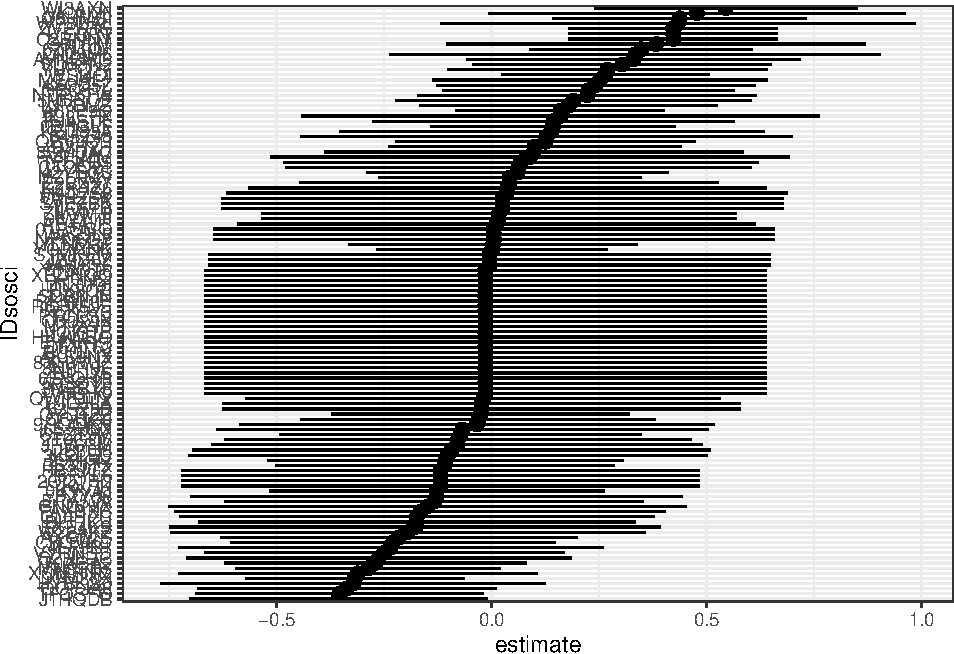
\includegraphics{workshop_panel_files/figure-latex/lmer-random-slope2-1.pdf}

\begin{itemize}
\item
  Mit jedem Punkt auf der Einstellungsskala steigt die Intention, sich mit anderen Personen außerhalb des Haushalts zu treffen, um ca. 0.4 Punkte.
\item
  Die Personen-spezifischen Effekte streuen mit einer Standardabweichung von ca. 0.3 Punkten um diesen durchschnittlichen Effekt durchaus wahrnehmbar. Die typischen Effekte (+/- 1 SD) liegen zwischen sehr geringen Effekten und deutlichen Effekten. Ein negativer Effekt der Einstellung auf die Intention ist selten.
\item
  Das Konfidenzintervall für die Standardabweichung des \emph{random slope} liegt deutlich über 0. Wir können davon ausgehen, dass es Heterogenität im Treatment-Effekt gibt. Manche Personen passen ihre Verhaltensintention ihren Einstellungen stärker an, bei anderen entwickeln sich Einstellung und Verhaltensintention weniger systematisch.
\item
  Der Likelihood-Ratio-Test und die Informationskriterien zeigen, dass das Modell mit \emph{random slope} wesentlich besser zu den Daten passt als das Modell nur mit \emph{random intercept}.
\item
  Die Abbildung vermittelt einen Eindruck von der Treatment-Effekt-Heterogenität. Dargestellt ist die die Abweichung vom durchschnittlichen Effekt (0.4). Neben der Verteilung sollten auch die weiten Intervalle beachtet werden. Auf Basis von nur vier Beobachtungen pro Person lassen sich die individuellen Abweichungen vom durchschnittlichen Effekt nur recht unpräzise quantifizieren.
\end{itemize}

\hypertarget{ebenen-uxfcberschreitende-interaktionen-cross-level-interactions}{%
\subsection*{Ebenen-überschreitende Interaktionen (cross-level interactions)}\label{ebenen-uxfcberschreitende-interaktionen-cross-level-interactions}}
\addcontentsline{toc}{subsection}{Ebenen-überschreitende Interaktionen (cross-level interactions)}

\begin{itemize}
\item
  \emph{Random slopes} zeigen nur eine allgemeine Heterogenität zwischen den Personen. Wir wissen nun, dass der Effekt der Einstellung auf das Verhalten bei verschiedenen Personen unterschiedlich ausfällt. Wir wissen aber nicht, an welchen Eigenschaften der Personen dies liegen könnte.
\item
  Wenn wir theoretisch von Effekt-Heterogenität ausgehen oder empirisch durch ein \emph{random slope} Modell Evidenz dafür gefunden haben, können wir in einem weiteren Schritt versuchen, diese Heterogenität zu erklären.
\item
  Dazu prüfen wir, ob eine Interaktion zwischen einem Personen-Merkmal und dem Prädiktor die allgemeine Heterogenität des Treatment-Effekts reduziert. Da das Personen-Merkmal auf Level 2 und der Prädiktor als über die Zeit variierende Variable auf Level 1 angesiedelt ist, spricht man hier auch von einer \emph{cross-level interaction}.
\item
  Im Beispiel wollen wir betrachten, ob die Berücksichtigung des Geschlechts einen Teil der Treatment-Effekt-Heterogenität erklären kann.

  \begin{itemize}
  \tightlist
  \item
    Dazu spezifizieren wir zwei weitere Modelle:

    \begin{itemize}
    \tightlist
    \item
      \texttt{m\_rs\_sex1} enthält den einfachen Haupteffekt des Geschlechts.
    \item
      \texttt{m\_rs\_sex2} enthält zudem die Interaktion zwischen der Einstellung und dem Geschlecht.
    \end{itemize}
  \end{itemize}
\end{itemize}

\begin{Shaded}
\begin{Highlighting}[]
\CommentTok{# Modell mit Random Slope als Referenz}
\NormalTok{m_rs =}\StringTok{ }\KeywordTok{lmer}\NormalTok{(verhint2 }\OperatorTok{~}\StringTok{ }\NormalTok{ein2 }\OperatorTok{+}\StringTok{ }\KeywordTok{factor}\NormalTok{(wave) }\OperatorTok{+}\StringTok{ }\NormalTok{(ein2 }\OperatorTok{|}\StringTok{ }\NormalTok{IDsosci), }\DataTypeTok{data =}\NormalTok{ d)}

\CommentTok{# Modell mit HE Geschlecht}
\NormalTok{m_rs_sex1 =}\StringTok{ }\KeywordTok{lmer}\NormalTok{(verhint2 }\OperatorTok{~}\StringTok{ }\NormalTok{ein2 }\OperatorTok{+}\StringTok{ }\NormalTok{C_sex }\OperatorTok{+}\StringTok{ }\KeywordTok{factor}\NormalTok{(wave) }\OperatorTok{+}\StringTok{ }\NormalTok{(ein2 }\OperatorTok{|}\StringTok{ }\NormalTok{IDsosci), }\DataTypeTok{data =}\NormalTok{ d)}
\NormalTok{m_rs_sex1 }\OperatorTok\StringTok{ }\KeywordTok{summary}\NormalTok{(}\DataTypeTok{correlation =} \OtherTok{FALSE}\NormalTok{)}
\end{Highlighting}
\end{Shaded}

\begin{verbatim}
## Linear mixed model fit by REML. t-tests use Satterthwaite's method [
## lmerModLmerTest]
## Formula: verhint2 ~ ein2 + C_sex + factor(wave) + (ein2 | IDsosci)
##    Data: d
## 
## REML criterion at convergence: 6221
## 
## Scaled residuals: 
##    Min     1Q Median     3Q    Max 
## -3.184 -0.424 -0.205  0.247  4.349 
## 
## Random effects:
##  Groups   Name        Variance Std.Dev. Corr 
##  IDsosci  (Intercept) 0.231    0.481         
##           ein2        0.112    0.334    -0.62
##  Residual             0.639    0.799         
## Number of obs: 2304, groups:  IDsosci, 576
## 
## Fixed effects:
##                 Estimate Std. Error         df t value     Pr(>|t|)    
## (Intercept)      0.82744    0.06062  758.00715   13.65      < 2e-16 ***
## ein2             0.40322    0.02696  371.85383   14.96      < 2e-16 ***
## C_sex           -0.00757    0.05279  386.27700   -0.14        0.886    
## factor(wave)2    0.11304    0.04829 1573.33025    2.34        0.019 *  
## factor(wave)3    0.19704    0.04834 1587.36240    4.08 0.0000480989 ***
## factor(wave)4    0.28810    0.04904 1646.41878    5.87 0.0000000051 ***
## ---
## Signif. codes:  0 '***' 0.001 '**' 0.01 '*' 0.05 '.' 0.1 ' ' 1
\end{verbatim}

\begin{Shaded}
\begin{Highlighting}[]
\CommentTok{# Modell mit IA Geschlecht*Einstellung}
\NormalTok{m_rs_sex2 =}\StringTok{ }\KeywordTok{lmer}\NormalTok{(verhint2 }\OperatorTok{~}\StringTok{ }\NormalTok{ein2 }\OperatorTok{*}\StringTok{ }\NormalTok{C_sex }\OperatorTok{+}\StringTok{ }\KeywordTok{factor}\NormalTok{(wave) }\OperatorTok{+}\StringTok{ }\NormalTok{(ein2 }\OperatorTok{|}\StringTok{ }\NormalTok{IDsosci), }\DataTypeTok{data =}\NormalTok{ d)}
\NormalTok{m_rs_sex2 }\OperatorTok\StringTok{ }\KeywordTok{summary}\NormalTok{(}\DataTypeTok{correlation =} \OtherTok{FALSE}\NormalTok{)}
\end{Highlighting}
\end{Shaded}

\begin{verbatim}
## Linear mixed model fit by REML. t-tests use Satterthwaite's method [
## lmerModLmerTest]
## Formula: verhint2 ~ ein2 * C_sex + factor(wave) + (ein2 | IDsosci)
##    Data: d
## 
## REML criterion at convergence: 6224
## 
## Scaled residuals: 
##    Min     1Q Median     3Q    Max 
## -3.190 -0.432 -0.213  0.244  4.340 
## 
## Random effects:
##  Groups   Name        Variance Std.Dev. Corr 
##  IDsosci  (Intercept) 0.230    0.480         
##           ein2        0.111    0.333    -0.62
##  Residual             0.639    0.799         
## Number of obs: 2304, groups:  IDsosci, 576
## 
## Fixed effects:
##                Estimate Std. Error        df t value Pr(>|t|)    
## (Intercept)      0.8733     0.0770  584.4186   11.34  < 2e-16 ***
## ein2             0.3702     0.0435  375.7244    8.51  4.1e-16 ***
## C_sex           -0.0811     0.0932  458.4467   -0.87     0.38    
## factor(wave)2    0.1128     0.0483 1573.3027    2.34     0.02 *  
## factor(wave)3    0.1973     0.0483 1587.2271    4.08  4.7e-05 ***
## factor(wave)4    0.2877     0.0490 1646.3174    5.87  5.3e-09 ***
## ein2:C_sex       0.0527     0.0551  367.9806    0.96     0.34    
## ---
## Signif. codes:  0 '***' 0.001 '**' 0.01 '*' 0.05 '.' 0.1 ' ' 1
## convergence code: 0
## Model failed to converge with max|grad| = 0.00291019 (tol = 0.002, component 1)
\end{verbatim}

\begin{Shaded}
\begin{Highlighting}[]
\CommentTok{# Wald-Test}
\KeywordTok{anova}\NormalTok{(m_rs, m_rs_sex1, m_rs_sex2)}
\end{Highlighting}
\end{Shaded}

\begin{verbatim}
## Data: d
## Models:
## m_rs: verhint2 ~ ein2 + factor(wave) + (ein2 | IDsosci)
## m_rs_sex1: verhint2 ~ ein2 + C_sex + factor(wave) + (ein2 | IDsosci)
## m_rs_sex2: verhint2 ~ ein2 * C_sex + factor(wave) + (ein2 | IDsosci)
##           Df  AIC  BIC logLik deviance Chisq Chi Df Pr(>Chisq)
## m_rs       9 6211 6262  -3096     6193                        
## m_rs_sex1 10 6213 6270  -3096     6193  0.02      1       0.89
## m_rs_sex2 11 6214 6277  -3096     6192  0.92      1       0.34
\end{verbatim}

\begin{Shaded}
\begin{Highlighting}[]
\CommentTok{# Reduktion der Varianz in random slope durch Interaktion}
\DecValTok{1} \OperatorTok{-}\StringTok{ }\NormalTok{(}\KeywordTok{as.numeric}\NormalTok{(}\KeywordTok{VarCorr}\NormalTok{(m_rs_sex2)}\OperatorTok{$}\NormalTok{IDsosci[}\StringTok{"ein2"}\NormalTok{, }\StringTok{"ein2"}\NormalTok{]}\OperatorTok{/}\KeywordTok{as.numeric}\NormalTok{(}\KeywordTok{VarCorr}\NormalTok{(m_rs_sex1)}\OperatorTok{$}\NormalTok{IDsosci[}\StringTok{"ein2"}\NormalTok{, }
    \StringTok{"ein2"}\NormalTok{])))}
\end{Highlighting}
\end{Shaded}

\begin{verbatim}
## [1] 0.0047
\end{verbatim}

\begin{itemize}
\tightlist
\item
  Das Geschlecht macht nur einen unwesentlichen Unterschied in der Intention, sich mit Personen außerhalb des Haushalts zu treffen, aus (\texttt{m\_rs\_sex1}).
\item
  Der Effekt der Einstellung auf die Intention unterscheidet sich kaum für Männer und Frauen (\texttt{m\_rs\_sex2}). Wichtig: In diesem Modell mit Interaktionseffekt haben die Koeffizienten der Prädiktoren eine andere Bedeutung als im Modell ohne Interaktionseffekt. Sie quantifizieren nicht mehr ``Haupteffekte'', sondern ``einfache'' Effekte (\emph{simple effects}). Der Koeffizient für \texttt{ein2} quantifiziert den Effekt, wenn \texttt{C\_sex} gleich 0 ist --- also den Effekt für Männer. Der Koeffizient des Interaktionsterms \texttt{ein2:C\_sex} quantifiziert den Unterschied im Effekt zwischen Männern und Frauen.
\item
  Der Likelihood-Ratio-Test und die Informationskriterien zeigen, dass weder die Aufnahme des Geschlechts noch die Interaktion der Einstellungen mit dem Geschlecht zur Verbesserung des Modells beitragen.
\item
  Durch den Vergleich der Varianz der \emph{random slopes} zwischen \texttt{m\_rs\_sex1} und \texttt{m\_rs\_sex2} können wir quantifizieren, welchen Anteil der Effekt-Heterogenität durch die Interaktion erklärt werden kann. In diesem Beispiel ist die Erklärungskraft der Interaktion zu vernachlässigen.
\item
  Ein ``erfolgreiches'' Modell mit \emph{random slopes} und \emph{cross-level interaction} findet ihr in der folgenden Übungsaufgabe.
\end{itemize}

\hypertarget{uxfcbungsaufgaben-5}{%
\section{Übungsaufgaben 5}\label{uxfcbungsaufgaben-5}}

\begin{enumerate}
\def\labelenumi{\arabic{enumi})}
\tightlist
\item
  Schätze den kausalen Effekt der Einstellung zum Verhalten, weniger als 1.5m Abstand zu Personen zu halten, die nicht im gleichen Haushalt leben \texttt{ein3}, auf die diesbezügliche Verhaltensintention (\texttt{verhint3}). Berücksichtige dabei die Periodeneffekte der Panelwellen. Siehe dazu auch Übung 4.

  \begin{itemize}
  \tightlist
  \item
    Schätze zuerst ein geeignetes Null-Modell mit \emph{random intercept} als Referenz.
  \item
    Schätze dann das \emph{random intercept} Panelmodell.
  \item
    Lasse den Effekt nun um den durchschnittlichen Effekt variieren. Prüfe, ob die Daten für Effekt-Heterogenität sprechen.
  \item
    Prüfe, ob sich der Effekt zwischen Personen ab 50 Jahren und Jüngeren unterscheidet. Wie stark kann das Berücksichtigen dieser Interaktion die Effekt-Heterogenität verringern?
  \end{itemize}
\item
  Spezifiziere, schätze und interpretiere ein eigenes \emph{random effects} Panelmodell mit \emph{random slope} und \emph{cross-level interaction} mit Daten aus dem Beispieldatensatz. Beachte dabei, dass wir hier an die Grenzen der Informationshaltigkeit der Daten für eine ML-Schätzung stoßen. Es ist recht wahrscheinlich, dass singuläre Fits oder nicht konvergierte Modelle vorkommen werden.
\end{enumerate}

\hypertarget{hybride-within-between-modelle}{%
\chapter{\texorpdfstring{Hybride \emph{within-between} Modelle}{Hybride within-between Modelle}}\label{hybride-within-between-modelle}}

\hypertarget{das-beste-aus-beiden-welten}{%
\section{Das Beste aus beiden Welten?}\label{das-beste-aus-beiden-welten}}

\begin{itemize}
\item
  Ein häufiger Einwand gegen \emph{random effects} Panelmodelle ist, dass die Annahme nicht korrelierter über die Zeit konstanter Variablen (beobachtet wie unbeobachtet) so stark ist, dass sie in den Sozialwissenschaften eigentlich nie einzuhalten ist (siehe Abschnitt 4.1).
\item
  Trotzdem sind \emph{random effects} Panelmodelle weit verbreitet, da sie uns erlauben, über die Zeit variierende Variablen und über die Zeit konstante Personenmerkmale als Prädiktoren in ein Modell aufzunehmen. Häufig sind wir eben sowohl an kausalen Effekten als auch an Unterschieden zwischen Personen interessiert.
\item
  Außerdem ist gerade die Möglichkeit, unspezifische Heterogenität in Treatment-Effekten zuzulassen, in den Sozialwissenschaften sehr attraktiv. Eigentlich gehen wir fast immer davon aus, dass Effekte variabel sind und nicht alle Personen gleichermaßen betreffen.
\item
  Das hybride \emph{within-between} Modell verspricht, unverzerrte kausale \emph{within-person} Effekte der über die Zeit variierenden Prädiktoren \emph{und} \emph{between-person} Vergleiche innerhalb eines Modells zu schätzen.
\item
  Dazu werden die über die Zeit variierenden Prädiktoren transformiert und in zwei Variablen aufgeteilt:

  \begin{itemize}
  \tightlist
  \item
    \(x_{it}-\bar{x_i}\) ist der um den Personen-Mittelwert bereinigte \emph{within-person} Prädiktor.
  \item
    \(\bar{x_i}\) ist der Personen-Mittelwert als \emph{between-person} Prädiktor.
  \end{itemize}
\item
  Der Koeffizient des \emph{within-person} Prädiktors entspricht dem \emph{fixed effects} Schätzer (siehe Abschnitt 3.1, Within Transformation). Der Koeffizient des \emph{between-person} Prädiktors quantifiziert die Unterschiede der Personen in \(y\), die durch über die Zeit stabile Unterschiede in \(x\) erklärt werden.
\item
  Ein Blick auf die Varianzaufklärung im ersten Beispiel zum \emph{random effects} Panelmodell in Abschnitt 4.5 zeigt, warum die Trennung dieser beiden Effekte sinnvoll ist. Das Ergebnis ist hier noch einmal reproduziert.
\end{itemize}

\begin{Shaded}
\begin{Highlighting}[]
\NormalTok{m1 }\OperatorTok\StringTok{ }\KeywordTok{summary}\NormalTok{(}\DataTypeTok{correlation =} \OtherTok{FALSE}\NormalTok{)}
\end{Highlighting}
\end{Shaded}

\begin{verbatim}
## Linear mixed model fit by REML. t-tests use Satterthwaite's method [
## lmerModLmerTest]
## Formula: verh1 ~ verhint1 + (1 | IDsosci)
##    Data: d
## 
## REML criterion at convergence: 4554
## 
## Scaled residuals: 
##    Min     1Q Median     3Q    Max 
## -4.524 -0.202 -0.085  0.165  5.793 
## 
## Random effects:
##  Groups   Name        Variance Std.Dev.
##  IDsosci  (Intercept) 0.111    0.334   
##  Residual             0.341    0.584   
## Number of obs: 2304, groups:  IDsosci, 576
## 
## Fixed effects:
##              Estimate Std. Error        df t value Pr(>|t|)    
## (Intercept)    0.5987     0.0287  975.4311    20.9   <2e-16 ***
## verhint1       0.5155     0.0122 1747.0982    42.3   <2e-16 ***
## ---
## Signif. codes:  0 '***' 0.001 '**' 0.01 '*' 0.05 '.' 0.1 ' ' 1
\end{verbatim}

\begin{Shaded}
\begin{Highlighting}[]
\KeywordTok{r2}\NormalTok{(m1, }\DataTypeTok{by_group =} \OtherTok{TRUE}\NormalTok{)}
\end{Highlighting}
\end{Shaded}

\begin{verbatim}
## # Explained Variance by Level
## 
## Level   |    R2
## ---------------
## Level 1 | 0.161
## IDsosci | 0.812
\end{verbatim}

\begin{itemize}
\tightlist
\item
  Die Verhaltensintention erklärt sowohl 81\% der Varianz zwischen den Personen als auch 16\% der Varianz innerhalb der Personen. Wir erhalten aber nur einen Koeffizienten, in dem der \emph{within-person} Effekt und der \emph{between-person} Unterschied untrennbar vermischt sind.
\end{itemize}

\hypertarget{spezifikation-des-within-between-modells}{%
\section{\texorpdfstring{Spezifikation des \emph{within-between} Modells}{Spezifikation des within-between Modells}}\label{spezifikation-des-within-between-modells}}

\hypertarget{within-between-modell-mit-random-intercept}{%
\subsection*{\texorpdfstring{\emph{within-between} Modell mit \emph{random intercept}}{within-between Modell mit random intercept}}\label{within-between-modell-mit-random-intercept}}
\addcontentsline{toc}{subsection}{\emph{within-between} Modell mit \emph{random intercept}}

\begin{itemize}
\item
  Wir untersuchen wieder den Effekt der Intention, die Wohnung ohne triftigen Grund zu verlassen, auf den Bericht, dies getan zu haben.
\item
  Zuerst transformieren wir den Prädiktor \texttt{verhint1} in einen \emph{within}-Prädiktor \texttt{verhint1\_w} und einen \emph{between}-Prädiktor \texttt{verhint1\_b}.
\end{itemize}

\begin{Shaded}
\begin{Highlighting}[]
\CommentTok{# Transformation: Trennen von within- und between-Prädiktor}
\NormalTok{d =}\StringTok{ }\NormalTok{d }\OperatorTok\StringTok{ }
\StringTok{  }\KeywordTok{group_by}\NormalTok{(IDsosci) }\OperatorTok\StringTok{ }
\StringTok{  }\KeywordTok{mutate}\NormalTok{(}\DataTypeTok{verhint1_w =}\NormalTok{ verhint1 }\OperatorTok{-}\StringTok{ }\KeywordTok{mean}\NormalTok{(verhint1), }\CommentTok{# within}
         \DataTypeTok{verhint1_b =} \KeywordTok{mean}\NormalTok{(verhint1)) }\OperatorTok\StringTok{ }\CommentTok{# between}
\StringTok{  }\KeywordTok{ungroup}\NormalTok{()}
\CommentTok{# Zwei Personen zur Illustration}
\NormalTok{d }\OperatorTok\StringTok{ }
\StringTok{  }\KeywordTok{filter}\NormalTok{(IDsosci }\OperatorTok\StringTok{ }\KeywordTok{c}\NormalTok{(}\StringTok{"050IPY"}\NormalTok{, }\StringTok{"02E6C8"}\NormalTok{)) }\OperatorTok\StringTok{ }
\StringTok{  }\KeywordTok{select}\NormalTok{(IDsosci, wave, }\KeywordTok{starts_with}\NormalTok{(}\StringTok{"verhint1"}\NormalTok{))}
\end{Highlighting}
\end{Shaded}

\begin{verbatim}
## # A tibble: 8 x 5
##   IDsosci  wave verhint1 verhint1_w verhint1_b
##   <chr>   <int>    <dbl>      <dbl>      <dbl>
## 1 02E6C8      1        1         -1          2
## 2 02E6C8      2        2          0          2
## 3 02E6C8      3        2          0          2
## 4 02E6C8      4        3          1          2
## 5 050IPY      1        3         -1          4
## 6 050IPY      2        3         -1          4
## 7 050IPY      3        5          1          4
## 8 050IPY      4        5          1          4
\end{verbatim}

\begin{itemize}
\item
  Am Beispiel von zwei Personen können wir sehen, dass \texttt{verhint1\_b} der Mittelwert der Person über die vier Wellen ist und \texttt{verhint1\_w} der Messwert in einer Welle bereinigt um den Mittelwert. Es wird auch direkt deutlich, dass \texttt{verhint1\_b} nun per Transformationslogik eine über die Zeit konstante Personeneigenschaft ist.
\item
  Die Spezifikation des Modells mit \texttt{lme4::lmer()} folgt derselben Logik wie das \emph{random effects} Panelmodell in Abschnitt 4.

  \begin{itemize}
  \tightlist
  \item
    Als Referenz ziehen wir das entsprechende Null-Modell inklusive der \emph{fixed effects} für die Panelwellen heran.
  \item
    Wir beginnen wieder mit einem \emph{random intercept} Modell, \texttt{(1\ \textbar{}\ IDsosci)}.
  \item
    \texttt{verhint1\_w} und \texttt{verhint1\_b} werden als Prädiktoren in das Modell aufgenommen.
  \end{itemize}
\end{itemize}

\begin{Shaded}
\begin{Highlighting}[]
\CommentTok{# Null-Modell als Referenz}
\NormalTok{wb_}\DecValTok{0}\NormalTok{ =}\StringTok{ }\KeywordTok{lmer}\NormalTok{(verh1 }\OperatorTok{~}\StringTok{ }\DecValTok{1} \OperatorTok{+}\StringTok{ }\KeywordTok{factor}\NormalTok{(wave) }\OperatorTok{+}\StringTok{ }\NormalTok{(}\DecValTok{1} \OperatorTok{|}\StringTok{ }\NormalTok{IDsosci), }\DataTypeTok{data =}\NormalTok{ d)}

\CommentTok{# Within-between Modell mit random intercept}
\NormalTok{wb_ri =}\StringTok{ }\KeywordTok{lmer}\NormalTok{(verh1 }\OperatorTok{~}\StringTok{ }\NormalTok{verhint1_w }\OperatorTok{+}\StringTok{ }\NormalTok{verhint1_b }\OperatorTok{+}\StringTok{ }\KeywordTok{factor}\NormalTok{(wave) }\OperatorTok{+}\StringTok{ }\NormalTok{(}\DecValTok{1} \OperatorTok{|}\StringTok{ }\NormalTok{IDsosci), }\DataTypeTok{data =}\NormalTok{ d)}
\NormalTok{wb_ri }\OperatorTok\StringTok{ }\KeywordTok{summary}\NormalTok{(}\DataTypeTok{correlation =} \OtherTok{FALSE}\NormalTok{)}
\end{Highlighting}
\end{Shaded}

\begin{verbatim}
## Linear mixed model fit by REML. t-tests use Satterthwaite's method [
## lmerModLmerTest]
## Formula: verh1 ~ verhint1_w + verhint1_b + factor(wave) + (1 | IDsosci)
##    Data: d
## 
## REML criterion at convergence: 4303
## 
## Scaled residuals: 
##    Min     1Q Median     3Q    Max 
## -5.289 -0.318 -0.044  0.166  6.372 
## 
## Random effects:
##  Groups   Name        Variance Std.Dev.
##  IDsosci  (Intercept) 0.0755   0.275   
##  Residual             0.3165   0.563   
## Number of obs: 2304, groups:  IDsosci, 576
## 
## Fixed effects:
##                Estimate Std. Error        df t value Pr(>|t|)    
## (Intercept)      0.1689     0.0392 1069.4869    4.31 0.000018 ***
## verhint1_w       0.3288     0.0166 1724.0000   19.79  < 2e-16 ***
## verhint1_b       0.7153     0.0159  574.0000   44.86  < 2e-16 ***
## factor(wave)2    0.0200     0.0336 1724.0000    0.60  0.55169    
## factor(wave)3    0.1400     0.0337 1724.0000    4.15 0.000034 ***
## factor(wave)4    0.1178     0.0345 1724.0000    3.41  0.00065 ***
## ---
## Signif. codes:  0 '***' 0.001 '**' 0.01 '*' 0.05 '.' 0.1 ' ' 1
\end{verbatim}

\begin{Shaded}
\begin{Highlighting}[]
\CommentTok{# Varianzreduktion}
\DecValTok{1} \OperatorTok{-}\StringTok{ }\NormalTok{(}\KeywordTok{sigma}\NormalTok{(wb_ri)}\OperatorTok{^}\DecValTok{2}\OperatorTok{/}\KeywordTok{sigma}\NormalTok{(wb_}\DecValTok{0}\NormalTok{)}\OperatorTok{^}\DecValTok{2}\NormalTok{)  }\CommentTok{# L1}
\end{Highlighting}
\end{Shaded}

\begin{verbatim}
## [1] 0.18
\end{verbatim}

\begin{Shaded}
\begin{Highlighting}[]
\DecValTok{1} \OperatorTok{-}\StringTok{ }\NormalTok{(}\KeywordTok{as.numeric}\NormalTok{(}\KeywordTok{VarCorr}\NormalTok{(wb_ri)}\OperatorTok{$}\NormalTok{IDsosci)}\OperatorTok{/}\KeywordTok{as.numeric}\NormalTok{(}\KeywordTok{VarCorr}\NormalTok{(wb_}\DecValTok{0}\NormalTok{)}\OperatorTok{$}\NormalTok{IDsosci))  }\CommentTok{# L2}
\end{Highlighting}
\end{Shaded}

\begin{verbatim}
## [1] 0.87
\end{verbatim}

\begin{Shaded}
\begin{Highlighting}[]
\CommentTok{# Vergleich mit fixed effects Modell}
\KeywordTok{plm}\NormalTok{(verh1 }\OperatorTok{~}\StringTok{ }\NormalTok{verhint1 }\OperatorTok{+}\StringTok{ }\KeywordTok{factor}\NormalTok{(wave), }\DataTypeTok{data =}\NormalTok{ d, }\DataTypeTok{index =} \StringTok{"IDsosci"}\NormalTok{, }\DataTypeTok{model =} \StringTok{"within"}\NormalTok{) }\OperatorTok\StringTok{ }
\StringTok{    }\KeywordTok{summary}\NormalTok{() }\OperatorTok\StringTok{ }\KeywordTok{coef}\NormalTok{()}
\end{Highlighting}
\end{Shaded}

\begin{verbatim}
##               Estimate Std. Error t-value Pr(>|t|)
## verhint1          0.33      0.017    19.8  1.0e-78
## factor(wave)2     0.02      0.034     0.6  5.5e-01
## factor(wave)3     0.14      0.034     4.2  3.4e-05
## factor(wave)4     0.12      0.034     3.4  6.5e-04
\end{verbatim}

\begin{itemize}
\tightlist
\item
  Kausaler Effekt: Wenn die Intention um einen Punkt steigt, dann wird das Verhalten um 0.3 Punkte häufiger. Der Effekt erklärt 18\% der Varianz innerhalb der Personen.

  \begin{itemize}
  \tightlist
  \item
    Der Koeffizient des \emph{within}-Prädiktors entspricht genau dem Koeffizienten eines klassischen \emph{fixed effects} Modell, wie wir es z.B. mit \texttt{plm} geschätzt haben.
  \end{itemize}
\item
  Unterschiede zwischen Personen: Zwei Personen, deren durchschnittliche Intention sich um einen Punkt unterscheidet, unterscheiden sich um 0.7 Punkte in ihrer mittleren Häufigkeit, das Haus ohne triftigen Grund zu verlassen. Dieser Zusammenhang erklärt 87\% der Varianz zwischen den Personen.
\end{itemize}

\hypertarget{within-between-modell-mit-random-slope-und-cross-level-interaktion}{%
\subsection*{\texorpdfstring{\emph{within-between} Modell mit \emph{random slope} und \emph{cross-level} Interaktion}{within-between Modell mit random slope und cross-level Interaktion}}\label{within-between-modell-mit-random-slope-und-cross-level-interaktion}}
\addcontentsline{toc}{subsection}{\emph{within-between} Modell mit \emph{random slope} und \emph{cross-level} Interaktion}

\begin{itemize}
\tightlist
\item
  Im \emph{within-between} Modell können wir den Koeffizienten des \emph{within}-Prädiktors zwischen den Personen variieren lassen. Dadurch lassen wir Heterogenität um den durchschnittlichen Treatment-Effekt zu. In der Formel ergänzen wir \texttt{(verhint\_w\ \textbar{}\ IDsosci)}

  \begin{itemize}
  \tightlist
  \item
    \citet{bellFixedRandomEffects2019} empfehlen, im Idealfall die Koeffizienten aller, zumindest aber die der wichtigsten \emph{within}-Prädiktoren zwischen den Personen variieren zu lassen.
  \end{itemize}
\item
  In der Folge können wir testen, auf welche Personenmerkmale sich die unspezifische Heterogenität zurückführen lässt. Hier prüfen wir, ob der kausale Effekt sich nach dem Geschlecht unterscheidet: \texttt{verhint1\_w\ *\ C\_sex}.
\end{itemize}

\begin{Shaded}
\begin{Highlighting}[]
\CommentTok{# Random slope für within-Effekt}
\NormalTok{wb_rs =}\StringTok{ }\KeywordTok{lmer}\NormalTok{(verh1 }\OperatorTok{~}\StringTok{ }\NormalTok{verhint1_w }\OperatorTok{+}\StringTok{ }\NormalTok{verhint1_b }\OperatorTok{+}\StringTok{ }\KeywordTok{factor}\NormalTok{(wave) }\OperatorTok{+}\StringTok{ }\NormalTok{(verhint1_w }\OperatorTok{|}\StringTok{ }\NormalTok{IDsosci), }
    \DataTypeTok{data =}\NormalTok{ d)}
\NormalTok{wb_rs }\OperatorTok\StringTok{ }\KeywordTok{summary}\NormalTok{(}\DataTypeTok{correlation =} \OtherTok{FALSE}\NormalTok{)}
\end{Highlighting}
\end{Shaded}

\begin{verbatim}
## Linear mixed model fit by REML. t-tests use Satterthwaite's method [
## lmerModLmerTest]
## Formula: verh1 ~ verhint1_w + verhint1_b + factor(wave) + (verhint1_w |  
##     IDsosci)
##    Data: d
## 
## REML criterion at convergence: 4057
## 
## Scaled residuals: 
##    Min     1Q Median     3Q    Max 
## -6.003 -0.334 -0.068  0.130  7.005 
## 
## Random effects:
##  Groups   Name        Variance Std.Dev. Corr
##  IDsosci  (Intercept) 0.0942   0.307        
##           verhint1_w  0.0968   0.311    0.63
##  Residual             0.2429   0.493        
## Number of obs: 2304, groups:  IDsosci, 576
## 
## Fixed effects:
##                 Estimate Std. Error         df t value     Pr(>|t|)    
## (Intercept)      0.21851    0.03766 1037.67349    5.80 0.0000000087 ***
## verhint1_w       0.40642    0.02469  295.92758   16.46      < 2e-16 ***
## verhint1_b       0.69774    0.01556  605.59516   44.85      < 2e-16 ***
## factor(wave)2    0.00409    0.03043 1616.73231    0.13      0.89316    
## factor(wave)3    0.10461    0.03056 1620.45144    3.42      0.00063 ***
## factor(wave)4    0.09744    0.03159 1654.47637    3.09      0.00207 ** 
## ---
## Signif. codes:  0 '***' 0.001 '**' 0.01 '*' 0.05 '.' 0.1 ' ' 1
\end{verbatim}

\begin{Shaded}
\begin{Highlighting}[]
\CommentTok{# Modellvergleich}
\KeywordTok{anova}\NormalTok{(wb_ri, wb_rs)}
\end{Highlighting}
\end{Shaded}

\begin{verbatim}
## Data: d
## Models:
## wb_ri: verh1 ~ verhint1_w + verhint1_b + factor(wave) + (1 | IDsosci)
## wb_rs: verh1 ~ verhint1_w + verhint1_b + factor(wave) + (verhint1_w | 
## wb_rs:     IDsosci)
##       Df  AIC  BIC logLik deviance Chisq Chi Df Pr(>Chisq)    
## wb_ri  8 4284 4330  -2134     4268                            
## wb_rs 10 4042 4100  -2011     4022   246      2     <2e-16 ***
## ---
## Signif. codes:  0 '***' 0.001 '**' 0.01 '*' 0.05 '.' 0.1 ' ' 1
\end{verbatim}

\begin{Shaded}
\begin{Highlighting}[]
\CommentTok{# Interaktion des within-Prädiktors mit Geschlecht}
\NormalTok{wb_rs_ia =}\StringTok{ }\KeywordTok{lmer}\NormalTok{(verh1 }\OperatorTok{~}\StringTok{ }\NormalTok{verhint1_w }\OperatorTok{*}\StringTok{ }\NormalTok{C_sex }\OperatorTok{+}\StringTok{ }\NormalTok{verhint1_b }\OperatorTok{+}\StringTok{ }\KeywordTok{factor}\NormalTok{(wave) }\OperatorTok{+}\StringTok{ }\NormalTok{(verhint1_w }\OperatorTok{|}\StringTok{ }
\StringTok{    }\NormalTok{IDsosci), }\DataTypeTok{data =}\NormalTok{ d)}
\NormalTok{wb_rs_ia }\OperatorTok\StringTok{ }\KeywordTok{summary}\NormalTok{(}\DataTypeTok{correlation =} \OtherTok{FALSE}\NormalTok{)}
\end{Highlighting}
\end{Shaded}

\begin{verbatim}
## Linear mixed model fit by REML. t-tests use Satterthwaite's method [
## lmerModLmerTest]
## Formula: 
## verh1 ~ verhint1_w * C_sex + verhint1_b + factor(wave) + (verhint1_w |  
##     IDsosci)
##    Data: d
## 
## REML criterion at convergence: 4062
## 
## Scaled residuals: 
##    Min     1Q Median     3Q    Max 
## -5.975 -0.338 -0.049  0.149  7.028 
## 
## Random effects:
##  Groups   Name        Variance Std.Dev. Corr
##  IDsosci  (Intercept) 0.0935   0.306        
##           verhint1_w  0.0973   0.312    0.63
##  Residual             0.2428   0.493        
## Number of obs: 2304, groups:  IDsosci, 576
## 
## Fixed effects:
##                    Estimate Std. Error         df t value     Pr(>|t|)    
## (Intercept)         0.26512    0.04446  876.66346    5.96 0.0000000036 ***
## verhint1_w          0.43310    0.03847  280.85689   11.26      < 2e-16 ***
## C_sex              -0.06732    0.03377  571.52249   -1.99      0.04664 *  
## verhint1_b          0.69476    0.01563  604.19894   44.44      < 2e-16 ***
## factor(wave)2       0.00402    0.03043 1616.08075    0.13      0.89483    
## factor(wave)3       0.10435    0.03056 1619.50527    3.41      0.00065 ***
## factor(wave)4       0.09741    0.03158 1653.82795    3.08      0.00207 ** 
## verhint1_w:C_sex   -0.04512    0.04882  272.73255   -0.92      0.35619    
## ---
## Signif. codes:  0 '***' 0.001 '**' 0.01 '*' 0.05 '.' 0.1 ' ' 1
\end{verbatim}

\begin{Shaded}
\begin{Highlighting}[]
\CommentTok{# Modellvergleich}
\KeywordTok{anova}\NormalTok{(wb_ri, wb_rs, wb_rs_ia)}
\end{Highlighting}
\end{Shaded}

\begin{verbatim}
## Data: d
## Models:
## wb_ri: verh1 ~ verhint1_w + verhint1_b + factor(wave) + (1 | IDsosci)
## wb_rs: verh1 ~ verhint1_w + verhint1_b + factor(wave) + (verhint1_w | 
## wb_rs:     IDsosci)
## wb_rs_ia: verh1 ~ verhint1_w * C_sex + verhint1_b + factor(wave) + (verhint1_w | 
## wb_rs_ia:     IDsosci)
##          Df  AIC  BIC logLik deviance  Chisq Chi Df Pr(>Chisq)    
## wb_ri     8 4284 4330  -2134     4268                             
## wb_rs    10 4042 4100  -2011     4022 245.62      2     <2e-16 ***
## wb_rs_ia 12 4042 4111  -2009     4018   4.15      2       0.13    
## ---
## Signif. codes:  0 '***' 0.001 '**' 0.01 '*' 0.05 '.' 0.1 ' ' 1
\end{verbatim}

\begin{Shaded}
\begin{Highlighting}[]
\CommentTok{# Reduktion der Varianz in random slope durch Interaktion}
\DecValTok{1} \OperatorTok{-}\StringTok{ }\NormalTok{(}\KeywordTok{as.numeric}\NormalTok{(}\KeywordTok{VarCorr}\NormalTok{(wb_rs_ia)}\OperatorTok{$}\NormalTok{IDsosci[}\StringTok{"verhint1_w"}\NormalTok{, }\StringTok{"verhint1_w"}\NormalTok{]}\OperatorTok{/}\KeywordTok{as.numeric}\NormalTok{(}\KeywordTok{VarCorr}\NormalTok{(wb_rs)}\OperatorTok{$}\NormalTok{IDsosci[}\StringTok{"verhint1_w"}\NormalTok{, }
    \StringTok{"verhint1_w"}\NormalTok{])))}
\end{Highlighting}
\end{Shaded}

\begin{verbatim}
## [1] -0.0049
\end{verbatim}

\begin{itemize}
\tightlist
\item
  Es gibt substantiell bedeutsame, statistisch signifikante Heterogenität um den durchschnittlichen Effekt der Intention auf das Verhalten.

  \begin{itemize}
  \tightlist
  \item
    Der durchschnittliche kausale \emph{within}-Effekt und der Unterschied zwischen den Personen bleiben substantiell unverändert.
  \item
    Die typischen Effekte (\emph{fixed effect} von \texttt{verhint1\_w} \(\pm 1 SD\)) schwanken zwischen kleinen und deutlichen Effekten.
  \item
    Die Aufnahme des \emph{random slope} verbessert das Modell nach allen Kriterien deutlich.
  \end{itemize}
\item
  Der kausale Effekt ist nicht wesentlich vom Geschlecht abhängig. Er fällt für Frauen unwesentlich und nicht statistisch signifikant schwächer aus als für Männer.

  \begin{itemize}
  \tightlist
  \item
    Die Standardabweichung des \emph{random slope} aus dem Modell ohne Interaktion hilft, die Effektstärke der Interaktion einzuordnen. Die mittlere Abweichung vom durchschnittlichen Effekt beträgt 0.3 Punkte. Die Effekte für Frauen und Männer unterscheiden sich um 0.04 Punkte. Gemessen an der Gesamt-Heterogenität ist die Heterogenität zwischen den Geschlechtern zu vernachlässigen. Dies zeigt sich auch an der (nicht existenten) Reduktion der Varianz im \emph{random slope}.
  \end{itemize}
\end{itemize}

\hypertarget{spezialfall-interaktion-von-within--und-between-pruxe4diktor}{%
\subsection*{\texorpdfstring{Spezialfall: Interaktion von \emph{within}- und \emph{between}-Prädiktor}{Spezialfall: Interaktion von within- und between-Prädiktor}}\label{spezialfall-interaktion-von-within--und-between-pruxe4diktor}}
\addcontentsline{toc}{subsection}{Spezialfall: Interaktion von \emph{within}- und \emph{between}-Prädiktor}

\begin{itemize}
\tightlist
\item
  Eine Interaktion des \emph{within}- mit dem \emph{between}-Prädiktor erlaubt es zu untersuchen, ob sich der kausale Effekt eines Prädiktors in Abhängigkeit der durchschnittlichen Ausprägung unterscheidet. Im vorliegenden Beispiel können wir testen, ob sich die Verhaltensintention stärker bei den Personen zu einer Handlung führt, die allgemein eher vorhaben, diese Handlung auszuüben.
\item
  Um die Koeffizienten in einem Modell mit einem Interaktionsterm aus zwei kontinuierlichen Variablen besser interpretierbar zu machen, zentrieren wir den \emph{between}-Prädiktor um seinen Mittelwert. Der Mittelwert des \emph{within}-Prädiktors ist durch die \emph{within}-Transformation bereits gleich 0.
\end{itemize}

\begin{Shaded}
\begin{Highlighting}[]
\CommentTok{# Zentrieren des between-Prädiktors}
\NormalTok{d =}\StringTok{ }\NormalTok{d }\OperatorTok\StringTok{ }\KeywordTok{mutate}\NormalTok{(}\DataTypeTok{verhint1_bc =}\NormalTok{ verhint1_b }\OperatorTok{-}\StringTok{ }\KeywordTok{mean}\NormalTok{(verhint1_b))}

\CommentTok{# Interaktion von within- und between Prädiktor}
\NormalTok{wb_rs_iawb =}\StringTok{ }\KeywordTok{lmer}\NormalTok{(verh1 }\OperatorTok{~}\StringTok{ }\NormalTok{verhint1_w }\OperatorTok{*}\StringTok{ }\NormalTok{verhint1_bc }\OperatorTok{+}\StringTok{ }\KeywordTok{factor}\NormalTok{(wave) }\OperatorTok{+}\StringTok{ }\NormalTok{(verhint1_w }\OperatorTok{|}\StringTok{ }
\StringTok{    }\NormalTok{IDsosci), }\DataTypeTok{data =}\NormalTok{ d)}
\NormalTok{wb_rs_iawb }\OperatorTok\StringTok{ }\KeywordTok{summary}\NormalTok{(}\DataTypeTok{correlation =} \OtherTok{FALSE}\NormalTok{)}
\end{Highlighting}
\end{Shaded}

\begin{verbatim}
## Linear mixed model fit by REML. t-tests use Satterthwaite's method [
## lmerModLmerTest]
## Formula: verh1 ~ verhint1_w * verhint1_bc + factor(wave) + (verhint1_w |  
##     IDsosci)
##    Data: d
## 
## REML criterion at convergence: 4037
## 
## Scaled residuals: 
##    Min     1Q Median     3Q    Max 
## -6.056 -0.374 -0.062  0.144  7.028 
## 
## Random effects:
##  Groups   Name        Variance Std.Dev. Corr
##  IDsosci  (Intercept) 0.0940   0.307        
##           verhint1_w  0.0864   0.294    0.66
##  Residual             0.2423   0.492        
## Number of obs: 2304, groups:  IDsosci, 576
## 
## Fixed effects:
##                          Estimate Std. Error         df t value   Pr(>|t|)    
## (Intercept)               1.47593    0.02509 1933.84933   58.82    < 2e-16 ***
## verhint1_w                0.32919    0.02825  400.16941   11.65    < 2e-16 ***
## verhint1_bc               0.71534    0.01594  574.00586   44.86    < 2e-16 ***
## factor(wave)2             0.00342    0.03033 1626.70386    0.11    0.91014    
## factor(wave)3             0.10593    0.03045 1631.33777    3.48    0.00052 ***
## factor(wave)4             0.10152    0.03146 1664.84967    3.23    0.00128 ** 
## verhint1_w:verhint1_bc    0.13744    0.02701  345.59075    5.09 0.00000059 ***
## ---
## Signif. codes:  0 '***' 0.001 '**' 0.01 '*' 0.05 '.' 0.1 ' ' 1
\end{verbatim}

\begin{Shaded}
\begin{Highlighting}[]
\CommentTok{# Reduktion der Varianz in random slope durch Interaktion}
\DecValTok{1} \OperatorTok{-}\StringTok{ }\NormalTok{(}\KeywordTok{as.numeric}\NormalTok{(}\KeywordTok{VarCorr}\NormalTok{(wb_rs_iawb)}\OperatorTok{$}\NormalTok{IDsosci[}\StringTok{"verhint1_w"}\NormalTok{, }\StringTok{"verhint1_w"}\NormalTok{]}\OperatorTok{/}\KeywordTok{as.numeric}\NormalTok{(}\KeywordTok{VarCorr}\NormalTok{(wb_rs)}\OperatorTok{$}\NormalTok{IDsosci[}\StringTok{"verhint1_w"}\NormalTok{, }
    \StringTok{"verhint1_w"}\NormalTok{])))}
\end{Highlighting}
\end{Shaded}

\begin{verbatim}
## [1] 0.11
\end{verbatim}

\begin{Shaded}
\begin{Highlighting}[]
\CommentTok{# Plot des kausalen Effekts als Funktion des between-Prädiktors}
\KeywordTok{tibble}\NormalTok{(}\DataTypeTok{b1 =} \KeywordTok{fixef}\NormalTok{(wb_rs_iawb)[}\StringTok{"verhint1_w"}\NormalTok{], }\DataTypeTok{b3 =} \KeywordTok{fixef}\NormalTok{(wb_rs_iawb)[}\StringTok{"verhint1_w:verhint1_bc"}\NormalTok{], }
    \DataTypeTok{Z =} \KeywordTok{quantile}\NormalTok{(}\KeywordTok{model.frame}\NormalTok{(wb_rs_iawb)[, }\StringTok{"verhint1_bc"}\NormalTok{], }\DataTypeTok{probs =}\NormalTok{ (}\DecValTok{0}\OperatorTok{:}\DecValTok{10}\NormalTok{)}\OperatorTok{/}\DecValTok{10}\NormalTok{), }\DataTypeTok{theta =}\NormalTok{ b1 }\OperatorTok{+}\StringTok{ }
\StringTok{        }\NormalTok{Z }\OperatorTok{*}\StringTok{ }\NormalTok{b3, }\DataTypeTok{se_b1 =} \KeywordTok{coef}\NormalTok{(}\KeywordTok{summary}\NormalTok{(wb_rs_iawb))[}\StringTok{"verhint1_w"}\NormalTok{, }\DecValTok{2}\NormalTok{], }\DataTypeTok{COV_b1b3 =} \KeywordTok{vcov}\NormalTok{(wb_rs_iawb)[}\StringTok{"verhint1_w"}\NormalTok{, }
        \StringTok{"verhint1_w:verhint1_bc"}\NormalTok{], }\DataTypeTok{se_b3 =} \KeywordTok{coef}\NormalTok{(}\KeywordTok{summary}\NormalTok{(wb_rs_iawb))[}\StringTok{"verhint1_w:verhint1_bc"}\NormalTok{, }
        \DecValTok{2}\NormalTok{], }\DataTypeTok{se_theta =} \KeywordTok{sqrt}\NormalTok{(se_b1}\OperatorTok{^}\DecValTok{2} \OperatorTok{+}\StringTok{ }\DecValTok{2} \OperatorTok{*}\StringTok{ }\NormalTok{Z }\OperatorTok{*}\StringTok{ }\NormalTok{COV_b1b3 }\OperatorTok{+}\StringTok{ }\NormalTok{Z}\OperatorTok{^}\DecValTok{2} \OperatorTok{*}\StringTok{ }\NormalTok{se_b3}\OperatorTok{^}\DecValTok{2}\NormalTok{), }\DataTypeTok{ci.lo_theta =}\NormalTok{ theta }\OperatorTok{+}\StringTok{ }
\StringTok{        }\KeywordTok{qt}\NormalTok{(}\FloatTok{0.05}\OperatorTok{/}\DecValTok{2}\NormalTok{, }\KeywordTok{df.residual}\NormalTok{(wb_rs_iawb)) }\OperatorTok{*}\StringTok{ }\NormalTok{se_theta, }\DataTypeTok{ci.hi_theta =}\NormalTok{ theta }\OperatorTok{+}\StringTok{ }\KeywordTok{qt}\NormalTok{(}\DecValTok{1} \OperatorTok{-}\StringTok{ }
\StringTok{        }\FloatTok{0.05}\OperatorTok{/}\DecValTok{2}\NormalTok{, }\KeywordTok{df.residual}\NormalTok{(wb_rs_iawb)) }\OperatorTok{*}\StringTok{ }\NormalTok{se_theta) }\OperatorTok\StringTok{ }\KeywordTok{ggplot}\NormalTok{(}\KeywordTok{aes}\NormalTok{(Z, theta, }\DataTypeTok{ymin =}\NormalTok{ ci.lo_theta, }
    \DataTypeTok{ymax =}\NormalTok{ ci.hi_theta)) }\OperatorTok{+}\StringTok{ }\KeywordTok{geom_ribbon}\NormalTok{(}\DataTypeTok{alpha =} \FloatTok{0.2}\NormalTok{) }\OperatorTok{+}\StringTok{ }\KeywordTok{geom_line}\NormalTok{() }\OperatorTok{+}\StringTok{ }\KeywordTok{geom_rug}\NormalTok{(}\DataTypeTok{data =} \KeywordTok{filter}\NormalTok{(d, }
\NormalTok{    wave }\OperatorTok{==}\StringTok{ }\DecValTok{1}\NormalTok{), }\KeywordTok{aes}\NormalTok{(verhint1_bc, }\DecValTok{0}\NormalTok{), }\DataTypeTok{sides =} \StringTok{"b"}\NormalTok{, }\DataTypeTok{inherit.aes =}\NormalTok{ F, }\DataTypeTok{position =} \KeywordTok{position_jitter}\NormalTok{(}\DataTypeTok{width =} \FloatTok{0.1}\NormalTok{, }
    \DataTypeTok{height =} \DecValTok{0}\NormalTok{), }\DataTypeTok{alpha =} \FloatTok{0.2}\NormalTok{, }\DataTypeTok{length =} \KeywordTok{unit}\NormalTok{(}\DecValTok{1}\NormalTok{, }\StringTok{"cm"}\NormalTok{)) }\OperatorTok{+}\StringTok{ }\KeywordTok{labs}\NormalTok{(}\DataTypeTok{x =} \StringTok{"Verhaltensintention Between (zentriert)"}\NormalTok{, }
    \DataTypeTok{y =} \StringTok{" Within-Effekt der Verhaltensintention"}\NormalTok{)}
\end{Highlighting}
\end{Shaded}

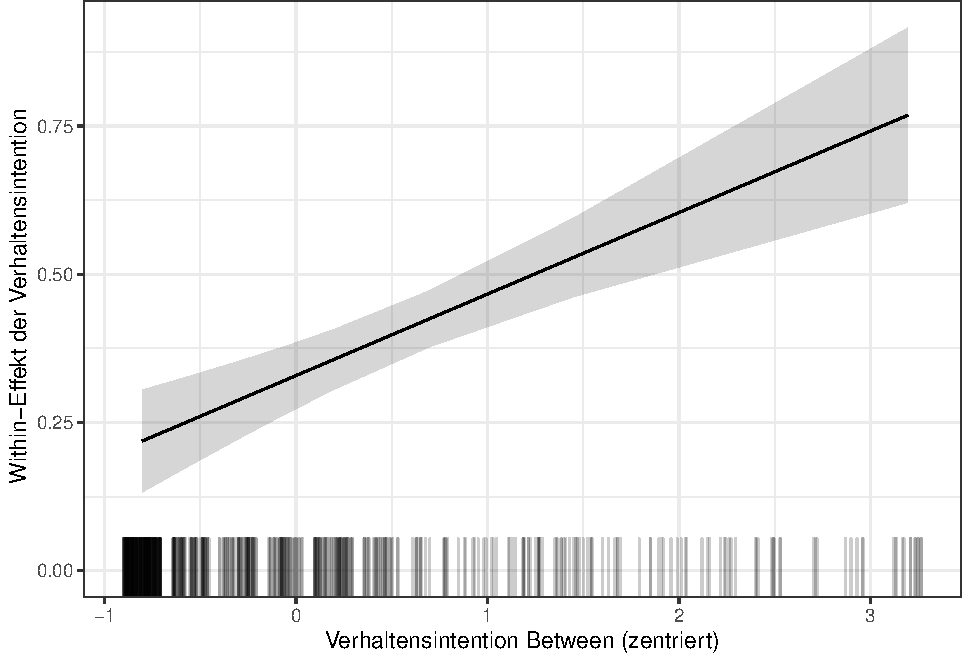
\includegraphics{workshop_panel_files/figure-latex/wb3-1.pdf}

\begin{itemize}
\tightlist
\item
  \texttt{verhint1\_w}: Der kausale \emph{within}-Effekt für Personen, \emph{deren mittlere Verhaltensintention dem Stichprobenmittelwert entspricht}, beträgt 0.3 Punkte.
\item
  \texttt{verhint1\_b}: Zwei Personen, deren mittlere Verhaltensintention sich um einen Punkt unterscheidet, unterscheiden sich \emph{dann, wenn ihre aktuelle Verhaltensintention ihrer mittleren Verhaltensintention entspricht}, um 0.7 Punkte.
\item
  \texttt{verhint1\_w:verhint1\_bc}: Der kausale Effekt unterscheidet sich zwischen zwei Personen, deren mittlere Verhaltensintention sich um einen Punkt unterscheidet, um 0.1 Punkte. Die Interaktion verringert die Varianz im \emph{random slope} um 11\%.

  \begin{itemize}
  \tightlist
  \item
    Wie sich der kausale Effekt in Abhängigkeit der mittleren Verhaltensintention verändert, ist in der Abbildung dargestellt. Die ``Barcodes'' am unteren Rand zeigen die Verteilung des \emph{between}-Prädiktors in der Stichprobe. Die graue Fläche um die Linie ist ein 95\%-Konfidenzintervall.
  \item
    Bei Personen, die über die Wellen hinweg eine größere Intention zeigen (= auf \emph{between}-Prädiktor höhere Werte haben), führt eine Steigerung der Intention zu einer deutlicheren Steigerung der Handlungshäufigkeit. Bei Personen, die insgesamt nur eine geringe Intention haben, nach draußen zu gehen (die deutliche Mehrheit in der Stichprobe), ist der kausale Effekt schwächer ausgeprägt.
  \end{itemize}
\end{itemize}

\hypertarget{zusammenfassung}{%
\subsection*{Zusammenfassung}\label{zusammenfassung}}
\addcontentsline{toc}{subsection}{Zusammenfassung}

\begin{quote}
We hope the discussion above has convinced readers of the superiority of the REWB model, except perhaps when the within and between effects are approximately equal, in which case the standard RE model (without separated within and between effects) might be preferable for reasons of efficiency. Even then, the REWB model should be considered first, or as an alternative, since the equality of the within and between coefficients should not be assumed. As for FE, except for simplicity there is nothing that such models offer that a REWB model does not. --- \citet{bellFixedRandomEffects2019}
\end{quote}

\hypertarget{uxfcbungsaufgaben-6}{%
\section{Übungsaufgaben 6}\label{uxfcbungsaufgaben-6}}

\begin{enumerate}
\def\labelenumi{\arabic{enumi})}
\tightlist
\item
  Schätze den kausalen Effekt der Einstellung \texttt{ein3} und der wahrgenommenen deskriptiven Norm \texttt{desnormp3} mit Bezug zum Einhalten des Abstands von 1.5m zu anderen Personen auf die Intention, diese Verhaltensregel zu befolgen. Untersuche auch den Zusammenhang zwischen den über die Zeit stabilen Anteilen der Prädiktoren und dem Kriterium.

  \begin{itemize}
  \tightlist
  \item
    Transformiere zuerst die Prädiktoren in jeweils einen \emph{within}- und einen \emph{between}-Prädiktor.
  \item
    Schätze ein geeignetes Null-Modell mit \emph{random intercept} als Referenz.
  \item
    Schätze das hybride \emph{within-between} Panelmodell mit \emph{random intercept}.
  \item
    Nimm zusätzlich das eine Dummy-Variable für Ab-50-Jährige als Prädiktor auf.
  \item
    Prüfe, ob sich die kausale Effekte zwischen ab und unter 50-Jährigen unterscheiden.
  \item
    Schätze das hybride \emph{within-between} Panelmodell mit \emph{random slope} für die kausalen Effekte.
  \item
    Prüfe auch anhand dieser Modelle, ob sich die kausale Effekte zwischen ab und unter 50-Jährigen unterscheiden.
  \item
    Prüfe, ob sich die kausalen Effekte der Einstellung und der wahrgenommenen deskriptiven Norm nach dem mittleren Personen-Niveau des jeweiligen Prädiktors unterscheiden.
  \end{itemize}
\item
  Spezifiziere, schätze und interpretiere ein eigenes hybrides \emph{within-between} Panelmodell mit Daten aus dem Beispieldatensatz.
\end{enumerate}

  \bibliography{book.bib,packages.bib,references.bib}

\end{document}
